%%
%% THESIS/DISSERTATION TEMPLATE FOR THE UNIVERSITY OF ALABAMA.
%%
%% This example is written by Paul Kilgo. It highlights all the (few) features
%% of uathesis.cls

%% Use one of the following if writing a thesis/dissertation.
% \documentclass[thesis]{uathesis}
\documentclass[dissertation]{uathesis}

%% Basic packages you'll probably want to use.
\usepackage{graphicx}                 %% For using \includegraphics{}
\usepackage{cite}                     %% For sorting/collapsing citations.
\usepackage{color}                    %% For colors used in listings.
\usepackage{listings}                 %% Code listings (for engineers)
\usepackage{lipsum}
\usepackage[section]{placeins}
\usepackage{calc}
\usepackage{amsmath,array}
\usepackage{epstopdf}
%\usepackage{morefloats}
\usepackage{subfig}
\usepackage{graphicx}
\usepackage[countmax]{subfloat}
%\usepackage[]{mcode}                 %% For including programming code
\usepackage{setspace}
\usepackage{booktabs}
\usepackage{graphicx,amsthm,amssymb,amsmath,setspace,units,multirow,longtable,txfonts}
% For the stupid requirement from graduate school
\usepackage{ragged2e}

\newcommand{\bx}{\mathbf{x}}
\newcommand{\by}{\mathbf{y}}
\newcommand{\bz}{\mathbf{z}}
\newcommand{\bZ}{\mathbf{Z}}
\newcommand{\bw}{\mathbf{w}}
\newcommand{\bv}{\mathbf{v}}
\newcommand{\bX}{\mathbf{X}}

\newtheorem{theorem}{Theorem}
\newtheorem{proposition}{Proposition}
\newtheorem{prf}{Proof}

\extrafloats{100}

%%%%%%%%%%%%%%%%%%%%%%%%%%%%%%%%%%%%%%%%%%%%%%%%%%%%%%%%%%%%%%%%%


%% Required parameters (these default to undefined)
\author{ZHIHAN WEI}       %% Your name!
\adviser{SHAN ZHAO}      %% Your adviser/committee chair!

%% The people on your committee.
%% Use \and to break them up between lines.
\committee{
  LAYACHI HADJI \and
  MOJDEH RASOULZADEH \and
  ROBERT BROOKS \and
  WEI ZHU
}

\title{Efficient algorithms for solving three dimensional parabolic interface problem with variable coefficients}

\degree{Doctor of Philosophy}   %% Change to suit your degree.
\department{Mathematics}        %% Change to suit your department.

%----------------------------------------------------------------------%
%                                                                      %
%                              Abstract                                %
%                                                                      %
%----------------------------------------------------------------------%
%% These are body text paragraphs to be placed in the front matter.
\abstract{
The dissertation consists of two parts, in the first part, a new matched alternating direction implicit (ADI) method is proposed for solving three-dimensional (3D) parabolic interface problems with discontinuous jumps, piecewise constant diffusion coefficients and complex interfaces. This scheme inherits the merits of its ancestor of two-dimensional problems, while possesses several novel features, such as a non-orthogonal local coordinate system for decoupling the jump conditions, two-side estimation of tangential derivatives at an interface point, and a new Douglas-Rachford ADI formulation that minimizes the number of perturbation terms, to attack more challenging 3D problems. In time discretization, this new ADI method is found to be first order and stable in numerical experiments. In space discretization, the matched ADI method achieves a second order of accuracy based on simple Cartesian grids for various irregularly-shaped surfaces and spatial-temporal dependent jumps. Computationally, the matched ADI method is as efficient as the fastest implicit scheme based on the geometrical multigrid for solving 3D parabolic equations, in the sense that its complexity in each time step scales linearly with respect to the spatial degree of freedom $N$, i.e., $O(N)$. Furthermore, unlike iterative methods, the ADI method is an exact or non-iterative algebraic solver which guarantees to stop after a certain number of computations for a fixed $N$. Therefore, the proposed matched ADI method provides an efficient tool for solving 3D parabolic interface problems. 

In the second part, instead of constant diffusion coefficients, improved schemes for variable diffusion coefficient are also performed in the work. A comparison of proposed ADI method with different other time splitting methods, including  Trapezoidal Splitting (TS) method, locally one-dimensional implicit Euler (LOD-IE) and locally one-dimensional Crank-Nicolson (LOD-CN) will be implemented, coupled with different variation of matched interface and boundary (MIB) method in spatial discretization. These large scale computational studies facilitate the further development of matched ADI algorithms for 3D parabolic interface problems. 

\noindent {\bf Keyword:}
Parabolic interface problem; Matched alternating direction implicit (ADI) method; Douglas-Rachford ADI scheme; Locally one-dimensional implicit Euler (LOD-IE) method; Locally one-dimensional Crank-Nicolson (LOD-CN) method; Ghost Fluid method (GFM); Trapezoidal Splitting (TS) method; Matched interface and boundary (MIB).
}

%----------------------------------------------------------------------%
%                                                                      %
%                             Dedication                               %
%                                                                      %
%----------------------------------------------------------------------%
\dedication{
\textit{To my parents, mentors, friends and all those who have ever helped me in my life.}
}

%----------------------------------------------------------------------%
%                                                                      %
%                           Acknowledgment                             %
%                                                                      %
%----------------------------------------------------------------------%
\acknowledgments{
I am deeply indebted to my advisor Dr. Shan Zhao for his fundamental role in my doctoral work. Dr. Zhao provided me with every bit of guidance, assistance, and expertise that I needed during my entire Ph.D. career. Dr. Zhao gave me the freedom to do whatever I wanted, at the same time continuing to contribute valuable feedback, advice and encouragement. In addition to our academic collaboration, I greatly value the close personal rapport that Dr. Zhao and I have forged over the years. I quite simply cannot imagine a better advisor.
 
I would like to thank Dr. Wei Zhu, Dr. Layachi Hadji, Dr. Mojdeh Rasoulzadeh and Dr. Robert Brooks for their support to accomplish my dissertation work. Meanwhile, I am really appreciated the knowledge I have learned in their classes. 

I would like to thank all the staffs, faculties and graduate students in the math department of The University of Alabama, expecially Dr. Mingwei Sun, Dr. Xin Luo and Ms. Natalie Lau. It is not hard to imagine how life could easily go wrong without their help. 

I am very grateful to have my cat Chestnut, in addition to the times he messed up my code and paper writing. I still have a fresh memory how lovely the kitten was when I took him all the way from Kansas City. Thanks for the time he spent with me in my office and home and all the joys he gave. 

To my father Jianrui Wei and my mother Ying Zhu, words and sentences are meaningless here to express my love to them and how I appreaciate the way they love me. They are not only my family members, but also my mentors, my greatest friends. Thanks to my cousin Jie Ning, her brilliant always set an example to me from my childhood. Thanks to my grandmother Shufen Shen, thanks to the way she attached great importance to education, which affect the entire family through all generations.  

Last but not least, thanks God. Your word is lamp for my feet and a light for my path (Psalm 119:105).
}

\university{The University of Alabama}
\school{Graduate School}
\gradyear{2018}
\place{Tuscaloosa, Alabama}

\begin{document}

\makefrontmatter

\begin{body}

\nocite{*}

%% Body chapters.
%----------------------------------------------------------------------%
%                                                                      %
%                             Chapter 1                                %
%                                                                      %
%----------------------------------------------------------------------%
\chapter{\MakeUppercase{Introduction}}\label{chap: introduction}

Parabolic interface problems are a large class of problems modeling the change of a physical or biological quantity across a material interface. Numerous prize-winning models, such as the Pennes model for magnetic fluid hyperthermia  therapy of human cancers \cite{pennes1948analysis}, the time-dependent Poisson-Boltzmann equation  for simulating electrostatics on biomolecules immersed in water phase \cite{geng2013,zhao2014operator}, and the cable equation for studying action potential propagating in active human cardiac tissues \cite{jack1975electric}, can all be categorized to this class of interface problems. 
A typical parabolic interface problem involves a parabolic 
partial differential equation (PDE) for a function $u$
%
\begin{equation}\label{heat_eqn}
\frac{\partial u}{\partial t} = \nabla \cdot (\alpha \nabla u)+f, ~ \mbox{in} ~\Omega \subset R^3,
\end{equation}
%
with a proper boundary condition prescribed for $u$ on the boundary $\partial \Omega$. The finite domain $\Omega$ is assumed to be split by a closed interface, $\Gamma = \Omega^{+} \cap \Omega^{-}$, into two subdomains, $\Omega = \Omega^{+} \cup \Omega^{-}$. Here $u(\vec{x},t)$ is a 3D function of interest with $\vec{x}=(x,y,z)$.  The diffusion coefficient $\alpha$ is discontinuous across the interface $\Gamma$, and $f(\vec{x},t)$ is the source which may be even singular across the interface. On the interface $\Gamma$, jump conditions
%
\begin{equation}\label{interface_jumps}
[u] := u^{+} - u^{-} = \phi(\vec{x},t) ~~ \mbox{and} ~~
[\alpha u_{n}] := \alpha^{+} \nabla u^{+} \cdot \vec {n} - \alpha^{-} \nabla u^{-} \cdot \vec {n} = \psi(\vec{x},t),
\end{equation}
%
relate the solution $u$ on both sides of the interface $\Gamma$. In (\ref{interface_jumps}), $\vec {n}$ is the unit outer normal direction, and the superscripts, $-$ and $+$, denote the limiting value of a function from one side or the other of the interface. With the nonhomogeneous terms $\phi$ and $\psi$ being spatially and temporally dependent, (\ref{interface_jumps}) takes a quite general form, while for many relatively simple applications, $\phi = \psi = 0$. 

The exact solutions of \eqref{heat_eqn} - \eqref{interface_jumps} are not available, especially when the interface $\Gamma$ is irregularly shaped, while the numerical solutions of parabolic interface problems are highly nontrivial in 3D, with two major bottlenecks being the accuracy and efficiency. The key to a successful numerical method for solving the interface problems is to expicitly incorporating the jump conditions (\ref{interface_jumps}) in the numerical formulations to solve eqn. (\ref{heat_eqn}). This phiolosophy has been adopted by a number of numerical methods developed in the past decades for solving the interface problem. A list of such numerical schemes can be found in \cite{li2017matched}. In terms of accuracy, the standard numerical treatments are known to perform poorly for delivering accurate approximations, or even fail to converge, if the jump conditions \eqref{interface_jumps} are not treated appropriately in the numerical formulation. 
This calls for specific treatments to incorporate the jump conditions into the numerical formulation.
By using body-fitted grids, the enforcement of jump conditions has been studied 
in many finite element and finite volume methods \cite{attanayake2011convergence, chen1998finite, sinha2005optimal, sinha2009finite, wang2010embedded}. 
By using a Cartesian grid,  jump conditions  are more difficult to be satisfied because the interface cuts the grid lines arbitrarily and the normal direction is usually not along the Cartesian directions. 
The immersed interface method (IIM) \cite{leveque1994immersed} is known to be one of the most successful Cartesian grid methods for general interface problems. It achieves the second order of accuracy by rigorous imposing jump conditions in finite difference discretization via local Taylor expansions.
Several successful IIM methods have been developed for parabolic  problems
\cite{adams2002immersed, bouchon2010immersed, bouchon2010immersed2, kandilarov2004immersed, kandilarov2007immersed}. 

The efficiency is especially concerned for solving the parabolic PDE \eqref{heat_eqn} 
in  steady state simulations or applications with long time evolution. 
In such problems, an implicit time stepping is indispensable so that a larger time increment $\Delta t$ or fewer time steps can be employed to save the CPU time. Nevertheless, a linear system has to be solved in every time step in an implicit integration. For 3D problems to be studied in this paper, the computational complexity in solving linear systems is more crucial than that of lower-dimensional problems, because a large  spatial degree of freedom $N$ is usually attained for a not dense mesh. By using a generic iterative solver, a typical complexity in solving the sparse systems of various interface schemes is of the order $N^2$, i.e., $O(N^2)$. The acceleration could be achieved with a proper preconditioner or a geometric multigrid method \cite{horton1995space}. Nevertheless, due to special interface treatments, the formulation of the restriction and prolongation in a multigrid cycle is far away from trivial for interface problems. A major achievement in this area is the multigrid IIM method developed by Adams and Li \cite{adams2002immersed}, which scales as $O(N)$ computationally. 


However, in all iterative methods, the iterations become inevitably longer for algebraic systems with an extremely large size or a very high condition number, due to the nature of iterative algorithms. For such challenging problems, an exact algebraic algorithm becomes more desirable, because the exact solver guarantees to stop with a fixed number of steps for a given $N$. 
The alternating direction implicit (ADI) methods \cite{douglas1955numerical2, paeceman1955numerical}, which solve a multi-dimensional parabolic PDE by  converting a multidimensional system to multiple sets of independent one-dimensional (1D) systems, can be regarded as exact solvers from the algebra point of view. Furthermore, for Cartesian grid finite difference methods, the 1D ADI systems are tridiagonal and can be efficiently solved by using the Thomas algorithm \cite{strikwerda2004}. As a consequence, the ADI finite difference method is as efficient as iterative multigrid methods with a complexity $O(N)$, while being an exact algebraic solver. However, without an interface treatment, the central difference approximation is subject to an accuracy reduction in solving parabolic interface problems \cite{geng2013,zhao2014operator}, while the multi-dimensional Cartesian grid interface treatments \cite{adams2002immersed, bouchon2010immersed, bouchon2010immersed2, kandilarov2004immersed, kandilarov2007immersed} may not be realized in a 1D manner. 

This motivates the development of several interface schemes \cite{Iimayo1993,li1999numerical, liu2013iim, liu2014dimension,zhao2015matched,li2017matched} which aim to maintain the efficiency and stability of the ADI methods, while restoring the accuracy to the second order near the interface. The first rigorous interface method is the IIM-ADI method introduced by Li and Mayo \cite{Iimayo1993}, in which the jump conditions \eqref{interface_jumps} take a simpler form with $\alpha=1$. The IIM-ADI method enforces the nonzero function and derivative jumps  by introducing correction terms on the right hand sides of the 1D linear systems, without altering the central difference operators. Thus, the dimension decomposition can be simply conducted and the resulting IIM-ADI method has been applied to several problems \cite{liu2013iim, liu2014dimension}. For physical jump conditions involving material coefficient $\alpha$ inside the jumps, the construction of the IIM-ADI scheme through correction terms is intractable \cite{li1999numerical}. 

To treat the general jump conditions \eqref{interface_jumps} with $\alpha$ being a piecewisely-defined constant, a completely different strategy has been introduced in the matched ADI method for solving  two-dimensional (2D) heat equations \cite{zhao2015matched,li2017matched}, in which a tensor product decomposition of 2D jump conditions is carried out to generate 1D jump conditions along $x$ and $y$ directions. These 1D jump conditions can then be enforced via the matched interface and boundary (MIB) scheme \cite{zhao2004high, zhou2006high,yu2007three,yu2007matched} in the ADI framework, 
and a fast algebraic algorithm has been developed to solve the resulted perturbed tridiagonal linear system with a complexity of $O(N)$. Both Douglas  \cite{zhao2015matched} and Peaceman-Rachford \cite{li2017matched} ADI schemes have been studied, and a spatial second order of accuracy is numerically confirmed. 

The goal of this work is to develop a matched ADI method for solving 3D parabolic interface problems with variable diffusion coefficient, and expand the same idea to other time splitting methods like Trapezoidal splitting (TS) method, locally one-dimensional implicit Euler (LOD-IE) method and locally one-dimensionally Crank-Nicolson (LOD-CN) method. However, such a development faces many new challenges, which requires novel numerical schemes for handling much more complicated interfaces and jump conditions. In particular, the generalization of the tensor product decomposition of jump conditions from 2D is 3D is highly non-trivial, because the interface is now a surface, which is geometrically more complicated. Moreover, in the existing matched ADI schemes \cite{zhao2015matched,li2017matched}, the MIB corrections depend on function values at different time levels so that the spatial approximation is affected by the temporal error. When generating to 3D, a ADI design with less perturbation errors becomes a pressing issue in the presence of such spatial-temporal error interference. 
To overcome these difficulties, several major improvement will be conducted in this paper in developing a 3D matched ADI method: 
(i) In contrast to the 2D schemes  \cite{zhao2015matched,li2017matched}, one grid line is allowed to intersect the interface more than twice in the proposed 3D scheme. This effort is obviously necessary for handling complex interfaces with fast changing curvature. (ii) The proposed 3D method estimates the tangential derivative from both sides of the interface, based on the local curvature of the interface, so that the numerical estimation accuracy is well maintained. 
(iii) More importantly, a non-orthogonal local coordinate system is proposed to decompose the 3D interface jump conditions, so that all tangential derivatives can be approximated in a 2D manner. If an orthogonal local coordinate is employed as in the usual  3D  MIB scheme \cite{yu2007three}, tangential derivative approximations are of 3D nature and become far more complicated. (vi) Finally, appropriate treatments are employed to reduce the computational cost and to maintain the convergence rate and stability.

The work in this direction originates from Zhao's novel work of a matched alternating direction implicit (ADI) method for solving two dimensional (2D) parabolic interface problems \cite{zhao2015matched}. In Zhao's method, a series of numerical techniques are elaborately put together, resulting in an effective method, with great potentials for solving most complex interface problems, such as those with most general time-and-space dependent jump conditions imposed on very irregularly-shaped interfaces. Some of the techniques are, for instance, utilizing the Douglas Alternating Direction Implicit (ADI) method \cite{douglas1955-1,douglas1955numerical2} so that large time steps can be adopted to obtain equilibrium solutions in a fast pace, introducing a novel matched interface and boundary (MIB) spatial treatment \cite{zhao2004high,zhou2006high} to explicitly impose the jump conditions (\ref{heat_eqn}) in the finite difference formulas for approximating the spatial derivatives \cite{zhao2015matched}, and solving perturbed tri-diagonal linear systems by the combination of the Gaussian Elimination procedure and the Thomas algorithm \cite{strikwerda2004}.

Inspired by the success of Zhao's work, following-up work has been conducted to continue the development of the matched ADI method: an improved MIB scheme with the Peaceman-Rachford ADI scheme \cite{paeceman1955numerical} is developed for solving 3D parabolic interface problems with higher temporal convergence rate \cite{li2017matched}, a second order dispersive finite-difference time-domain (FDTD) algorithm is developed for transverse electric Maxwell’s equations with complex interfaces \cite{nguyen2016second}, a group of unconditionally stable time splitting methods is developed for the electrostatic analysis of solvated biomolecules \cite{wilson2014}, and a spatially second order ADI method is developed for solving three-dimensional (3D) parabolic interface problems \cite{wei2018spatially}.

In the process of reviewing fellow researchers' recent work in this field, a previously repored method \cite{liu2000, liu2017second}, called the Ghost Fluid method (GFM), for solving the Poisson's equation on irregular domains, caught our attention. One is the popular sharp interface scheme ghost fluid method (GFM) originally developed for treating contact discontinuities in the inviscid Euler equation by Osher and his coworkers \cite{fedkiw1999non}. The method is typically first-order accurate for interface problem and the jump conditions are captured implicitly by extending values across the interface into a ghost fluid in the favor of the level set method. By neglecting the tangential derivatives, the GFM is simple and robust which can be applied to complex interface problems  with confidence such as 3D moving interface. Comparing the GFM method to the MIB method involved in Zhao's work, we realized that they share a great deal of commons. Moreover, an interesting observation is that a simple variation of the MIB method can be viewed as an improvement of the GFM, in the sense that an impractical assumption in the GFM is substituted with rigorous mathematical formulations when imposing the jump conditions on the interface. To distinguish the two MIB scheme, the original MIB method is called MIBV2 scheme, the variation MIB method is called MIBV1 scheme.

% 
%----------------------------------------------------------------------%
%                                                                      %
%                             Chapter 2                                %
%                                                                      %
%----------------------------------------------------------------------%
\chapter{\MakeUppercase{Three dimensional matched ADI method with piece-wise constant diffusion coefficients}}

Consider an arbitrarily shaped dielectric interface $\Gamma$ 
enclosed within a cubic domain $\Omega \subset \mathbb{R}^{3}$. 
The interface $\Gamma$ is analytically determined as the zero level set of a given
function $S(x,y,z)$, i.e., $S(x,y,z)=0$. 
We assume a uniform grid partition with mesh size, $\Delta x=h_{x}$, $\Delta y=h_{y}$ and $\Delta z=h_{z}$, resulting in $N_{x}$, $N_{y}$, and $N_{z}$ grids in $x$, $y$, and $z$ direction, respectively. Being aware of the complex shape of the 3D interface $\Gamma$, the grid line is allowed to cross the interface $\Gamma$ more than twice. Moreover, the temporal domain is partitioned with uniform time increment $\Delta t$, and the notation $u^{m}_{i,j,k} = u(x_{i},y_{j},z_{k},t_{m})$ is utilized to denote the value of unknown function on grid $(x_{i},y_{j},z_{k})$ at time step  $t_{m}$.

%%%%%%%%%%%%%%%%%%%%%%%%%%%%%%%%%%%%%%%%%%%%%%%%%%%%%%%%%%%%%%%%%%%%%%%%%%%%%%%%%%
\section{ADI semi-discretization}
A Douglas-Rachford ADI method \cite{douglas1955numerical2, paeceman1955numerical} will be constructed for solving the parabolic PDE (\ref{heat_eqn}).
For a piecewise constant $\alpha$, we first rewrite (\ref{heat_eqn}) as
%
\begin{equation} \label{discretized_eqn}
\frac{1}{\alpha} \frac{\partial u}{\partial t} = \frac{\partial^{2} u}{\partial^{2} x^{2}} + \frac{\partial^{2} u}{\partial^{2} y^{2}} + \frac{\partial^{2} u}{\partial^{2} z^{2}} + \frac{f}{\alpha},   ~ \mbox{in} ~ \Omega^{-}\cup\Omega^{+},
\end{equation}
%
which allows an easier numerical formulation for temporal discretization, while being
equivalent to (\ref{heat_eqn}), subject to the same jump conditions (\ref{interface_jumps}).
Applying the first order Douglas-Rachford ADI method on equation (\ref{discretized_eqn}) yields
%
\begin{align} \label{D_ADI}
(\frac{1}{\alpha}-\Delta t \frac{\partial^2}{\partial x^2}) u^{*}_{i,j,k}   &= (\frac{1}{\alpha} + \Delta t (\frac{\partial^2}{\partial y^2} + \frac{\partial^2}{\partial z^2})) u^{m}_{i,j,k} + \frac{\Delta t}{\alpha} f^{m+1}_{i,j,k}, \nonumber \\
(\frac{1}{\alpha}-\Delta t \frac{\partial^2}{\partial y^2}) u^{**}_{i,j,k}  &= \frac{1}{\alpha} u^{*}_{i,j,k} - \Delta t \frac{\partial^2}{\partial y^2} u^{m}_{i,j,k},  \\
(\frac{1}{\alpha}-\Delta t \frac{\partial^2}{\partial z^2}) u^{m+1}_{i,j,k} &= \frac{1}{\alpha} u^{**}_{i,j,k} - \Delta t \frac{\partial^2}{\partial z^2} u^{m}_{i,j,k}, \nonumber
\end{align}
%
where $u^{*}$ and $u^{**}$ are two intermediate values. Noticing that the ADI formula (\ref{D_ADI}) is derived from the implicit Euler method
%
\begin{equation} \label{implicit_Euler}
\frac{u^{m+1}_{i,j,k}-u^{m}_{i,j,k}}{\alpha \Delta t} = \frac{\partial^2}{\partial x^2} u^{m+1}_{i,j,k} + \frac{\partial^2}{\partial y^2} u^{m+1}_{i,j,k} + \frac{\partial^2}{\partial z^2} u^{m+1}_{i,j,k} + \frac{f^{m+1}_{i,j,k}}{\alpha}.
\end{equation}
%
To see this, one can eliminate $u^{*}$ and $u^{**}$ in (\ref{D_ADI}), which gives rise to
%
\begin{multline} \label{connection_1}
\lefteqn {
	(\frac{1}{\alpha}-\Delta t \frac{\partial^2}{\partial x^2})(\frac{1}{\alpha}-\Delta t \frac{\partial^2}{\partial y^2})(\frac{1}{\alpha}-\Delta t \frac{\partial^2}{\partial z^2}) u^{m+1}_{i,j,k} = \frac{1}{\alpha^{3}} u^{m}_{i,j,k} - \Delta t^{3} \frac{\partial^2}{\partial x^2} \frac{\partial^2}{\partial y^2} \frac{\partial^2}{\partial z^2} u^{m}_{i,j,k}} \\ 
+ \frac{\Delta t^{2}}{\alpha}(\frac{\partial^2}{\partial x^2} \frac{\partial^2}{\partial y^2} + \frac{\partial^2}{\partial x^2} \frac{\partial^2}{\partial z^2} + \frac{\partial^2}{\partial y^2} \frac{\partial^2}{\partial z^2}) u^{m}_{i,j,k} + \frac{\Delta t}{\alpha^{3}} f^{m+1}_{i,j,k}. 
\end{multline}
%
Reorganizing the terms in (\ref{connection_1}), we have
\begin{align} \label{connection_2}
&u^{m+1}_{i,j,k}  - \alpha \Delta t (\frac{\partial^2}{\partial x^2}+\frac{\partial^2}{\partial y^2}+\frac{\partial^2}{\partial z^2}) u^{m+1}_{i,j,k}
=u^{m}_{i,j,k} + \Delta t f^{m+1}_{i,j,k} \\
&- \alpha^2 \Delta t^{2} (\frac{\partial^2}{\partial x^2} \frac{\partial^2}{\partial y^2} + \frac{\partial^2}{\partial x^2} \frac{\partial^2}{\partial z^2} + \frac{\partial^2}{\partial y^2} \frac{\partial^2}{\partial z^2}) (u^{m+1}_{i,j,k}-u^{m}_{i,j,k} )
+ \alpha^3 \Delta t^{3} \frac{\partial^2}{\partial x^2} \frac{\partial^2}{\partial y^2} \frac{\partial^2}{\partial z^2} (u^{m+1}_{i,j,k}-u^{m}_{i,j,k} ). \nonumber
\end{align}
Since the difference $(u^{m+1}_{i,j,k}-u^{m}_{i,j,k} )$ is on the order of $\Delta t$, last two terms on the right hand side of \eqref{connection_2} are higher order perturbation terms. After dropping them, \eqref{connection_2} is simply \eqref{implicit_Euler}. 
Thus, the temporal order of the Douglas-Rachford ADI method (\ref{D_ADI})  is one, which is the same as the implicit Euler scheme (\ref{implicit_Euler}).
Computationally, the Douglas-Rachford ADI scheme  is superior to the implicit Euler scheme for the efficiency consideration, 
because one only needs to solve 1D problems in (\ref{D_ADI}), which leads to a faster  and easier-to-implement numerical scheme.

%%%%%%%%%%%%%%%%%%%%%%%%%%%%%%%%%%%%%%%%%%%%%%%%%%%%%%%%%%%%%%%%%%%%%%%%%%%%%%%%%%
\section{Spatial discretization of the 3D matched ADI method}
The spatial derivatives in (\ref{D_ADI}) or (\ref{implicit_Euler}) will be approximated by the finite difference operators $\delta_{xx}$, $\delta_{yy}$ and $\delta_{zz}$, which must be treated with great caution due to the presence of the interface $\Gamma$. Standard central difference formula 
%
\begin{eqnarray} \label{delta_yy}
\frac{\partial^2}{\partial x^2}u^{m+1}_{i,j,k} & \approx &
\delta_{xx} u^{m+1}_{i,j,k} := \frac{1}{\Delta x^{2}} (u^{m+1}_{i-1,j,k} - 2 u^{m+1}_{i,j,k} + u^{m+1}_{i+1,j,k}), \nonumber \\
\frac{\partial^2}{\partial y^2}u^{m+1}_{i,j,k}& \approx &
\delta_{yy} u^{m+1}_{i,j,k} := \frac{1}{\Delta y^{2}} (u^{m+1}_{i,j-1,k} - 2 u^{m+1}_{i,j,k} + u^{m+1}_{i,j+1,k}), \\
\frac{\partial^2}{\partial z^2}u^{m+1}_{i,j,k} & \approx &
\delta_{zz} u^{m+1}_{i,j,k} := \frac{1}{\Delta z^{2}} (u^{m+1}_{i,j,k-1} - 2 u^{m+1}_{i,j,k} + u^{m+1}_{i,j,k+1}),	\nonumber
\end{eqnarray}
%
can be adopted at the nodes which are far away from $\Gamma$ (they are called regular nodes), while finite difference formula (\ref{delta_yy}) must be modified in order to rigorously impose the jump conditions (\ref{interface_jumps}) into the numerical formulation at the nodes close to the interface $\Gamma$ (they are called irregular nodes). 
The matched ADI method corrects $\delta_{xx}$, $\delta_{yy}$ and $\delta_{zz}$ in two major stages \cite{zhao2015matched,li2017matched}. 
First, a tensor product decomposition is conducted to transfer 3D jump conditions (\ref{interface_jumps}) into 1D ones along Cartesian directions, i.e.,
$[\alpha u_x]=\psi_x$,  $[\alpha u_y]=\psi_y$, and  $[\alpha u_z]=\psi_z$, 
where we denote $u_{x} = \frac{\partial u}{\partial x}$.
Second, one enforces the 1D jump conditions in each alternating direction of the ADI algorithm via the matched interface and boundary (MIB) scheme  \cite{zhao2004high, zhou2006high,yu2007three,yu2007matched}.


\subsection{Local coordinate and non-orthogonal tangential directions}
A tensor product decomposition of jump conditions will be conducted at every necessary interface point. 
Denote $(x_{\Gamma},y_{\Gamma},z_{\Gamma})$ as a general intersection point between the interface $\Gamma$ and one Cartesian grid line. 
Note that one Cartesian grid line has two fixed coordinate values. For instance, consider a $y$ grid line with $x=x_i$ and $z=z_k$, where $x_i$ and $z_k$ are multiples of $\Delta x$ and $\Delta z$. 
The interface point is then  $(x_{i},y_{\Gamma},z_{k})$, where $y_{\Gamma}$ is assumed to be an arbitrary value satisfying $y_{j-1} \le y_{\Gamma} \le y_{j}$. 
At this particular interface point, we need to generate a new 1D jump condition $[\alpha u_y]=\psi_y$. 
Similarly, at every interface point $(x_{\Gamma},y_{\Gamma},z_{\Gamma})$, one needs to construct a new 1D jump condition. This procedure can be described using $y-$direction as an example in the following, and the treatments in the other two directions are similar. 

A local coordinate is introduced first. At the interface point IPY$(x_{i},y_{\Gamma},z_{k})$, the outward normal direction $\vec{n}=(n_x,n_y,n_z)$ can be determined by using the level set function $S(x,y,z)$. 
Denote a local coordinate as $(\xi, \eta, \zeta)$ with $\xi$ varying along $\vec{n}$
and $\eta$ and $\zeta$ being two tangential directions. 
Non-orthogonal tangential directions will be constructed in the local coordinate so that approximations
to the tangential derivatives can be conducted in a 2D Cartesian grid plane, 
instead of a 3D space, in the tensor 
product decomposition. This new idea considerably simplifies the proposed algorithm. 

The tangential plane through the interface point IPY$(x_{i},y_{\Gamma},z_{k})$ can be represented as  
%
\begin{equation} \label{tangential_plane}
n_{x}(x-x_{i}) + n_{y}(y-y_{\Gamma}) + n_{z}(z-z_{k}) = 0.
\end{equation}
%
We formulate $\eta$ and $\zeta$ by intersecting this tangential plane with the place $x=x_i$ and $z=z_k$, respectively, (see Fig. \ref{fig:local_coordinate})
%
\begin{align}\label{Intersecting lines}
n_{y}y + n_{z}z = n_{y}y_{\Gamma} + n_{z}z_{k}, \quad \mbox{and } \quad x = x_i, \\
n_{x}x + n_{y}y = n_{x}x_{i} + n_{y}y_{\Gamma}, \quad \mbox{and } \quad z = z_k.
\end{align}
%
After choosing a positive direction appropriately, we can define two unit directions on these two intersection lines by 
%
$$\eta = (0, \frac{n_{z}}{\sqrt{n^{2}_{y}+n^{2}_{z}}}, -\frac{n_{y}}{\sqrt{n^{2}_{y}+n^{2}_{z}}}) ~~~ \mbox{and} ~~~ \zeta = ( \frac{n_{y}}{\sqrt{n^{2}_{x}+n^{2}_{y}}}, -\frac{n_{x}}{\sqrt{n^{2}_{x}+n^{2}_{y}}}, 0 ),$$
%
as shown in Figure \ref{fig:local_coordinate}.
%
\begin{figure*}[!tb] 
	\begin{center}
		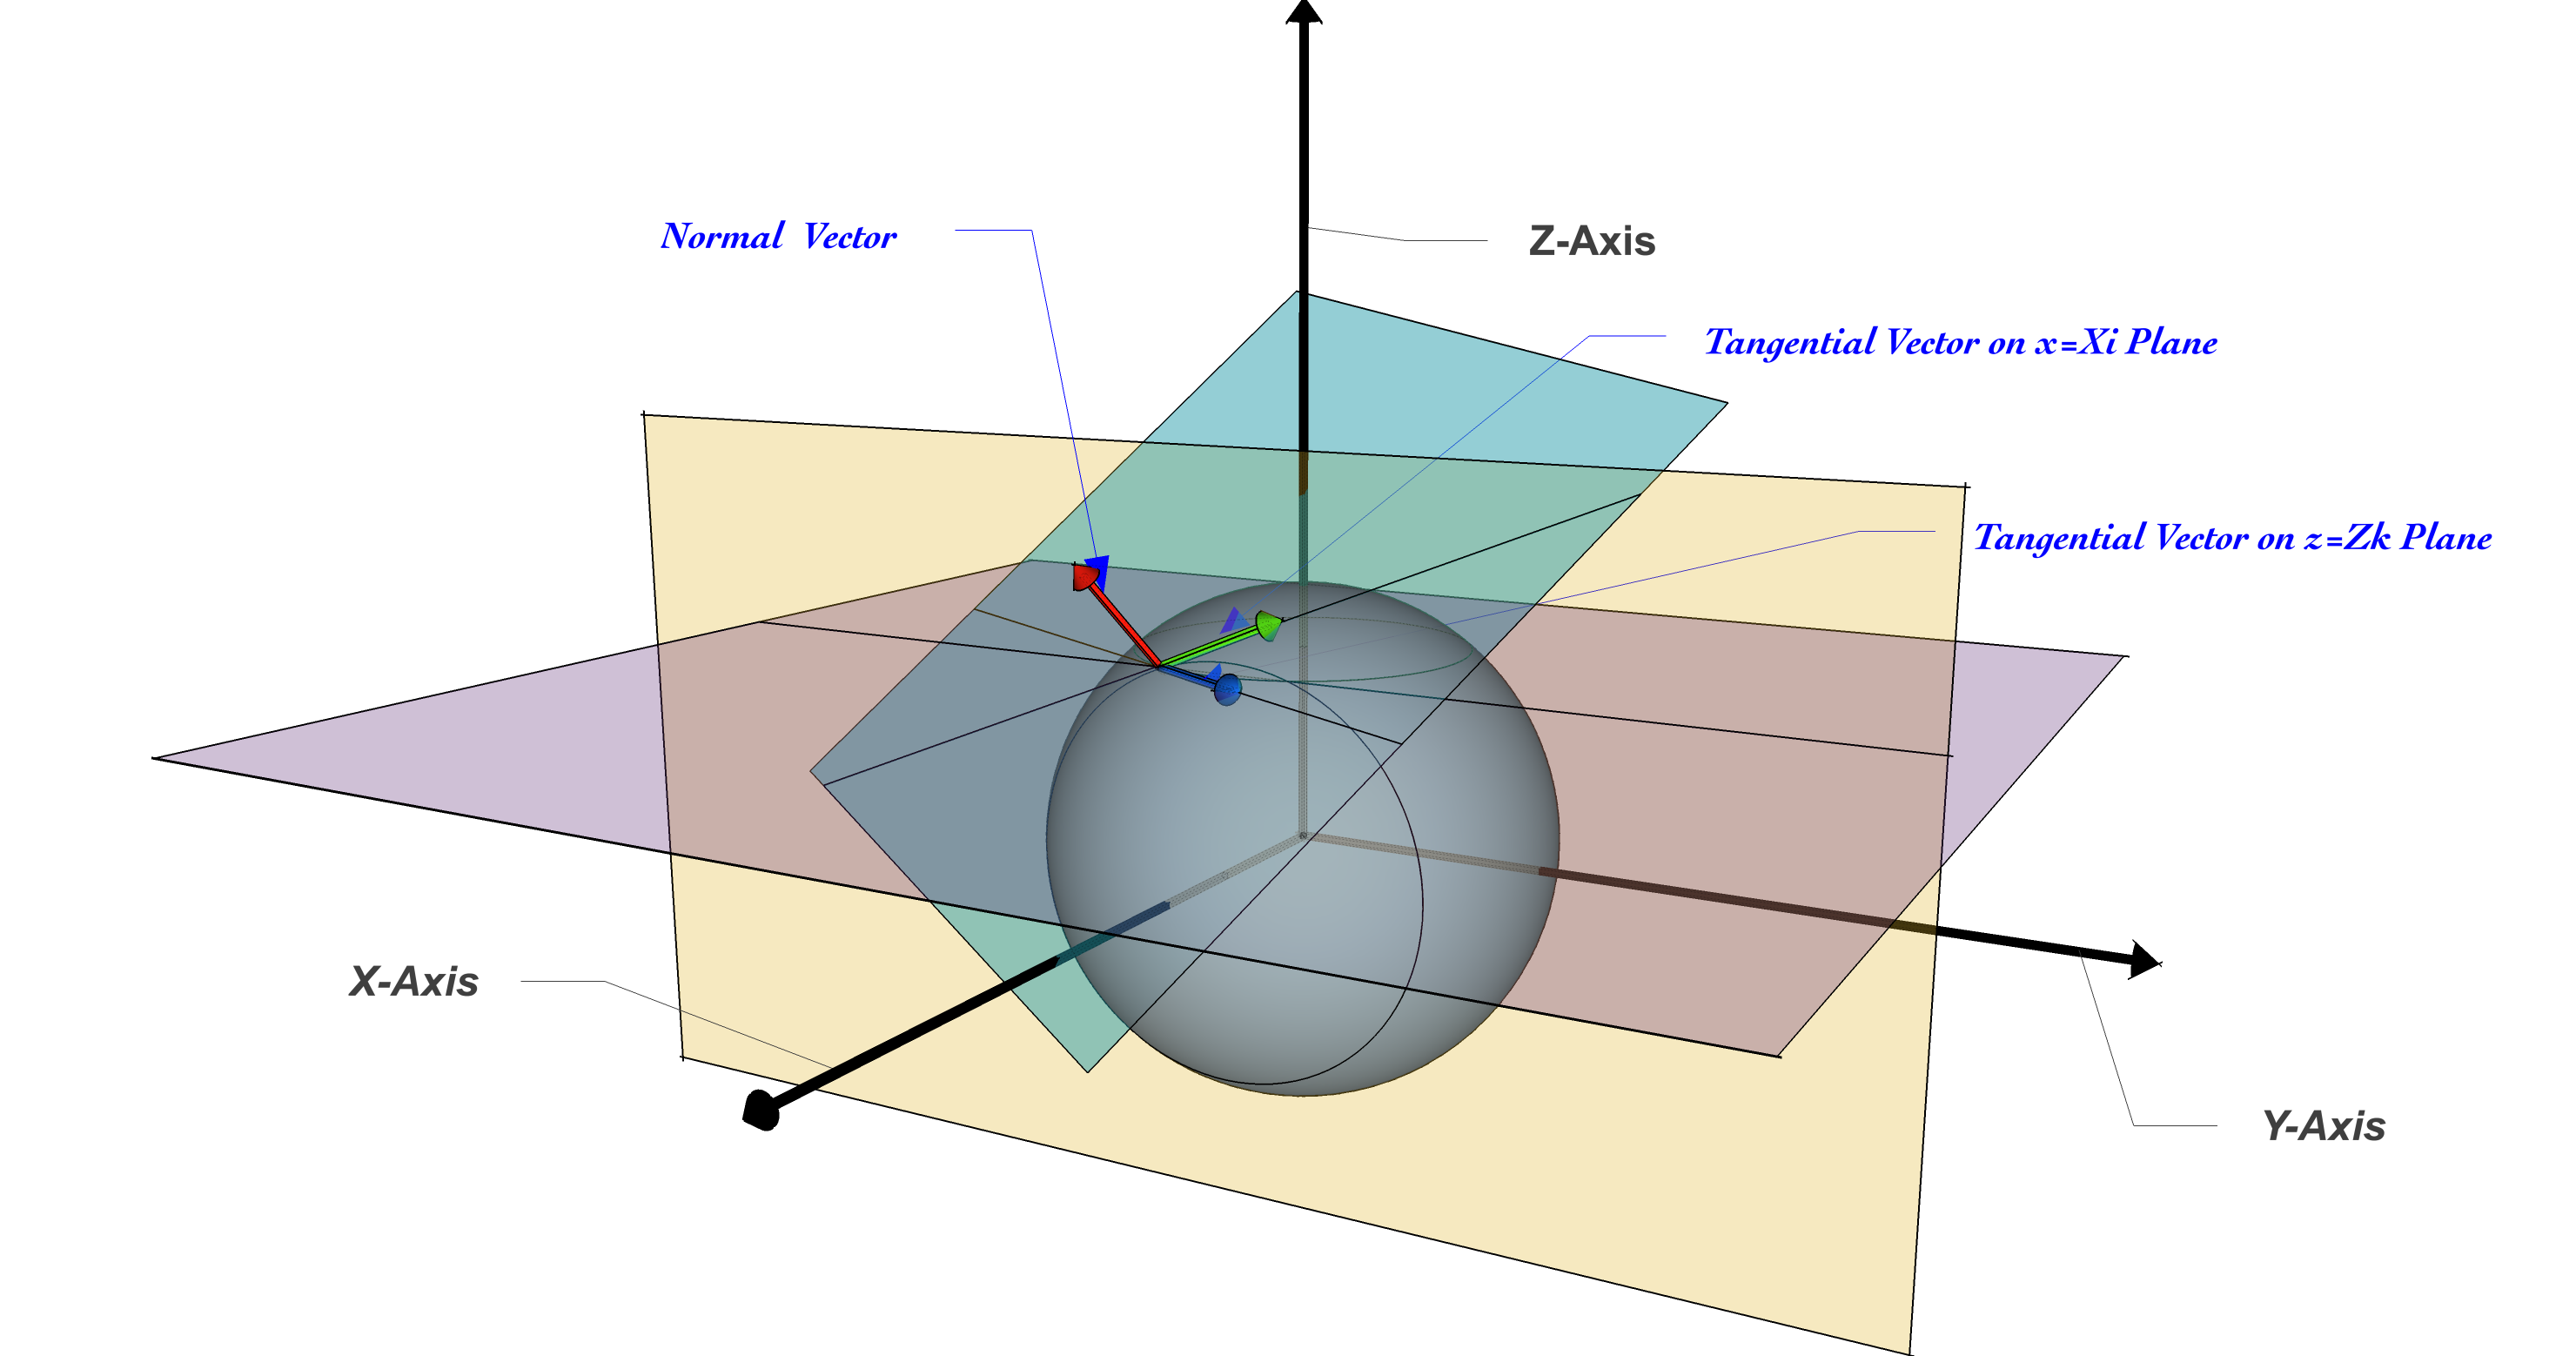
\includegraphics[width=17cm]{../figures/Local-Coordinate.png}
	\end{center}
	\caption{Non-orthogonal tangential directions $\eta$ and $\zeta$. Here at an interface point with
		the normal direction $\xi$ (red), $\eta$ and $\zeta$ are determined by intersecting the tangential plane (turquoise) with the place $x=x_i$ (yellow) and $z=z_k$ (mauve), respectively. 	
	}
	\label{fig:local_coordinate}
\end{figure*}
%
The local coordinate system $(\xi,\eta,\zeta)$ at the interface point IPY
can be related to the global $xyz$ coordinate system by a transformation matrix $P$
%
\begin{equation}\label{orginal-to-local}
\begin{bmatrix}
\xi \\
\eta \\
\zeta 
\end{bmatrix}
=
P
\begin{bmatrix}
x \\
y \\
z
\end{bmatrix}.
\end{equation}
%
In the $y-$direction, the transformation matrix $P_y$ is provided by
%
\begin{equation}\label{P in y-direction}
P_y=
\begin{bmatrix}
n_{x} &                 n_{y}                    &      n_{z}       \\
0     & \frac{n_{z}}{\sqrt{n^{2}_{y}+n^{2}_{z}}} & -\frac{n_{y}}{\sqrt{n^{2}_{y}+n^{2}_{z}}} \\
\frac{n_{y}}{\sqrt{n^{2}_{x}+n^{2}_{y}}} & -\frac{n_{x}}{\sqrt{n^{2}_{x}+n^{2}_{y}}} & 0
\end{bmatrix}.
\end{equation}
%
Similarly, one can construct the transformation matrix $P_x$ in the $x-$direction
%
\begin{equation}\label{P in x-direction}
P_x=
\begin{bmatrix}
n_{x}                                    &   n_{y}       &      n_{z}       \\
\frac{n_{z}}{\sqrt{n^{2}_{x}+n^{2}_{z}}} & 0             & -\frac{n_{x}}{\sqrt{n^{2}_{x}+n^{2}_{z}}} \\
\frac{n_{y}}{\sqrt{n^{2}_{x}+n^{2}_{y}}} & -\frac{n_{x}}{\sqrt{n^{2}_{x}+n^{2}_{y}}} & 0
\end{bmatrix},
\end{equation}
%
and $P_z$ in the $z-$direction
%
\begin{equation}\label{P in z-direction}
P_z =
\begin{bmatrix}
n_{x} &                   n_{y}                  &                     n_{z}                \\
0     & \frac{n_{z}}{\sqrt{n^{2}_{y}+n^{2}_{z}}} & -\frac{n_{y}}{\sqrt{n^{2}_{y}+n^{2}_{z}}} \\
\frac{n_{z}}{\sqrt{n^{2}_{x}+n^{2}_{z}}}         & 0 &  -\frac{n_{x}}{\sqrt{n^{2}_{x}+n^{2}_{z}}}
\end{bmatrix},
\end{equation}
%
respectively, for interface point $(x_{\Gamma},y_{j},z_{k})$ and $(x_{i},y_{j},z_{\Gamma})$.

\subsection{Tensor product decomposition of jump conditions}
After the local $\xi \eta \zeta -$coordinate system at the interface point IPY is obtained, one can differentiate the zeroth order jump condition $[u]=\phi$ in \eqref{interface_jumps} along the two tangential directions ($\eta$ and $\zeta$) to obtain two additional jump conditions 
\begin{equation}\label{jump_tan}
[u_{\eta}] = \phi_{\eta}, \quad \mbox{and} \quad [u_{\zeta}] = \phi_{\zeta}.
\end{equation}
Note that the known jump conditions \eqref{interface_jumps} and \eqref{jump_tan} 
are in normal and tangential directions, and can not be applied in a 1D manner
in the ADI algorithm, because they are not along the $x-$, $y-$ or $z-$axis. 

The desired Cartesian jump conditions, i.e., $[\alpha u_{x}]$, $[\alpha u_{y}]$ and $[\alpha u_{z}]$, can be obtained through coordinate transformation, 
%
\begin{equation} \label{local-to-orginal}
\begin{pmatrix}
\psi_{x}    \\
\psi_{y}    \\
\psi_{z}
\end{pmatrix}
:=
\begin{pmatrix}
[\alpha u_{x}]   \\
[\alpha u_{y}]   \\
[\alpha u_{z}]
\end{pmatrix}
=
P^{-1}
\begin{pmatrix}
[\alpha u_{\xi}]    \\
[\alpha u_{\eta}]   \\
[\alpha u_{\zeta}]
\end{pmatrix},
\end{equation}
%
where $[\alpha u_{\xi}] = \psi$ is known in (\ref{interface_jumps}), while  $[\alpha u_{\eta}]$ and $[\alpha u_{\zeta}]$ are unknown. 
Notice that the transformation matrix $P$ is singular only when the tangential plane is parallel to one of $xy-$, $xz-$, or $yz-$ plane. In such a case, the flux jump condition $[\alpha u_{\xi}] = \psi$ is simply the desired 1D jump condition in $z$, $y$ or $x$ direction. Besides this degenerate case, $P^{-1}$ in \eqref{local-to-orginal} always exists and can be calculated either analytically or numerically.

The unknown jumps of $[\alpha u_{\eta}]$ and $[\alpha u_{\zeta}]$ can be calculated with the aid of \eqref{jump_tan}
\begin{align}
[\alpha u_{\eta}] = \alpha^{+}\phi_{\eta} + (\alpha^{+}-\alpha^{-})u^{-}_{\eta} ~~~ \mbox{or} ~~~ [\alpha u_{\eta}]  = \alpha^{-}\phi_{\eta} + (\alpha^{+}-\alpha^{-}) u^{+}_{\eta}, \label{alpha u_eta}    \\
[\alpha u_{\zeta}] = \alpha^{+}\phi_{\zeta} + (\alpha^{+}-\alpha^{-}) u^{-}_{\zeta} ~~~ \mbox{or} ~~~ [\alpha u_{\zeta}] = \alpha^{-}\phi_{\zeta} + (\alpha^{+}-\alpha^{-}) u^{+}_{\zeta}. \label{alpha u_zeta}
\end{align}
Computationally, we will approximate two tangential derivatives $u_{\eta}$ and $u_{\zeta}$, in either $+$ or $-$ side, for determining $[\alpha u_{\eta}]$ and $[\alpha u_{\zeta}]$ numerically. 
Once $[\alpha u_{\eta}]$ and $[\alpha u_{\zeta}]$ are obtained, they are coupled with  $[\alpha u_{\xi}] = \psi$ to deliver 1D jump conditions in Cartesian directions: 
$ [\alpha u_x]=\psi_x$, $ [\alpha u_y]=\psi_y$, and $ [\alpha u_z]=\psi_z$. 
Thus, the key in the tensor product decomposition of 3D jump conditions is how to approximate two tangential derivatives accurately. 

\subsection{Tangential derivative approximations}
A new algorithm is proposed in this paper to approximate tangential derivatives, which is novel in two folds. 
First, since each of the non-orthogonal tangential directions is contained in a 2D Cartesian grid plane, the tangential derivatives can be computed in a 2D manner. If the orthogonal tangential directions are adopted as in the classical MIB 3D scheme \cite{yu2007three}, one tangential derivative has to be calculated as a 3D problem. Obviously, the present algorithm is  simpler. 
Second, both positive and negative side information will be employed for calculating tangential derivatives, while in our previous 2D matched ADI methods  \cite{zhao2015matched,li2017matched}, the tangential derivatives are calculated only from the positive side. 
In 3D, the interface $\Gamma$ becomes geometrically more complicated, so that a more robust algorithm has to be developed in this work. 


We illustrate the proposed algorithm by considering $u_{\zeta}$ at the interface point $(x_i,y_{\Gamma},z_k)$, and $u_{\eta}$ can be treated similarly. Since the $\zeta$ direction is contained in a plane $z=z_{k}$, all involved points are in this plane. Thus, the numerical scheme  can be shown in a $x$-$y$ coordinate, see Fig. \ref{fig:tangential_approximation}(a).
Here  we assume $y_{j-1} \le y_{\Gamma} \le y_{j}$ and denote the interface point (and other points) simply as $(x_i,y_{\Gamma})$ by dropping $z=z_k$. 
If $\Gamma$ is locally convex with respect to $\Omega^-$, the approximation of $u^{+}_{\zeta}$ by nearby on-grid values from the outer domain $\Omega^+$ produces a better precision, while for a local concave curve, it is better to approximate $u^{-}_{\zeta}$ from  $\Omega^-$. For a situation shown in Fig. \ref{fig:tangential_approximation}(a) where the interface $\Gamma$ has an inflection, an optimization procedure is designed to select a better approximation from either $+$ or $-$ side. In fact, we apply the same optimization procedure for all interface points so that one can automatically select $u^{+}_{\zeta}$ or $u^{-}_{\zeta}$ based on the local geometry. 

In our algorithm, the auxiliary and supporting nodes for approximating $u^{+}_{\zeta}$ and $u^{-}_{\zeta}$ are first determined. As shown in Fig. \ref{fig:tangential_approximation}(a), the interface point $(x_i,y_{\Gamma})$ is marked with a purple square. Two auxiliary points$(x_{i-1},y_{\Gamma-1})$ and $(x_{i+1},y_{\Gamma+1})$ (purple rectangles in Figure \ref{fig:tangential_approximation}(a)) along the $\zeta$ line are chosen to form a central difference approximation for the $u_{\zeta}$
\begin{equation}\label{D_zeta}
u^{\pm}_{\zeta} (x_i,y_{\Gamma})\approx \frac{u^{\pm}(x_{i+1},y_{\Gamma+1}) - u^{\pm}(x_{i-1},y_{\Gamma-1})}{2 \Delta \zeta}, 
\end{equation}
where $\Delta \zeta$ is the distance between $(x_i,y_{\Gamma})$ and $(x_{i-1},y_{\Gamma-1})$. The auxiliary values will be interpolated/extrapolated by using supporting nodal values from the same side. 
Referring to Figure \ref{fig:tangential_approximation}(a), $u^{+}(x_{i+1},y_{\Gamma+1})$ and $u^{+}(x_{i-1},y_{\Gamma-1})$ will be extrapolated by six supporting nodes below $\Gamma$ (blue circles), while $u^{-}(x_{i+1},y_{\Gamma+1})$ and $u^{-}(x_{i-1},y_{\Gamma-1})$ are approximated by six  supporting nodes above $\Gamma$ (orange circles). The selection of $u^{+}_{\zeta}$ or $u^{-}_{\zeta}$ is according to the total distance between supporting nodes and auxiliary nodes. For Fig. \ref{fig:tangential_approximation}(a), we define
\begin{align}
d^+ & =\sum_{J=2}^4 |y_{\Gamma+1}-y_{j-J}| 
+\sum_{J=0}^2 |y_{\Gamma-1}-y_{j-J}|,   \\
d^- & =\sum_{J=-1}^1 |y_{\Gamma+1}-y_{j+J}| 
+\sum_{J=1}^3 |y_{\Gamma-1}-y_{j+J}|. 
\end{align}    
If $d^+ > d^-$, we calculate $u^{-}_{\zeta}$ by using \eqref{D_zeta} from the negative side. Otherwise, we approximate $u^{+}_{\zeta}$ by using \eqref{D_zeta} from the positive side. Then the auxiliary values are extrapolated by six supporting values. 


%
\begin{figure*}[!ht]
	\begin{center}
		\resizebox{\textwidth}{!}{
			\begin{tabular}{ccc}
				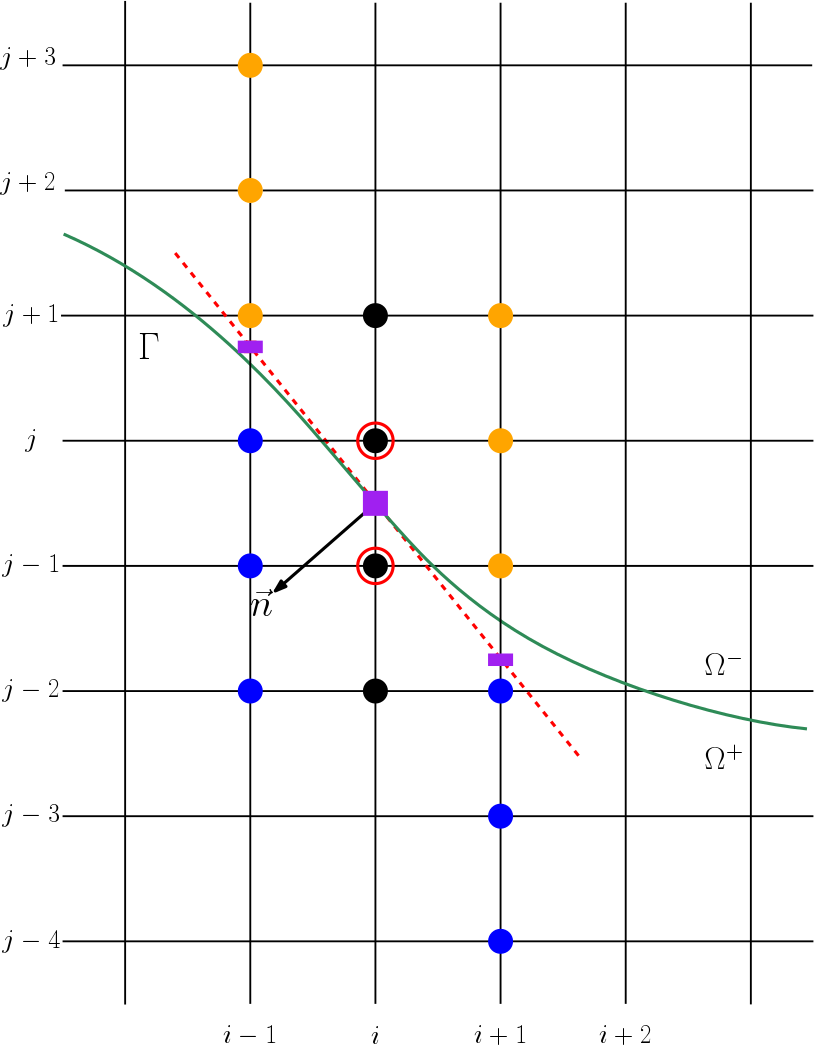
\includegraphics[width=7cm]{../figures/Tangential-Approximation.png} & \quad & 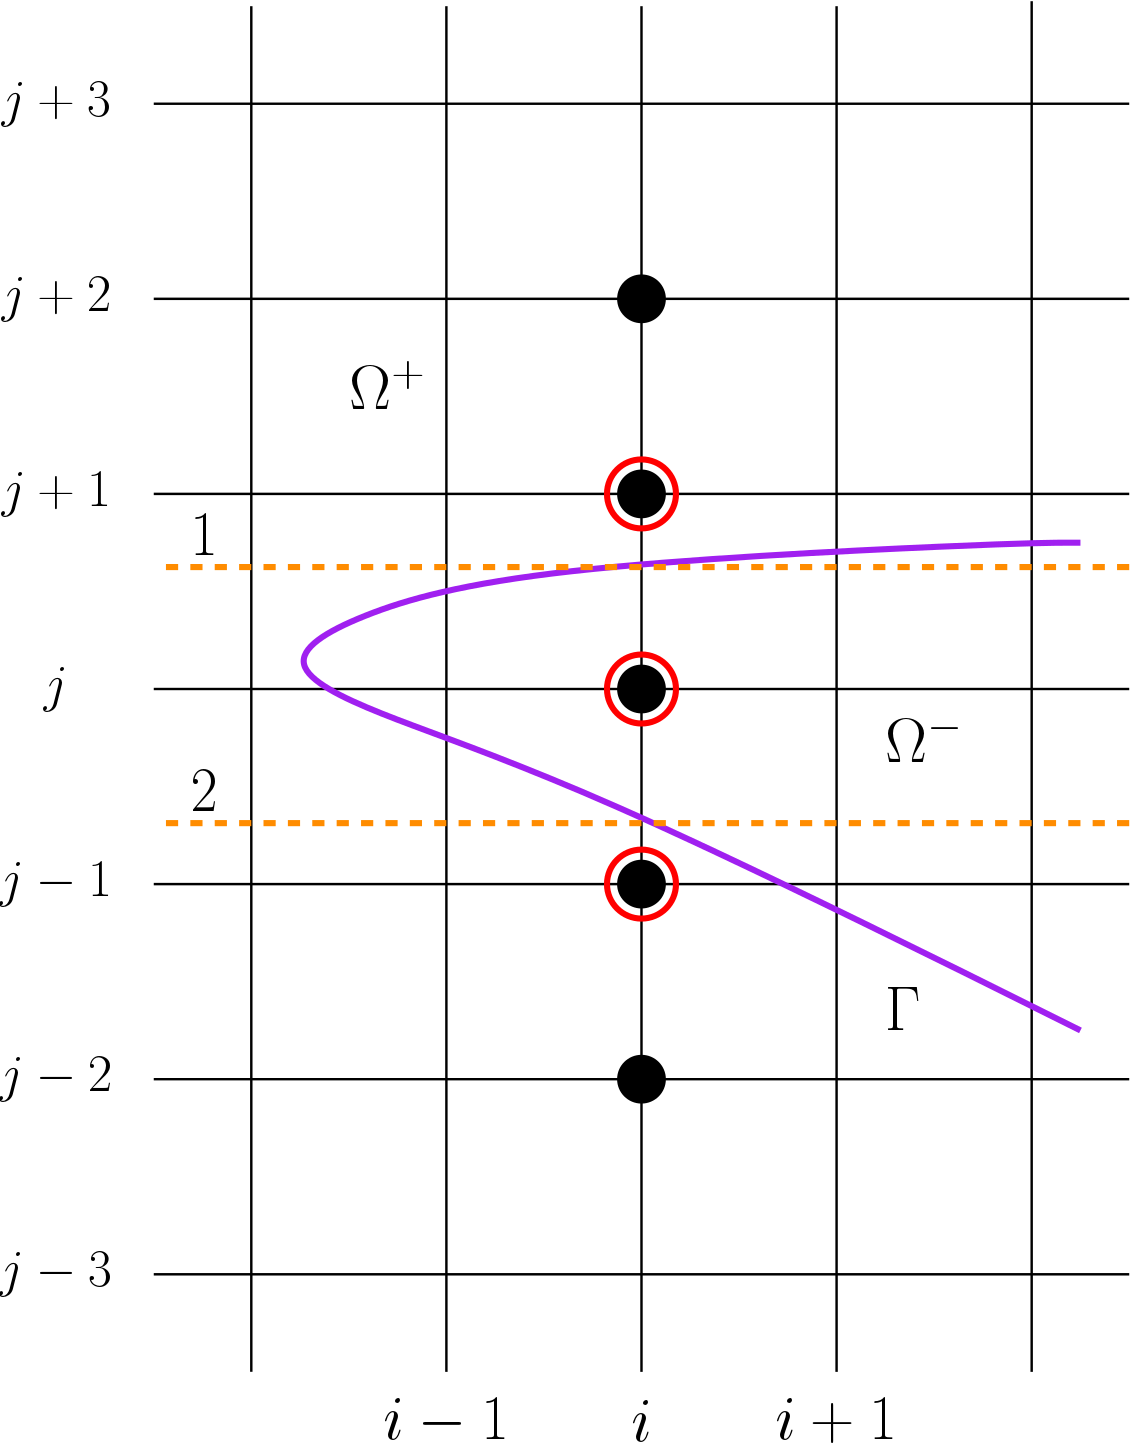
\includegraphics[width=7cm]{../figures/Corner.png} \\ 
				\ \textbf{(a)} & \quad & \textbf{(b)}
		\end{tabular}}
	\end{center}
	\caption{Tangential derivative approximation and MIB interface treatment. 
		(a). The tangential derivative at the interface point (purple square) is approximated through two auxiliary points (purple rectangles). Each auxiliary value will be extrapolated by three supporting nodes from the same side (positive or negative). An optimization procedure is designed to automatically select either positive or negative side for approximating tangential derivatives. The MIB 1D jump condition enforcement is also illustrated, which involves four nodes (black filled circles) and two fictitious nodes (red open circles). 
		(b). In a corner MIB treatment of 1D jump conditions,  five nodes (black filled circles) and three fictitious nodes (red open circles) are involved. Here two interface points $(x_i,y_{\Gamma1},z_k)$ and $(x_i,y_{\Gamma2},z_k)$ are the intersection points of $\Gamma$ with two dashed lines. }
	\label{fig:tangential_approximation}
\end{figure*}
%

The time interference is a subtle issue in this process. 
Note that at this stage of approximation, function values at the future time $t=t_{m+1}$ are unknown. 
So, we can only use the known function values at the current time step $t=t_{m}$ for 
the six supporting nodes. 
Consequently, the calculated tangential derivatives are held at $t_{m}$, and 
we denote them as $(u^{-}_{\zeta})^m$ and $(u^{+}_{\zeta})^m$. 
However, the finite difference correction \eqref{delta_yy} is intended to be conducted at $t_{m+1}$. Hence, in \eqref{local-to-orginal}, \eqref{alpha u_eta}, and \eqref{alpha u_zeta},  we specify analytically known jumps at $t_{m+1}$, i.e., $\psi^{m+1}$, $\phi_{\eta}^{m+1}$, and  $\phi_{\zeta}^{m+1}$, for a better accuracy. 
Mathematically, the calculated jumps $\psi_x$, $\psi_y$, and $\psi_z$ can be expressed as a linear combination of some supporting nodal values at $t_m$, and $\psi^{m+1}$, $\phi_{\eta}^{m+1}$, and  $\phi_{\zeta}^{m+1}$ at $t_{m+1}$. 
With hybrid contributions from two time levels, the Cartesian jump values $\psi_x$, $\psi_y$, and $\phi_z$ mainly depend on the supporting function values at $t_m$.
Thus, we will denote them as $\psi^m_x$, $\psi^m_y$, and $\psi^m_z$.
This finishes the first stage of the spatial discretization of the matched ADI method. 

\subsection{1D jump conditions enforcement}
In the second stage of the matched ADI method, we impose the decomposed 1D jump conditions
\begin{equation}\label{jump1D}
[u]=\phi^{m+1}, \quad [\alpha u_x]=\psi_x^m, \quad [\alpha u_y]=\psi_y^m, \quad [\alpha u_z]=\psi_z^m, 
\end{equation}
to correct the finite difference operators $\delta_{xx}$, $\delta_{yy}$ and $\delta_{zz}$ in \eqref{delta_yy} by using the MIB scheme
\cite{zhao2004high,zhou2006high,yu2007three,yu2007matched}.
We will also only consider $\delta_{yy}$ here for simplicity. 
For two irregular points, $\delta_{yy}$ at time step $t_{m+1}$ is modified to be 
%
\begin{eqnarray} \label{MIB_delta_yy}
\delta_{yy} u^{m+1}_{i,j,k} &:=& \frac{1}{\Delta y^{2}} (\tilde{u}^{m+1}_{i,j-1,k} - 2 u^{m+1}_{i,j,k} + u^{m+1}_{i,j+1,k}), \quad \mbox{in}~ \Omega^- \nonumber \\
\delta_{yy} u^{m+1}_{i,j-1,k} &:=& \frac{1}{\Delta y^{2}} (u^{m+1}_{i,j-2,k} - 2 u^{m+1}_{i,j-1,k} + \tilde{u}^{m+1}_{i,j,k}), \quad \mbox{in}~ \Omega^+
\end{eqnarray}
%
where $\tilde{u}^{m+1}_{i,j-1,k}$ and $\tilde{u}^{m+1}_{i,j,k}$ are two fictitious value at node $(x_{i},y_{j-1},z_{k})$ and $(x_{i},y_{j},z_{k})$, respectively, as shown in Fig. \ref{fig:tangential_approximation}(a). These two fictitious values $\tilde{u}^{m+1}_{i,j-1,k}$ and $\tilde{u}^{m+1}_{i,j,k}$ are determined by discretizing two jump conditions in \eqref{jump1D}. 
%
\begin{align}
\omega^{+}_{0,1}u^{m+1}_{i,j-2,k}+\omega^{+}_{0,2}u^{m+1}_{i,j-1,k}+\omega^{+}_{0,3}\tilde{u}^{m+1}_{i,j,k}&=\omega^{-}_{0,1}\tilde{u}^{m+1}_{i,j-1,k}+\omega^{-}_{0,2}u^{m+1}_{i,j,k}+\omega^{-}_{0,3}u^{m+1}_{i,j+1,k}+\phi^{m+1}, \label{irregular_jump_1}\\
\alpha^{+}(\omega^{+}_{1,1}u^{m+1}_{i,j-2,k}+\omega^{+}_{1,2}u^{m+1}_{i,j-1,k}+\omega^{+}_{1,3}\tilde{u}^{m+1}_{i,j,k})&=\alpha^{-}(\omega^{-}_{1,1}\tilde{u}^{m+1}_{i,j-1,k}+\omega^{-}_{1,2}u^{m+1}_{i,j,k}+\omega^{-}_{1,3}u^{m+1}_{i,j+1,k})+\psi_{y}^{m}, \label{irregular_jump_2}
\end{align}
%
where $\omega^{+}_{i,j}$ and $\omega^{-}_{i,j}$ are finite different weights \cite{fornberg1998classroom} for interface surrounding nodes from outer domain $\Omega^{+}$ or inner domain $\Omega^{-}$. The subscript $i$ represents the interpolation when $i=0$ and first order approximation when $i=1$, and the subscript $j$ represents the indicies of related grid nodes. Solving \eqref{irregular_jump_1} and \eqref{irregular_jump_2} allows 
$\tilde{u}^{m+1}_{i,j-1,k}$ and $\tilde{u}^{m+1}_{i,j,k}$ 
to be written as linear combinations of $u^{m+1}_{i,j-2,k}$, $u^{m+1}_{i,j-1,k}$, $u^{m+1}_{i,j,k}$, $u^{m+1}_{i,j+1,k}$, and two jump values $\phi^{m+1}$ and $\psi_{y}^m$.
By  substituting $\tilde{u}^{m+1}_{i,j-1,k}$ and $\tilde{u}^{m+1}_{i,j,k}$  into \eqref{MIB_delta_yy}, $\delta_{yy} u^{m+1}_{i,j,k}$ and $\delta_{yy} u^{m+1}_{i,j-1,k}$ are represented by four surrounding on-grid values at $t_{m+1}$, i.e., $u^{m+1}_{i,j-2,k}$, $u^{m+1}_{i,j-1,k}$, $u^{m+1}_{i,j,k}$, $u^{m+1}_{i,j+1,k}$, four jump values at $t_{m+1}$, i.e., $\phi^{m+1}$, $\psi^{m+1}$, $\phi_{\eta}^{m+1}$, and  $\phi_{\zeta}^{m+1}$, 
six values at nodes on plane $z=z_{k}$ at $t_{m}$,
and six values at nodes on plane $x=x_{i}$ at $t_{m}$.

It is possible that the interface $\Gamma$ changes rapidly and cuts one grid line twice within a short distance.
If there are at least two grid nodes in between these two intersection points, the above mentioned 
approximation can be conducted. 
When there is only one node (it is called a corner point), a MIB corner treatment has to be adopted. 
For instance, in Fig. \ref{fig:tangential_approximation}(b),
a corner treatment is needed for $(x_{i-1},y_j,z_k)$ and $(x_{i},y_j,z_k)$ along $y$ direction, 
while the usual MIB scheme can be used for other irregular points in $\Omega^-$. 
Since the present jump condition enforcement is of 1D nature, 
the corner treatment developed in our previous 2D matched ADI method \cite{zhao2015matched} can be simply utilized for 3D problems. 
Essentially, we need to enforce jump conditions at two interface points simultaneously. 
We omit the details but briefly describe the idea here by considering $(x_{i},y_j,z_k)$
in Fig. \ref{fig:tangential_approximation}(b). 
At this corner point, three fictitious values, $\tilde{u}^{m+1}_{i,j-1,k}$, $\tilde{u}^{m+1}_{i,j,k}$ and $\tilde{u}^{m+1}_{i,j+1,k}$, are calculated together with one additional fictitious value, either $\tilde{u}^{m+1}_{i,j-2,k}$ or $\tilde{u}^{m+1}_{i,j+2,k}$ depending on which node is closer, in order to maintain the convergence rate. The four fictitious values are solved by a system of four equations, built from imposing the jump conditions at the interface points on both sides of the corner point, following similar formulation as in (\ref{irregular_jump_1})-(\ref{irregular_jump_2}). 
By  substituting fictitious values into \eqref{MIB_delta_yy}, $\delta_{yy} u^{m+1}_{i,j,k}$ is  represented by five surrounding on-grid values at $t_{m+1}$, i.e., ${u}^{m+1}_{i,j-2,k}$, ${u}^{m+1}_{i,j-1,k}$, ${u}^{m+1}_{i,j,k}$, ${u}^{m+1}_{i,j+1,k}$ and ${u}^{m+1}_{i,j+2,k}$, 
eight jump values at $t_{m+1}$, i.e., $\phi^{m+1}$, $\psi^{m+1}$, $\phi_{\eta}^{m+1}$, and  $\phi_{\zeta}^{m+1}$ at two interface points $(x_i,y_{\Gamma1},z_k)$ and $(x_i,y_{\Gamma2},z_k)$, and a total of 24 supporting nodal values at $t_m$. 
This finishes the second stage of the spatial discretization of the matched ADI method. In this entire process, a spatially second order of accuracy is guaranteed throughout the domain. 

Symbolically, the aforementioned MIB corrections of the finite difference operators $\delta_{xx}$, $\delta_{yy}$, and $\delta_{zz}$ can be expressed as \cite{zhao2015matched,li2017matched}
%
\begin{eqnarray} 
\delta_{xx} u^{m+1}_{i,j,k} &=& D_{xx} u^{m+1}_{i,j,k} + B_{x} u^{m}_{i,j,k} + \Phi_{x}^{m+1}, \label{delta_xx_operator} \\ 
\delta_{yy} u^{m+1}_{i,j,k} &=& D_{yy} u^{m+1}_{i,j,k} + B_{y} u^{m}_{i,j,k} + \Phi_{y}^{m+1}, \label{delta_yy_operator} \\
\delta_{zz} u^{m+1}_{i,j,k} &=& D_{zz} u^{m+1}_{i,j,k} + B_{z} u^{m}_{i,j,k} + \Phi_{z}^{m+1}, \label{delta_zz_operator}
\end{eqnarray}
%
where $D_{xx}$, $D_{yy}$, and $D_{zz}$ are perturbed operators which have a band-width 4 for a usual irregular node, and a band-width 5 for a corner node. The operators $B_{x}$, $B_{y}$, and $B_{z}$ are due to tangential derivative approximations, which have a band-width 12 for a usual irregular node, and a band-width 24 for a corner node. The jump terms $\Phi^{m+1}_{x}$, $\Phi^{m+1}_{y}$, and $\Phi^{m+1}_{z}$ are the sums of 4 and 8 jump values, respectively, for a usual irregular node and corner node.

%%%%%%%%%%%%%%%%%%%%%%%%%%%%%
\section{A new ADI method with less perturbation terms}
Because the MIB corrected finite difference operators in \eqref{delta_xx_operator}  - 
\eqref{delta_zz_operator} involves two time levels $t_m$ and $t_{m+1}$, a direct application of them to approximate derivatives in the standard ADI scheme \eqref{D_ADI} is questionable. In particular, the intermediate functions $u^*$ and $u^{**}$ are at unknown fractional time instants between  $t_m$ and $t_{m+1}$, so that one does not know how to specify a time for them. One possible choice here is to use $t_{m+1}$ for approximating derivatives of $u^*$ and $u^{**}$ in \eqref{D_ADI}, while derivatives of $u^m$ on the right hand sides of \eqref{D_ADI} are evaluated at $t_m$. As a consequence, when one eliminates the intermediate functions $u^*$ and $u^{**}$, similar to (\ref{connection_1}) and (\ref{connection_2}) in the semi-discretized form, the difference between such an ADI scheme and the implicit Euler scheme involves many perturbation terms. 

To overcome the aforementioned difficulty, 
we propose a new ADI method which minimizes the number perturbation terms when comparing it with the implicit Euler scheme. Our idea is to apply the finite difference operators \eqref{delta_xx_operator}  - \eqref{delta_zz_operator} to the implicit Euler scheme \eqref{implicit_Euler}, which then can be rewritten as
\begin{equation} \label{implicit_Euler2}
\frac{u^{m+1}_{i,j,k}-u^{m}_{i,j,k}}{\alpha \Delta t} = 
D_{xx} u^{m+1}_{i,j,k} +D_{yy} u^{m+1}_{i,j,k} +D_{zz} u^{m+1}_{i,j,k} + F^{m+1}_{i,j,k},
\end{equation}
where $F^{m+1}_{i,j,k}=(B_{x}+B_{y}+B_{z})u^{m}_{i,j,k}+\Phi^{m+1}_{x}+\Phi^{m+1}_{y}+\Phi^{m+1}_{z}+\frac{1}{\alpha}f^{m+1}_{i,j,k}$. 
The Douglas-Rachford ADI method for the implicit Euler scheme \eqref{implicit_Euler2} is simply given as 
\begin{align}
(\frac{1}{\alpha}-\Delta t D_{xx}) u^{*}_{i,j,k}   &= (\frac{1}{\alpha} + \Delta t(D_{yy} + D_{zz})) u^{m}_{i,j,k} + \Delta t F^{m+1}_{i,j,k}, \nonumber \\
(\frac{1}{\alpha}-\Delta t D_{yy}) u^{**}_{i,j,k}  &= \frac{1}{\alpha} u^{*}_{i,j,k} - \Delta t D_{yy} u^{m}_{i,j,k}, \label{D_ADI_operator}  \\
(\frac{1}{\alpha}-\Delta t D_{zz}) u^{m+1}_{i,j,k} &= \frac{1}{\alpha} u^{**}_{i,j,k} - \Delta t D_{zz} u^{m}_{i,j,k}. \nonumber 
\end{align}
%
Similarly, we can show the difference between such an ADI and the implicit Euler schemes is 
\begin{equation} \label{perturbation}
- \alpha^2 \Delta t^{2} (D_{xx}D_{yy} + D_{xx}D_{zz} + D_{yy}D_{zz} ) (u^{m+1}_{i,j,k}-u^{m}_{i,j,k} )
+ \alpha^3 \Delta t^{3} D_{xx}D_{yy} D_{zz}  (u^{m+1}_{i,j,k}-u^{m}_{i,j,k} ),
\end{equation}
which is in consistent with the semi-discretized form. The temporal order of the proposed ADI scheme is obviously one, i.e., $O(\Delta t)$. 

In our computations, the boundary conditions for $u^*$ and $u^{**}$ in \eqref{D_ADI_operator} are assumed to be the same as $u^{m+1}$, i.e., at time step $t=t_{m+1}$. 
We note that the matrix coefficients of $D_{xx}$, $D_{yy}$,  $D_{zz}$, $B_{x}$, $B_{y}$, and $B_{z}$ 
only require to be calculated once before the time evolution, because these spatial discretization coefficients
only depend on interface geometry and grid nodes, which are time invariant. 
Then, these sparse coefficients and their column and row indexes are stored and reused in each time step,
without too much computational overhead. 
Algebraically, the corrected operators $D_{xx}$, $D_{yy}$, and $D_{zz}$ are perturbed tridiagonal matrices
with only a few rows having a band-width four (usual irregular node) or five (corner node). 
A fast algorithm has been developed in \cite{zhao2015matched} to invert such matrices efficiently at each time step,
in which 
these systems are first converted to tridiagonal ones by row-eliminations and solved by the Thomas algorithm \cite{strikwerda2004}. 
Taking the advantage of the Thomas algorithm, the proposed 3D matched ADI method has a computational cost of order $O(N)$ for each time step, where $N$ is the total spatial degree of freedom.



Neglecting the perturbation terms (\ref{perturbation}), the stability of the ADI scheme \eqref{D_ADI_operator} is essentially governed by that of the implicit Euler scheme \eqref{implicit_Euler2}. Denote ${\bf U}^m$ as a vector of dimension $N$ containing all $u$ values at the time $t_m$. One can rewrite  the implicit Euler scheme \eqref{implicit_Euler2} into the matrix form
\begin{equation}
{\bf D} {\bf U}^{m+1} = {\bf B} {\bf U}^m + {\bf C},
\end{equation}
where ${\bf D}$ and ${\bf B}$ are matrices of dimension $N \times N$, and ${\bf C}$ is a vector of dimension $N$. 
Note that ${\bf B}$ is due to the approximation of tangential
derivatives by some function values of $u$ at time $t_m$. The sparse elements of ${\bf B}$ are distributed
in a rather random fashion - their locations depend on the interface geometry and grid size. 
Generally speaking, a von Neumann type stability analysis is infeasible. 
Alternatively, the stability analysis of the proposed ADI scheme can be conducted as in \cite{zhao2015matched},
through numerically verifying whether the spectral radius of the magnifying matrix ${\bf D}^{-1} {\bf B}$ is not greater than one. 
However, since $N$ is a very large number for 3D problems, the eigenvalue computation is time consuming, and is thus skipped in the present study. 
Instead, the stability of the 3D matched ADI scheme is numerically examined in next section.  


%----------------------------------------------------------------------%
%                                                                      %
%                             Chapter 3                                %
%                                                                      %
%----------------------------------------------------------------------%
\chapter{\MakeUppercase{Comparison of different time splitting methods with variable diffusion coefficients}}

In the second part, unlike the governing equation in previous chapter, the diffusion coefficients $\alpha$ are now function of space. It's necessary to rewrite the governing equation, a typical parabolic interface problem involves a parabolic partial differential equation (PDE) for a function $u(\vec x)$ on both sides of the interface $\Gamma$.
%
\begin{equation}\label{heat_eqn_3}
\frac{\partial u(\vec{x})}{\partial t} = \nabla \cdot (\alpha(\vec{x}) \nabla u(\vec{x})) + f(\vec{x}), ~~~ \vec{x} \in \Omega\setminus\Gamma, ~~~ \Omega =\Omega^{-} \cup \Omega^{+}
\end{equation}
%
with appropriate imposed boundary conditions along the interface, 
%
\begin{equation}\label{interface_jumps_3}
\begin{split}    
[u](X) &:= u^{+} - u^{-} = \phi(X,t), \\
[\alpha u_{n}](X) &:= \alpha^{+}(X) \nabla u^{+} \cdot \vec {n}(X) - \alpha^{-}(X) \nabla u^{-} \cdot \vec {n}(X) = \psi(X,t), ~~~ \mbox{with} ~ X \in \Gamma
\end{split}
\end{equation}
%
where domain $\Omega$ is separated by interface $\Gamma$ into two sub-domains $\Omega^{-}$ and $\Omega^{+}$ and $\vec n(X)$ is the unit normal direction at a point $X$ on the interface pointing to $\Omega^{+}$ side. Meanwhile, we adopt $\vec x$ as a point to the domain without interface, while $X$ a point on the interface $\Gamma$. The following notations are chosen in this paper. The Cartesian coordinate system is taken into consideration with uniform meshes in a 3D finite rectangular domain $\Omega \subset \mathbb{R}^{3}$. Respectively, in $x$, $y$, and $z$ direction, the mesh sizes are chosen to be $\Delta x=h_{x}$, $\Delta y=h_{y}$ and $\Delta z=h_{z}$ with grid points $N_{x}$, $N_{y}$ and $N_{z}$. The time increment is denoted as $\Delta t$. The notation $u^{m}_{i,j,k} = u(x_{i},y_{j},z_{k},t_{m})$ denotes the value of numerical solution at the specific node $(x_{i}, y_{j}, z_{k})$ and a time step $t_{m}$. For all splitting methods, we are interested in updating all grid nodes from a time step $t_{m}$ to the next time step $t_{m+1} = t_{m} + \Delta t$.
%
%%%%%%%%%%%%%%%%%%%%%%%%%%%%%%%%%%%%%%%%%%%%%%%%%%%%%%%%%%%%%%%%%%%%%%%%%%%%%%%%%%
\section{Enforcing 3D jump conditions in 1D manner}
%
A well-known numerical method is called operator splitting which separates the original equation into several parts over a time step, computes the solution in each time step separately and then combines the solutions together to form a solution to the original equation. The two biggest advantages of operator splitting are stability and efficiency. It is much faster to compute solutions of the split terms than to compute the solution to the original problem directly. There exists many operator splitting method that can reduce a multidimensional problem into a set of independent one-dimensional problems. We will explore a few commonly used operator splitting methods in this paper and test their performances in the proposed parabolic interface problem with different variable diffusion coefficients. With central finite difference discretization in space, all the mentioned operator splitting methods will benefit from the tridiagonal structures, such that can be solved by Thomas algorithm not only accurately but efficiently as well.  
%
\subsection{Parabolic interface problem with variable coefficients}
%
One of the contribution in this section comparing with previous section is the capability of solving parabolic interface with variable diffusion coefficients in high dimensional space. In (\ref{interface_jumps_3}), the diffusion coefficients are no longer only a pair of piecewise constants along two sub-domains $\Omega^{-}$ and $\Omega^{+}$ but also denotes piecewise function with respect to the coordinates in three dimension along interface $\Gamma$. The governing equation (\ref{heat_eqn_3}) will be formed as
%
\begin{align} \label{discretized_eqn_3}
\frac{\partial u(x, y, z)}{\partial t} = 
&\frac{\partial}{\partial x}(\alpha(x,y,z) \frac{\partial u(x, y, z)}{\partial x}) + \\
&\frac{\partial}{\partial y}(\alpha(x,y,z) \frac{\partial u(x, y, z)}{\partial y}) + 
\frac{\partial}{\partial z}(\alpha(x,y,z) \frac{\partial u(x, y, z)}{\partial z}) + f(x, y, z), 
~ \mbox{in} ~ \Omega^{-} \cup \Omega^{+}, \nonumber
\end{align}
%
in three dimensional space, with diffusion coefficients as piecewise function $\alpha^{+}(x, y, z)$ in $\Omega^{+}$ and $\alpha^{-}(x, y, z)$ in $\Omega^{-}$.
%	
\subsection{Euler discretization with central finite difference}
We are favorable to implicit time evolution schemes to semi-discretirise (\ref{heat_eqn_3}) in time benefiting from the fact that, the equilibrium solution after long-term iteration are usually more meaningful and desirable. First, considering a simplified situation in which the exact solution is smooth throughout entire domain $\Omega$. Technically, there is no jump along interface $\Gamma$ due to the smoothness of analytical solution which yeilds a trivial jump conditions in (\ref{interface_jumps_3}). An classic implicit Euler discretization with standard central finite difference scheme is applied on (\ref{heat_eqn_3}) in a time interval $[t^{m}, t^{m+1}]$,
%
\begin{equation} \label{implicit_Euler_3}
\frac{u^{m+1}_{i,j,k}-u^{m}_{i,j,k}}{\Delta t} = 
\delta_{xx}^{\alpha} u^{m+1}_{i,j,k} + 
\delta_{yy}^{\alpha} u^{m+1}_{i,j,k} + 
\delta_{zz}^{\alpha} u^{m+1}_{i,j,k} + f^{m+1}, 
\end{equation}
%
where the superscript $m$ denotes the time step, and the subscript is utilized for spatial discretization at specific mesh node at $(x_i, y_j, z_k)$ in three dimensional space, not only the exact solution $u$ and source term $f$ but also the diffusion coefficient $\alpha$ are spatial dependent in all $x$, $y$ and $z$ directions. In (\ref{implicit_Euler_3}), Operators $\delta_{xx}^{\alpha}$, $\delta_{yy}^{\alpha}$ and $\delta_{zz}^{\alpha}$ are defined with caution to approximate the second partial derivatives $\frac{\partial}{\partial x}(\alpha \frac{\partial} {\partial x})$, $\frac{\partial}{\partial y}(\alpha \frac{\partial} {\partial y})$ and $\frac{\partial}{\partial z}(\alpha \frac{\partial} {\partial z})$ respectively, due to the spatial dependent diffusion coefficient $\alpha(x,y,z)$,
%
\begin{eqnarray} \label{delta_xx_3}
\delta_{xx}^{\alpha} u^{m+1}_{i,j,k} &:=  
\frac{1}{\Delta x^{2}} ~ (\alpha_{i-\frac{1}{2},j,k} u^{m+1}_{i-1,j,k} - (\alpha_{i-\frac{1}{2},j,k} + \alpha_{i+\frac{1}{2},j,k}) u^{m+1}_{i,j,k} + \alpha_{i+\frac{1}{2},j,k} u^{m+1}_{i+1,j,k}), \nonumber \\
\delta_{yy}^{\alpha} u^{m+1}_{i,j,k} &:= 
\frac{1}{\Delta y^{2}} ~ (\alpha_{i,j-\frac{1}{2},k} u^{m+1}_{i,j-1,k} - (\alpha_{i,j-\frac{1}{2},k} + \alpha_{i,j+\frac{1}{2},k}) u^{m+1}_{i,j,k} + \alpha_{i,j+\frac{1}{2},k} u^{m+1}_{i,j+1,k}), \\
\delta_{zz}^{\alpha} u^{m+1}_{i,j,k} &:= 
\frac{1}{\Delta z^{2}} ~ (\alpha_{i,j,k-\frac{1}{2}} u^{m+1}_{i,j,k-1} - (\alpha_{i,j,k-\frac{1}{2}} + \alpha_{i,j,k+\frac{1}{2}}) u^{m+1}_{i,j,k} + \alpha_{i,j,k+\frac{1}{2}} u^{m+1}_{i,j,k+1}).	\nonumber
\end{eqnarray}
%
where values of diffusion coefficients are accessed at half position node on mesh, e.g. $\alpha_{i-\frac{1}{2},j,k}=\alpha (x-\frac{\Delta x}{2},y,z)$ and $\alpha_{i+\frac{1}{2},j,k}=\alpha (x+\frac{\Delta x}{2},y,z)$. Noticed that in (\ref{delta_xx_3}),  all definition actually came from a simplified classic central finite difference scheme at node $u_{i,j,k}$ if a second derivatives are discretized by two nested first derivatives sequentially. 

\subsection{Three-dimensional jump condition decomposition}
To obtain an accurate solution, it is still not trivial to perfection by applying (\ref{delta_xx_3}) to (\ref{discretized_eqn_3}) straightforward, because of the discontinuity of analytical solution itself. So special treatment need to be imposed to the interface $\Gamma$ to deliver accurate numerical solutions. Before the introduction to the special treatment, some preprocessing of the three-dimensional jump conditions has to be imposed. Generally, two jump conditions from (\ref{interface_jumps_3}) are given physically, the first jump condition $[u]$ can be directly applied, nevertheless, the second jump condition $[\alpha u_n]$ is a direction dependent jump condition, it always points to the normal direction along the interface in three-dimensional space which can not be utilized directly. The idea is to transfer 3D jump conditions into 1D ones, i.e., $[\alpha u_{x}]$, $[\alpha u_{y}]$ and $[\alpha u_{z}]$, along Cartesian coordinates using a tensor product decomposition.

At each specific point on interface $\Gamma$ intersected with grid lines in either $x$, $y$ or $z$ directions, a non-orthogonal local coordinate system $(\xi,\eta,\zeta)$ is established with $\xi$ pointing along $\vec{n}$ and $\eta$, $\zeta$ pointing along tangential direction of the interface point. Noted that two tangential directions $\eta$ and $\zeta$ are not necessarily orthogonal so that both directions restricted on raw planes with function either denoted by $x = x_i$, $y = y_j$ or $z = z_k$. After properly define the local $\xi\eta\zeta-$ coordinate system, a transformation matrix $P$ is easily conducted, the relation between the two coordinate system is represented by
%
\begin{equation}\label{orginal-to-local_3}
\begin{bmatrix}
\xi \\
\eta \\
\zeta 
\end{bmatrix}
=
P
\begin{bmatrix}
x \\
y \\
z
\end{bmatrix}.
\end{equation}
%
Therefore, it's trivial to derive the desired jump conditions $[\alpha u_{x}]$, $[\alpha u_{y}]$ and $[\alpha u_{z}]$ from local $\xi\eta\zeta-$coordinate system to original Cartesian coordinate system.
%
\begin{equation} \label{local-to-orginal_3}
\begin{pmatrix}
\psi_{x}    \\
\psi_{y}    \\
\psi_{z}
\end{pmatrix}
=
\begin{pmatrix}
[\alpha u_{x}]   \\
[\alpha u_{y}]   \\
[\alpha u_{z}]
\end{pmatrix}
=
P^{-1}
\begin{pmatrix}
[\alpha u_{\xi}]    \\
[\alpha u_{\eta}]   \\
[\alpha u_{\zeta}]
\end{pmatrix},
\end{equation}
%
where $[\alpha u_{\xi}] = [\alpha u_{n}]$ is defined as the second jump condition. The key to conduct desired jump conditions is calculating $[\alpha u_{\eta}]$ and $[\alpha u_{\zeta}]$. From the first given jump condition $[u]=\phi$ in (\ref{interface_jumps_3}), two additional jump conditions 
%
\begin{equation}\label{jump_tan_3}
[u_{\eta}] = \phi_{\eta}, \quad \mbox{and} \quad [u_{\zeta}] = \phi_{\zeta}.
\end{equation}
%
are able to be derived along the two tangential directions $\eta$ and $\zeta$ in new established local coordinate system. The two unknown jumps of $[\alpha u_{\eta}]$ and $[\alpha u_{\zeta}]$ are calculated with the aid of at specific intersection point on interface $\Gamma$
%
\begin{align}
[\alpha u_{\eta}] = \alpha^{+}_{\Gamma}\phi_{\eta} + (\alpha_{\Gamma}^{+}-\alpha_{\Gamma}^{-})u^{-}_{\eta} ~~~ \mbox{or} ~~~ 
[\alpha u_{\eta}]  = \alpha_{\Gamma}^{-}\phi_{\eta} + 
(\alpha_{\Gamma}^{+}-\alpha_{\Gamma}^{-}) u^{+}_{\eta}, \label{alpha u_eta_3}    \\
[\alpha u_{\zeta}] = \alpha_{\Gamma}^{+}\phi_{\zeta} +
(\alpha_{\Gamma}^{+}-\alpha_{\Gamma}^{-}) u^{-}_{\zeta} ~~~ \mbox{or} ~~~ 
[\alpha u_{\zeta}] = \alpha_{\Gamma}^{-}\phi_{\zeta} + 
(\alpha_{\Gamma}^{+}-\alpha_{\Gamma}^{-}) u^{+}_{\zeta}, \label{alpha u_zeta_3}
\end{align}
%
where $u^{+}_{\eta}$, $u^{-}_{\eta}$, $u^{+}_{\zeta}$ and $u^{-}_{\zeta}$ are efficiently approximated by the surrounding on-grid nodes utilizing either extrapolation or interpolation method, giving credit to the well-defined local coordinate system. However, (\ref{alpha u_eta_3}) and (\ref{alpha u_zeta_3}) are only intended to be conducted at $t_m$ instead of $t_{m+1}$ based on the approximation which involves some unavoidable error. Eventually, four decomposed 1D jump conditions are imposed from the involving local $\xi\eta\zeta-$coordinate system, 
%
\begin{equation}\label{jump1D_3}
[u]=\phi^{m+1}, \quad [\alpha u_x]=\psi_x^m, \quad [\alpha u_y]=\psi_y^m, \quad [\alpha u_z]=\psi_z^m, 
\end{equation}
%
at either time $t_m$ or $t_{m+1}$. To obtain a more accurate numerical result, it is preferred to take some advantage of these derived 1D jump conditions for correction of points near interfaces employing implicit Euler scheme in (\ref{discretized_eqn_3}). 

%%%%%%%%%%%%%%%%%%%%%%%%%%%%%%%%%%%%%%%%%%%%%%%%%%%%%%%%%%%%%%%%%%%%%%%%%%%%%%%%%%
\section{Different spatial discretization}
One can see that formulas (\ref{implicit_Euler_3}) and (\ref{delta_xx_3}) can be applied to all grid nodes directly after the problem has been simplified as a regular parabolic partial differential equation (PDE). However, for interface parabolic interface problem, jump conditions are non-trivial along interface $\Gamma$, which technically due to the discontinuity of the analytical solution $u$ and diffusion coefficient $\alpha$. Both follows different patterns in the two distinguish sub-domains $\Omega^{-}$ and $\Omega^{+}$.

Three methods are considered in the work for correction of approximated interface point near interface $\Gamma$. One is the popular sharp interface scheme ghost fluid method (GFM) originally developed for treating contact discontinuities in the inviscid Euler equation by Osher and his coworkers \cite{fedkiw1999non}. The method is typically first-order accurate for interface problem and the jump conditions are captured implicitly by extending values across the interface into a ghost fluid in the favor of the level set method. By neglecting the tangential derivatives, the GFM is simple and robust which can be applied to complex interface problems  with confidence such as 3D moving interface. The other two are different schemes of matched interface and boundary (MIB) method proposed by Y.C. Zhou and his coworkers \cite{zhou2006high} which is formulated for solving elliptic equation with the help of involving fictitious points along interface. The MIB method can be utilized to arbitrary order of accuracy theoretically using only the lowest order jump conditions in an iterative manner. In two and three dimensional space, the MIB method take full advantage of the derived tangential derivatives from jump condition, which performs a better accuracy.
%
\begin{figure*}[!ht]
	\begin{center}
		\resizebox{\textwidth}{!}{
			\begin{tabular}{ccc}
				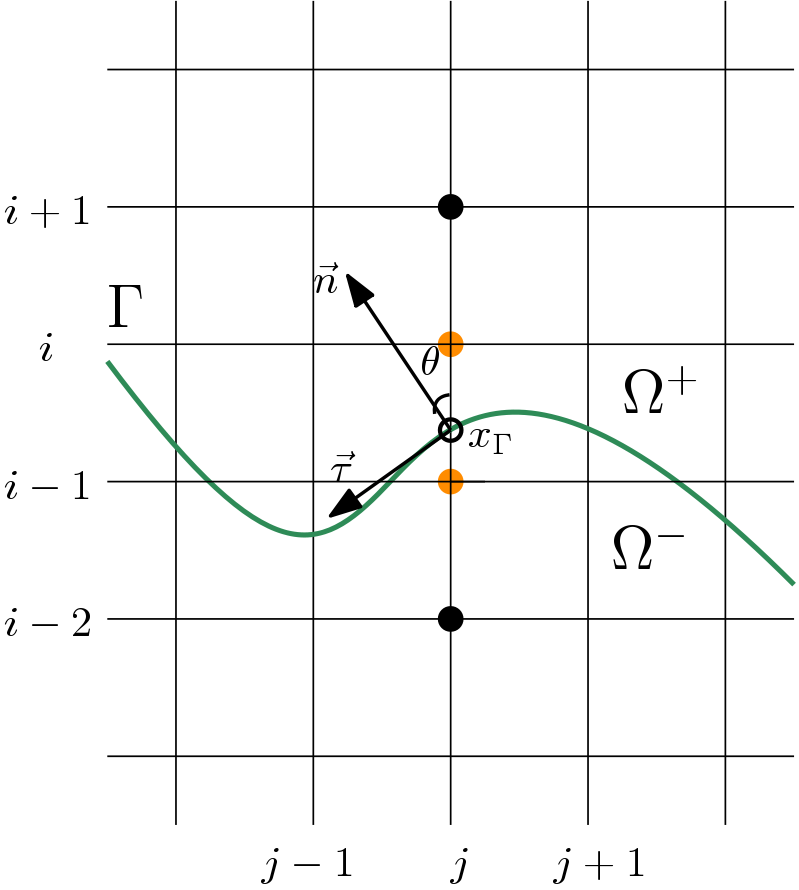
\includegraphics[width=7cm]{../figures/Irregular.png} & \quad & 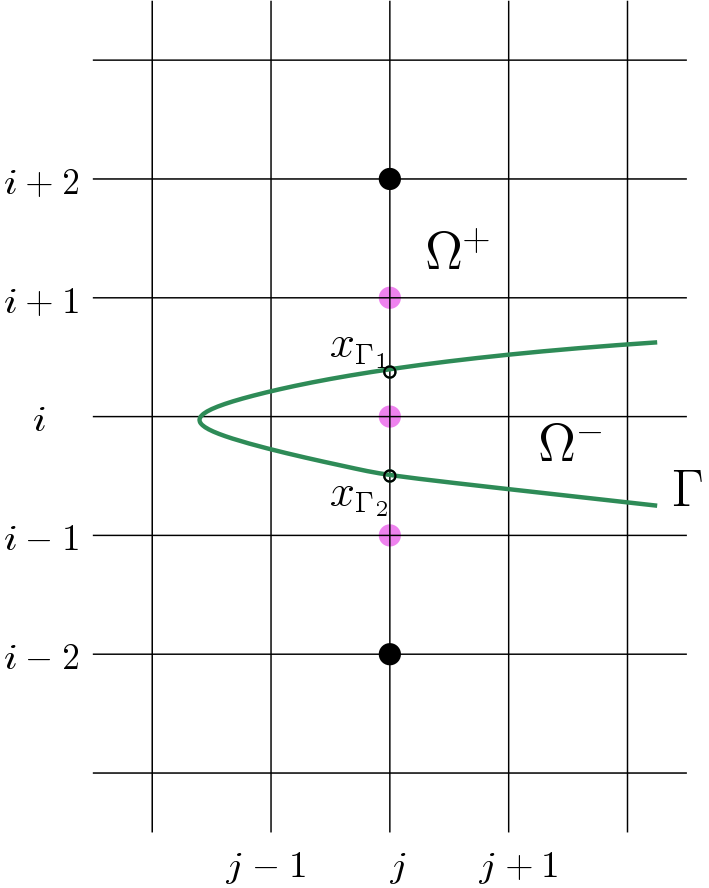
\includegraphics[width=7cm]{../figures/Corner_3.png} \\ 
				\ \textbf{(a)} & \quad & \textbf{(b)}
		\end{tabular}}
	\end{center}
	\caption{Three types of points: regular, irregular and corner point. 
		(a).Green curve is interface $\Gamma$ which separates $\Omega^{-}$ and $\Omega^{+}$, two orange nodes lies next to interface $\Gamma$ are called irregular points and the other two black nodes are regular points.
		(b).Green curve is still interface $\Gamma$ with high curvature, which separates inside sub-domain $\Omega^{-}$ and outside sub-domain $\Omega^{+}$. Three purple points next to interface $\Gamma$ are called corner points and the other two black nodes are regular points. }
	\label{fig:irregular and corner points_3}
\end{figure*}
%
\subsection{Ghost fluid method (GFM)}
In this work, we employ the Ghost Fluid method (GFM), to impose the interface condition (\ref{interface_jumps_3}) and correct formulas (\ref{delta_xx_3}) in each $x, y, z$ directions. A brief introduction to the GFM is provided below, more details could be referred to \cite{fedkiw1999non}. 

There are two major steps in GFM, first, in 2D case (see Fig.\ref{fig:irregular and corner points_3}(a)), decompose both the jump condition in normal direction $[\alpha u_n]$ and derived jump condition in tangential direction $[\alpha u_\tau]$ to $x, y$ directions, respectively, at each interface point. Assuming there is no jump condition along tangential direction, so that $[\alpha u_\tau] = 0$. The one can easily obtain  
%
\begin{equation}\label{GFM_jump_3}
[\alpha u_x] = cos\theta \cdot [\alpha u_n] = \psi_x, \quad [\alpha u_y] = sin\theta \cdot [\alpha u_n] = \psi_y, 
\end{equation}
%
where $\theta$ is the angle between normal direction $\vec{n}$ and $x$-axis. In three dimensional space, it follows the same manner to achieve $[\alpha u_x]$, $[\alpha u_y]$ and $[\alpha u_z]$ by assuming the derived jump conditions in two tangential directions $\eta$ and $\zeta$ both zero.

The second major step, is to utilize the jump conditions $[\alpha u_x]$, $[\alpha u_y]$ and $[\alpha u_z]$ to correct finite difference formulas at interface points. Considering $\delta^{\alpha}_{xx}$ as an example and still using Fig.\ref{fig:irregular and corner points_3}(a) to graphically  demonstrate the idea. To simplify the notations, we denote $x_\Gamma - x_{i-1} = \gamma \Delta x$ and thus $x_{i} - x_\Gamma = (1 - \gamma) \Delta x$, given variable diffusion coefficients as piecewise functions $\alpha^{-}(x,y,z)$ and $\alpha^{+}(x,y,z)$ in the two sub-domains $\Omega^{-}$ and $\Omega^{+}$, one can approximate $\alpha^{-}(u^{-}_{x})^{m+1}_{\Gamma}$ and $\alpha^{+}(u^{+}_{x})^{m+1}_{\Gamma}$ by
%
\begin{align}\label{GFM_interface_approximation_3}
\alpha^{-}(u^{-}_{x})^{m+1}_{\Gamma} = \alpha^{-}_{\Gamma}\frac{(u^{-})^{m+1}_{\Gamma} - 
	u^{m+1}_{i-1,j,k}}{\gamma \Delta x}, \quad
\alpha^{+}(u^{+}_{x})^{m+1}_{\Gamma} = \alpha^{+}_{\Gamma}\frac{u^{m+1}_{i,j,k} - 
	(u^{+})^{m+1}_{\Gamma}}{(1-\gamma)\Delta x}, 
\end{align}
%
at the interface point $x_\Gamma$ at time $t_{m+1}$ shown in Fig.\ref{fig:irregular and corner points_3}(a), and substitute into the jump conditions
%
\begin{align}
\label{GFM_jump_equation_1_3}
(u^{+})^{m+1}_{\Gamma} - (u^{-})^{m+1}_{\Gamma} = [u]^{m+1} &= \phi^{m+1}, \\
\label{GFM_jump_equation_2_3}
\alpha^{+} (u^{+}_x)^{m+1}_{\Gamma} - \alpha^{-}(u^{-}_x)^{m+1}_{\Gamma} = 
[\alpha u_x]^{m+1} &= \psi_x^{m+1}, 
\end{align}
%
solving for $(u^{-})^{m+1}_{\Gamma}$ and $(u^{+})^{m+1}_{\Gamma}$ as two unknown from the two equations. Accordingly, for the operator $\delta_{xx}^{\alpha}$ in $(\ref{delta_xx_3})$, to correct the finite difference scheme, an extrapolation of $(u^{+})^{m+1}_{\Gamma}$, $u^{m+1}_{i,j,k}$ and $u^{m+1}_{i+1,j,k}$ can be adopted to correct the value at node $(x_{i-1},y_j,z_k)$ in sub-domain $\Omega^{+}$, while the value at node $(x_i,y_j,z_k)$ in sub-domain $\Omega^{-}$ could be corrected by $(u^{-})^{m+1}_{\Gamma}$, $u^{m+1}_{i-1,j,k}$ and $u^{m+1}_{i-2,j,k}$.

\subsection{MIB-L1 method}
Even though the GFM provides a decent approximation to enforce jump conditions at interface point and delivers an accurate numerical solution, it is still negotiable whether the tangential jump conditions should be assumed to be trivial at the beginning. To address this concern, the new three-dimensional jump conditions decomposition technique introduced in section 2 can be carefully advocated in matched interface and boundary (MIB) method.

After decomposed the jump conditions into one-dimensional ones $[\alpha u_x]$, $[\alpha u_y]$ and $[\alpha u_z]$ using the technique we already discussed in section 3.1.3. Two kinds of point are introduced as regular point and irregular point, the difference of these two is the distance of grid point to interface, if a grid point is just next to the interface $\Gamma$ which means there is no other grid point between the point and interface, it is called an irregular point no matter which sub-domain they are in, otherwise, it is a regular point. As it is shown on Fig.\ref{fig:irregular and corner points_3}(a), both $u_{i,j,k}$, $u_{i-1,j,k}$ are irregular point and $u_{i+1,j,k}$ and $u_{i-2,j,k}$ are regular point. For regular point, the operators $\delta_{xx}^{\alpha}$, $\delta_{yy}^{\alpha}$ and $\delta_{zz}^{\alpha}$ are calculated from (\ref{delta_xx_3}), while in terms of irregular point, based on the sub-domain, a similar correction like GFM should be accomplished, 
$\delta_{xx}^{\alpha}$ is modified to be 
%
\begin{align}
\label{reformed_delta_xx_1}
\delta_{xx}^{\alpha} u^{m+1}_{i-1,j,k} &:=  
\frac{1}{\Delta x^{2}} ~ (\alpha^{-}_{i-\frac{3}{2},j,k} u^{m+1}_{i-2,j,k} - (\alpha^{-}_{i-\frac{3}{2},j,k} + \alpha^{-}_{i-\frac{1}{2},j,k}) u^{m+1}_{i-1,j,k} + \alpha^{-}_{i-\frac{1}{2},j,k} \tilde{u}^{m+1}_{i,j,k}), \\
\label{reformed_delta_xx_2}
\delta_{xx}^{\alpha} u^{m+1}_{i,j,k} &:=  
\frac{1}{\Delta x^{2}} ~ (\alpha^{+v}_{i-\frac{1}{2},j,k} \tilde{u}^{m+1}_{i-1,j,k} - (\alpha^{+}_{i-\frac{1}{2},j,k} + \alpha^{+}_{i+\frac{1}{2},j,k}) u^{m+1}_{i,j,k} + \alpha^{+}_{i+\frac{1}{2},j,k} u^{m+1}_{i+1,j,k}),
\end{align}
%
at the two irregular point $u_{i-1,j,k}$, $u_{i,j,k}$ at time $t_{m+1}$, where $\tilde u_{i-1,j,k}$ and $\tilde u_{i,j,k}$ are two fictitious values at node $(x_{i-1},y_j,z_k)$ and $(x_i,y_j,z_k)$, respectively, which are determined by discretizing two jump conditions in (\ref{GFM_jump_equation_1_3}) and (\ref{GFM_jump_equation_2_3}),
%
\begin{align}
\label{MIB_V1_jump_1_3}
\omega^{+}_{0,1}u_{i,j,k} + \omega^{+}_{0,2} \tilde{u}_{i-1,j,k} &=
\omega^{-}_{0,1} \tilde{u}_{i,j,k} + \omega^{-}_{0,2}u_{i-1,j,k} + \phi \\
\label{MIB_V2_jump_2_3} 
\alpha^{+}_{i,j,k}\omega^{+}_{1,1}u_{i,j,k}+\alpha^{+}_{i-1,j,k}\omega^{+}_{1,2}\tilde{u}_{i-1,j,k} &= 
\alpha^{-}_{i,j,k}\omega^{-}_{1,1}\tilde{u}_{i,j,k} + \alpha^{-}_{i-1,j,k}\omega^{-}_{1,2}u_{i-1,j,k} + \psi_{x}
\end{align}
%
where $\omega^{+}_{i,j}$ and $\omega^{-}_{i,j}$ are finite difference weights \cite{fornberg1998classroom} with $i=0$ representing interpolation and $i=1$ representing first order approximation. Solving (\ref{MIB_V1_jump_1_3}) and (\ref{MIB_V2_jump_2_3}) allow the two fictitious values $\tilde u_{i-1,j,k}$ and $\tilde u_{i,j,k}$ to be written as a linear combination of the two points $u_{i-1,j,k}$ and $u_{i,j,k}$ and two jump conditions $\phi$ and $\psi_x$. Due to the fact that $\psi_x$ is derived from jump conditions $[\alpha u_\xi]$, $[\alpha u_\eta]$ and $[\alpha u_\zeta]$ in (\ref{local-to-orginal_3}), the two fictitious values actually are written as a linear combinations of 
%
\begin{align}
\label{linear-combination-1_3}
\tilde{u}_{i-1,j,k} &= [a_0, a_1, a_2, a_3, a_4, a_5] \cdot [u_{i-1,j,k}, u_{i,j,k}, [u], [\alpha u_\eta], [\alpha u_\xi], [\alpha u_\zeta]]^{\intercal} \\
\label{linear-combination-2_3} 
\tilde{u}_{i,j,k} &= [b_0, b_1, b_2, b_3, b_4, b_5] \cdot [u_{i-1,j,k}, u_{i,j,k}, [u], [\alpha u_\eta], [\alpha u_\xi], [\alpha u_\zeta]]^{\intercal},
\end{align}
%
where all $a_i$ and $b_i$ are coefficients determined from solving (\ref{MIB_V1_jump_1_3}) and (\ref{MIB_V2_jump_2_3}). The fictitious value calculation is a time independent process, which is relatively cheap and only has to be performed once at the beginning of time iteration. Once all the coefficients $a_i$ and $b_i$ are attained, at each time step $t_{m+1}$, followed by a substitution of the two fictitious values, the correction of $\delta^{m+1}_{xx}$ is written as 
%
\begin{equation} 
\delta^{\alpha}_{xx} u^{m+1}_{i,j,k} = D^{\alpha}_{xx} u^{m+1}_{i,j,k} + B^{\alpha}_{x} u^{m}_{i,j,k} + \Phi_{x}^{m+1}, \label{delta_xx_operator_3}
\end{equation}
%
where $D^{\alpha}_{xx}$ is perturbed operators which have a band-width three at nodes $(x_i-1, y_j, z_k)$, $(x_i, y_j, z_k)$ and $(x_i+1, y_j, z_k)$. The operators $B^{\alpha}_{x}$ is due to tangential derivative approximations, which involves the value of point at previous time step $t_m$. The jump terms $\Phi^{m+1}_{x}$ is the sums of all jump conditions $[u]$, $[\alpha u_\eta]$, $[\alpha u_\xi]$, $[\alpha u_\zeta]$. The exact same idea will be adopted to $y$ and $z$ directions.

Despite of the jump conditions for $[\alpha u_x]$, $[\alpha u_y]$ and $[\alpha u_z]$, the MIB-L1 method is actually mathematical equivalent to the GFM, both employ the one-dimensional jump condition to correct the value of nodes around interface $\Gamma$ with locally first order. 

\subsection{MIB-L2 method}
Now, we introduce the second form of MIB method, MIB-L2 method, which inherit the same basic idea of MIB method but achieve a locally second order accuracy for nodes around interface. Similarly, to achieve second order accuracy to evaluate fictitious values, two more points at nodes $(x_{i-2},y_j,z_k)$ and $(x_{i+1},y_j,z_k)$ are immersed when discretizing the two jump conditions in (\ref{GFM_jump_equation_1_3}) and (\ref{GFM_jump_equation_2_3})
%
\begin{small}
	\begin{multline}
	\label{MIB_V2_fp_1_3}
	\omega^{+}_{0,1}u_{i+1,j,k} +
	\omega^{+}_{0,2}u_{i,j,k} +
	\omega^{+}_{0,3}\tilde{u}_{i-1,j,k} =
	\omega^{-}_{0,1}\tilde{u}_{i,j,k} +
	\omega^{-}_{0,2}u_{i-1,j,k} +
	\omega^{-}_{0,3}u_{i-2,j,k} +
	\phi,
	\end{multline}
	\begin{multline}
	\label{MIB_V2_fp_2_3}
	\lefteqn{\alpha^{+}_{i+1,j,k}\omega^{+}_{1,1}u_{i+1,j,k} +
		\alpha^{+}_{i,j,k}\omega^{+}_{1,2}u_{i,j,k} +
		\alpha^{+}_{i-1,j,k}\omega^{+}_{1,3}\tilde{u}_{i-1,j,k} =} \\ \alpha^{-}_{i,j,k}\omega^{-}_{1,1}\tilde{u}_{i,j,k} +
	\alpha^{-}_{i-1,j,k}\omega^{-}_{1,2}u_{i-1,j,k} +
	\alpha^{-}_{i-2,j,k}\omega^{-}_{1,3}u_{i-2,j,k} +
	\psi_{x}. 
	\end{multline}
\end{small}
%
After solving (\ref{MIB_V2_fp_1_3}) and (\ref{MIB_V2_fp_2_3}), $\tilde{u}_{i-1,j,k}$ and $\tilde{u}_{i,j,k}$ are written as linear combinations of 
%
\begin{align}
\label{linear-combination1_3}
\tilde{u}_{i-1,j,k} &= [a_0, a_1, a_2, a_3, a_4, a_5, a_6, a_7] \cdot [u_{i-2,j,k}, u_{i-1,j,k}, u_{i,j,k}, u_{i+1,j,k}, [u], [\alpha u_\eta], [\alpha u_\xi], [\alpha u_\zeta]]^{\intercal} \\
\label{linear-combination2_3} 
\tilde{u}_{i,j,k} &= [b_0, b_1, b_2, b_3, b_4, b_5, b_6, b_7] \cdot [u_{i-2,j,k}, u_{i-1,j,k}, u_{i,j,k}, u_{i+1,j,k}, [u], [\alpha u_\eta], [\alpha u_\xi], [\alpha u_\zeta]]^{\intercal},
\end{align}
%
where all $a_i$ and $b_i$ are still linear coefficients, which only need to be computed once before time iterations. To preserve second order accuracy in space, more situation has to be taken into consideration other than simply extend the scheme from MIB-L1 method. If the interface has a high curvature, see Fig.\ref{fig:irregular and corner points_3}(b), which make it really sharp or even non-smooth sometime, only one grid point will be found inside the region $\Omega^{-}$ no matter how dense the grid mesh is. It is called a corner case, and all the three points around the two side of the interfaces are called corner points. Three fictitious can be calculated located at the three corner points from four interface conditions at $x_{\Gamma_1}$ and $x_{\Gamma_2}$ in Fig.\ref{fig:irregular and corner points_3}(b) given by
%
\begin{small}
	\begin{multline}
	\label{MIB_V2_cp_1_3}
	\lefteqn{\omega^{+}_{0,1}u_{i+2,j,k} +
		\omega^{+}_{0,2}u_{i+1,j,k} +
		\omega^{+}_{0,3}\tilde{u}_{i,j,k} +
		\omega^{+}_{0,4}u_{i-1,j,k} =} \\
	\omega^{-}_{0,1}\tilde{u}_{i+1,j,k} +
	\omega^{-}_{0,2}u_{i,j,k} +
	\omega^{-}_{0,3}\tilde{u}_{i-1,j,k}+
	\omega^{-}_{0,4}\tilde{u}_{i-2,j,k} +
	\phi_{\Gamma_1},
	\end{multline}
	\begin{multline}
	\label{MIB_V2_cp_2_3}
	\lefteqn{\omega^{+}_{1,1}u_{i+2,j,k} +
		\omega^{+}_{1,2}u_{i+1,j,k} +
		\omega^{+}_{1,3}\tilde{u}_{i,j,k} +
		\omega^{+}_{1,4}u_{i-1,j,k} =} \\
	\omega^{-}_{1,1}\tilde{u}_{i+1,j,k} +
	\omega^{-}_{1,2}u_{i,j,k} +
	\omega^{-}_{1,3}\tilde{u}_{i-1,j,k}+
	\omega^{-}_{1,4}\tilde{u}_{i-2,j,k} +
	\phi_{\Gamma_2},
	\end{multline}
	\begin{multline}
	\label{MIB_V2_cp_3_3}
	\lefteqn{\alpha^{+}_{i+2,j,k}\omega^{+}_{2,1}u_{i+2.j,k} + 				  	\alpha^{+}_{i+1,j,k}\omega^{+}_{2,2}u_{i+1,j,k} + \alpha^{+}_{i,j,k}\omega^{+}_{2,3}\tilde{u}_{i,j,k} + \alpha^{+}_{i-1,j,k}\omega^{+}_{2,4}u_{i-1,j,k} =} \\ 
	\alpha^{-}_{i+1,j,k}\omega^{-}_{2,1}\tilde{u}_{i+1,j,k} 
	\alpha^{-}_{i,j,k}\omega^{-}_{2,2}u_{i,j,k} +
	\alpha^{-}_{i-1,j,k}\omega^{-}_{2,3}\tilde{u}_{i-1,j,k} +
	\alpha^{-}_{i-2,j,k}\omega^{-}_{2,4}\tilde{u}_{i-2,j,k} +
	\psi_{x_{\Gamma_1}}, 
	\end{multline}
	\begin{multline}
	\label{MIB_V2_cp_4_3}
	\lefteqn{\alpha^{+}_{i+2,j,k}\omega^{+}_{3,1}u_{i+2.j,k} + 			\alpha^{+}_{i+1,j,k}\omega^{+}_{3,2}u_{i+1,j,k} + \alpha^{+}_{i,j,k}\omega^{+}_{3,3}\tilde{u}_{i,j,k} + \alpha^{+}_{i-1,j,k}\omega^{+}_{3,4}u_{i-1,j,k} =} \\ 
	\alpha^{-}_{i+1,j,k}\omega^{-}_{3,1}\tilde{u}_{i+1,j,k} 
	\alpha^{-}_{i,j,k}\omega^{-}_{3,2}u_{i,j,k} +
	\alpha^{-}_{i-1,j,k}\omega^{-}_{3,3}\tilde{u}_{i-1,j,k} +
	\alpha^{-}_{i-2,j,k}\omega^{-}_{3,4}\tilde{u}_{i-2,j,k} +
	\psi_{x_{\Gamma_2}}. 
	\end{multline}
\end{small}

Note that there is one more extra fictitious values $\tilde{u}_{i-2,j,k}$ involved, since we would like to avoid extra degree of freedom, a non-degenerated matrix has to be constructed for solving the fictitious values. All the three fictitious values $\tilde{u}_{i-1,j,k}$, $\tilde{u}_{i,j,k}$ and $\tilde{u}_{i+1,j,k}$ will be eventually represented as a linear combination of all the five grid nodes $u_{i-2,j,k}$, $u_{i-1,j,k}$, $u_{i,j,k}$, $u_{i+1,j,k}$, $u_{i+2,j,k}$ and the four jump conditions $[u]$, $[\alpha u_\eta]$, $[\alpha u_\xi]$, $[\alpha u_\zeta]$ as (\ref{linear-combination1_3}) and (\ref{linear-combination2_3}).

A similar way can be performed in calculating fictitious values in $y$ and $z$ directions, afterward, at each time step $t_{m+1}$, one can just substitute related values of nodes for jump approximation at previous time step $t_m$ and required jump conditions at current time step $t_{m+1}$ to end up with the final forms of corrected operations 
%
\begin{eqnarray} 
\delta^{\alpha}_{xx} u^{m+1}_{i,j,k} &=& D^{\alpha}_{xx} u^{m+1}_{i,j,k} + B^{\alpha}_{x} u^{m}_{i,j,k} + \Phi_{x}^{m+1}, \label{delta_xx_operator_3} \\ 
\delta^{\alpha}_{yy} u^{m+1}_{i,j,k} &=& D^{\alpha}_{yy} u^{m+1}_{i,j,k} + B^{\alpha}_{y} u^{m}_{i,j,k} + \Phi_{y}^{m+1}, \label{delta_yy_operator_3} \\
\delta^{\alpha}_{zz} u^{m+1}_{i,j,k} &=& D^{\alpha}_{zz} u^{m+1}_{i,j,k} + B^{\alpha}_{z} u^{m}_{i,j,k} + \Phi_{z}^{m+1}, \label{delta_zz_operator_3},
\end{eqnarray}
%
where all node values at time step $t_{m+1}$ will be solved in the following time iterations and all node values at time step $t_m$ are provided from previous time step, meanwhile, all jump related operators $\Phi_{x}^{m+1}$, $\Phi_{y}^{m+1}$ and $\Phi_{z}^{m+1}$ are either derived or given from jump condition directly.

%%%%%%%%%%%%%%%%%%%%%%%%%%%%%%%%%%%%%%%%%%%%%%%%%%%%%%%%%%%%%%%%%%%%%%%%%%%%%%%%%%
\section{Operator splitting methods with variable coefficients}
During the recent decades, operator splitting methods has gained a lot of reputation for solving high-dimensional PDE problems, benifits from the efficiency and some unconditional stable property. These methods split the spatial dimensions and solve a 2D or 3D problem as two or three consecutive 1D problems. In the section we will introduce four different operator splitting methods Douglas-Rachford alternating direction implicit (D-ADI) method, Locally one-dimensional implicit Euler (LOD-IE) method, Locally one-dimensional Crank-Nicolson (LOD-CN) method and Trapezoidal Splitting (TS) method, respectively, and applied each to the original discretized equation (\ref{implicit_Euler_3}).

\subsection{Douglas-Rachford ADI scheme}
To construct a first order Douglas-Rachford ADI method \cite{douglas1955numerical2, paeceman1955numerical} based on the implicit Euler schemes of parabolic PDE (\ref{implicit_Euler_3}), at each grid point $(x_i, y_j, z_k)$ we rewrite (\ref{implicit_Euler_3}) as
%
\begin{align} \label{D_ADI_3}
(1-\Delta t \delta^{\alpha}_{xx}) u^{*}_{i,j,k}   &= (1 + \Delta t (\delta^{\alpha}_{yy} + \delta^{\alpha}_{zz})) u^{m}_{i,j,k} + \Delta t f^{m+1}_{i,j,k}, \nonumber \\
(1-\Delta t \delta^{\alpha}_{yy}) u^{**}_{i,j,k}  &= u^{*}_{i,j,k} - \Delta t \delta^{\alpha}_{yy} u^{m}_{i,j,k},  \\
(1-\Delta t \delta^{\alpha}_{zz}) u^{m+1}_{i,j,k} &= u^{**}_{i,j,k} - \Delta t \delta^{\alpha}_{zz} u^{m}_{i,j,k}, \nonumber
\end{align}
%
where the two terms $u^{*}_{i,j,k}$ and $u^{**}_{i,j,k}$ are intermediate terms. It's not hard to derive the similarity between Douglas-Rachford ADI scheme and the original implicit Euler scheme (\ref{implicit_Euler_3}) after dropping some higher order terms. The temporal order of Douglas-Rachford ADI method is the same with implicit Euler scheme, however, in respect of efficiency and computational cost, ADI is much faster then implicit Euler schemes with complexity $O(N)$, where $N$ is the total degree of freedom. The original left hand side matrix is not tridiagonal structure because of fictitious values, however, the non-tridiagonal parts are either 
$2\times4$ or $3\times5$ block matrices which can easily be simplified to tridiagonal structure by Gaussian elimination. The one-dimensional decomposition build up a tridiagonal matrix on the left hand side of the three equations (\ref{D_ADI_3}) which taking full advantages of Thomas algorithm. 

To deliver the optimal accuracy, jump condition corrections are imposed on the original implicit Euler scheme (\ref{implicit_Euler_3}) with MIB method, the original implicit Euler scheme (\ref{implicit_Euler_3}) are rewritten as  
%
\begin{equation} \label{implicit_Euler2_3}
\frac{u^{m+1}_{i,j,k}-u^{m}_{i,j,k}}{\Delta t} = 
D^{\alpha}_{xx} u^{m+1}_{i,j,k} +D^{\alpha}_{yy} u^{m+1}_{i,j,k} +D^{\alpha}_{zz} u^{m+1}_{i,j,k} + F^{m+1}_{i,j,k},
\end{equation}
%
where $F^{m+1}_{i,j,k}=(B^{\alpha}_{x}+B^{\alpha}_{y}+B^{\alpha}_{z})u^{m}_{i,j,k}+\Phi^{m+1}_{x}+\Phi^{m+1}_{y}+\Phi^{m+1}_{z}+f^{m+1}_{i,j,k}$. The Douglas-Rachford ADI method for the implicit Euler scheme \eqref{implicit_Euler2_3} is simply given as 
%
\begin{align} \label{D_ADI_2_3}
(1-\Delta t D^{\alpha}_{xx}) u^{*}_{i,j,k}   &= (1 + \Delta t (D^{\alpha}_{yy} + D^{\alpha}_{zz})) u^{m}_{i,j,k} + \Delta t F^{m+1}_{i,j,k}, \nonumber \\
(1-\Delta t D^{\alpha}_{yy}) u^{**}_{i,j,k}  &= u^{*}_{i,j,k} - \Delta t D^{\alpha}_{yy} u^{m}_{i,j,k},  \\
(1-\Delta t D^{\alpha}_{zz}) u^{m+1}_{i,j,k} &= u^{**}_{i,j,k} - \Delta t D^{\alpha}_{zz} u^{m}_{i,j,k}, \nonumber
\end{align}
%
which keep the semi-descretization and first temporal order, but more perturbation terms are eliminated in the proposed Douglas-Rachford ADI scheme from implicit Euler scheme. 

\subsection{Locally one-dimensional implicit Euler (LOD-IE) schemes}
The fractional step methods or locally one-dimensional (LOD) methods were first developed by Russian mathematicians \cite{yanenki1971lod}. Being multiplicative operator splitting methods too, the LOD methods adopt the similar splitting in alternating directions as in the ADI methods, but before the numerical discretization. we will formulate two types of temporal discretizations based on implicit Euler and Crank-Nicolson schemes. 

First, we propose the implicit Euler integration in time (\ref{implicit_Euler2_3}), decompose the three dimensional discretization form into three one-dimensional ones which leads to the LOD-IE scheme
%
\begin{align} \label{D_LODIE_3}
(1-\Delta t D^{\alpha}_{xx}) u^{*}_{i,j,k}   &= u^{m}_{i,j,k}, \nonumber \\
(1-\Delta t D^{\alpha}_{yy}) u^{**}_{i,j,k}  &= u^{*}_{i,j,k},  \\
(1-\Delta t D^{\alpha}_{zz}) u^{***}_{i,j,k} &= u^{**}_{i,j,k}, \nonumber \\
u^{m+1}_{i,j,k} &= u^{***}_{i,j,k} + \Delta t F^{m+1}_{i,j,k},
\end{align}
%
where all operators $D^{\alpha}_{xx}$, $D^{\alpha}_{xx}$, $D^{\alpha}_{xx}$ and source term $F^{m+1}_{i,j,k}$ has been corrected for nodes near interface $\Gamma$ spatially. The LOD-IE scheme has exact same right hand side with Douglas-Rachford ADI scheme (\ref{D_ADI_2_3}) but a simplified left hand side, therefore, it keep the unconditional stability property but less operations are expected in the computation.

\subsection{Locally one-dimensional Crank-Nicolson (LOD-CN) schemes}
Minor change can be resulted if we consider a well known Crank-Nicolson integration in time based on governing equation (\ref{heat_eqn_3}) with corrected operators in all three directions, 
%
\begin{equation} \label{Crank-Nicolson_3}
\frac{u^{m+1}_{i,j,k}-u^{m}_{i,j,k}}{\Delta t} = 
\frac{1}{2}(D^{\alpha}_{xx} u^{m}_{i,j,k} + D^{\alpha}_{xx} u^{m+1}_{i,j,k} + D^{\alpha}_{yy} u^{m}_{i,j,k} + D^{\alpha}_{yy} u^{m+1}_{i,j,k} + D^{\alpha}_{zz} u^{m}_{i,j,k} + D^{\alpha}_{zz} u^{m+1}_{i,j,k} + F^{m}_{i,j,k} + F^{m+1}_{i,j,k}),
\end{equation}
%
Utilizing locally one dimensional scheme based on (\ref{Crank-Nicolson_3}) leads to
%
\begin{align} \label{D_LODCN_3}
(1-\frac{\Delta t}{2} D^{\alpha}_{xx}) u^{*}_{i,j,k}   &= (1+\frac{\Delta t}{2} D^{\alpha}_{xx})u^{m}_{i,j,k}, \nonumber \\
(1-\frac{\Delta t}{2} D^{\alpha}_{yy}) u^{**}_{i,j,k}  &= (1+\frac{\Delta t}{2} D^{\alpha}_{xx})u^{*}_{i,j,k},  \\
(1-\frac{\Delta t}{2} D^{\alpha}_{zz}) u^{***}_{i,j,k} &= (1+\frac{\Delta t}{2} D^{\alpha}_{xx})u^{**}_{i,j,k}, \nonumber \\
u^{m+1}_{i,j,k} &= u^{***}_{i,j,k} + \frac{1}{2} (\Delta t F^{m+1}_{i,j,k} + \Delta t F^{m}_{i,j,k}).
\end{align}
%
One may think the scheme is second-order in time, nonetheless, because the jump approximation is only first order accuracy, the scheme still keep first order in time. Fortunately, unconditional stable is still well preserved on this LOD-CN scheme. 

\subsection{Trapezoidal Splitting (TS) schemes}
Inspired by \cite{hundsdorfer1998trapezoidal} about trapezoidal splitting, one splitting method which is based on the trapezoidal rule,
%
\begin{equation} \label{Trapezoidal_rule_3}
u^{m+1} = u^{m} + \frac{1}{2} \Delta t G(t_m, u^m) + \frac{1}{2} \Delta t G(t_{m+1}, u^{m+1}), 
\end{equation}
%
where the function $G$ can be treated as the entire right hand side of the governing equation (\ref{heat_eqn_3}). There are three direction and source term involved in the governing equation, it is possible to decompose the function $G$ into four simpler component functions, 
%
\begin{equation} \label{decompose_G_3}
G(t, u) = G_1(t, u) + G_2(t, u) + G_3(t, u) + G_4(t, u), 
\end{equation}
%
where $G_1$, $G_2$, $G_3$ are indeed the corrected operators $D^{\alpha}_{xx}$, $D^{\alpha}_{yy}$, $D^{\alpha}_{zz}$ and $G_4$ is the source term $F$, which ultimately leads to a large set of system of equations
%
\begin{align} \label{TS_3}
v^{(1)}_{i,j,k} &= (1+\frac{\Delta t}{2} D^{\alpha}_{xx})u^{m}_{i,j,k}, \nonumber \\
v^{(2)}_{i,j,k} &= (1+\frac{\Delta t}{2} D^{\alpha}_{yy})v^{(1)}_{i,j,k}, \nonumber \\
v^{(3)}_{i,j,k} &= (1+\frac{\Delta t}{2} D^{\alpha}_{zz})v^{(2)}_{i,j,k}, \nonumber \\
v^{(4)}_{i,j,k} &= v^{(3)}_{i,j,k} + \frac{\Delta t}{2} F^{m}_{i,j,k}(v^{(3)}), \nonumber \\
v^{(5)}_{i,j,k} &= v^{(4)}_{i,j,k} + \frac{\Delta t}{2} F^{m+1}_{i,j,k}(v^{(4)}), \\
(1-\frac{\Delta t}{2} D^{\alpha}_{zz})v^{(6)}_{i,j,k} &= v^{(5)}_{i,j,k}, \nonumber \\
(1-\frac{\Delta t}{2} D^{\alpha}_{yy})v^{(7)}_{i,j,k} &= v^{(6)}_{i,j,k}, \nonumber \\
(1-\frac{\Delta t}{2} D^{\alpha}_{xx})u^{m+1}_{i,j,k} &= v^{(7)}_{i,j,k}. \nonumber
\end{align}
%
as the trapezoidal splitting method with corrected operators. One may notice that the system is not entirely symmetric due to the fifth equation in (\ref{TS_3}), which is because of the efficiency reason. To take a symmetric form in the fifth equation of (\ref{TS_3}), source term $F^{m+1}_{i,j,k}(v^{(4)})$ has to be replaced by $F^{m+1}_{i,j,k}(v^{(5)})$. Therefore, when derived jump conditions will involve an implicitly part represented $(B^{\alpha}_{x}+B^{\alpha}_{y}+B^{\alpha}_{z})v^{5}_{i,j,k}$, which should move to the left hand side to solve the equation, the matrix structure will be detracted from a tridiagonal matrix and has to be solved by some expensive iterative algorithm instead of Thomas algorithm with $O(N)$.

In the computations, all boundary conditions are Dirichlet boundary conditions which assumed to be at the next time step $t_{m+1}$ when calculating the intermediate terms. If more than first order of accuracy is considered in space, technique \cite{zhao2009matched} using MIB method in high order central finite difference can be utilized.


%----------------------------------------------------------------------%
%                                                                      %
%                             Chapter 4                                %
%                                                                      %
%----------------------------------------------------------------------%
\chapter{\MakeUppercase{Numerical experiments}}

The numerical performance of all proposed methods is measured by two error measurements, $L_{\infty}$ and $L_2$ norms, which are defined as 
\begin{align}
L_{\infty} &= \max_{i,j,k} \mid u(x_{i},y_{j},z_{k}) - u_h(x_{i},y_{j},z_{k})\mid,  \\
L_2 &= \sqrt{\frac{\sum_{i,j,k} (u(x_{i},y_{j},z_{k}) - u_h(x_{i},y_{j},z_{k}))^2}{N_{x}*N_{y}*N_{z}}}.
\end{align}
where $u_h(x_{i},y_{j},z_{k})$ is the numerical solution, and
$N_{x}$, $N_{y}$ and $N_{z}$ represent the numbers of grid nodes on $x$, $y$ and $z$ direction. The order of convergence for both $L_2$ and $L_{\infty}$ is reported in all tested cases. For the surface solution and error maps, the values on the interface points are mapped by the closest grid node from exterior sub-domain $\Omega^{+}$, and the numbers of mesh grid are chosen to be large so that the exterior value of the surface will be extremely close to its closest outside nodal value.

To better understand the implementation in three dimensional space, a visualization of sphere is proposed to illustrate the finite different process in Fig. \ref{fig:Implementation}. For other surface we used in numerical experiments, the idea is the same.
%
\begin{figure*}[!tb] 
	\begin{center}
		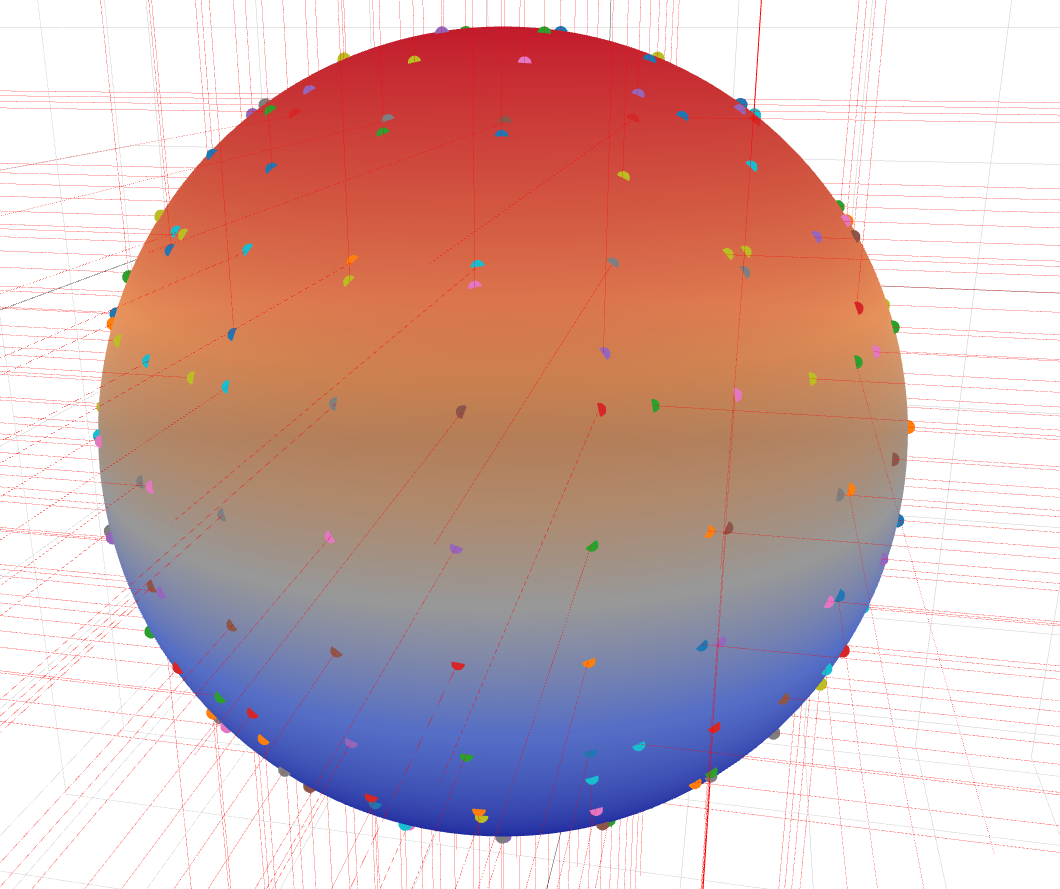
\includegraphics[width=13cm]{../figures/nodes.png}
	\end{center}
	\caption{Implementation illustration based on finited difference in three dimensional space. The surface $\Gamma$ is a sphere, which separate the two subdomains. In three dimensional space, a straight line cuts through the entire domain $\Omega$ at each grid point in each direction, which intersects the surface at some arbitrary node.}
	\label{fig:Implementation}
\end{figure*}
%

\section{Matched ADI with constant piece-wise coefficients}
In this section, we examine both temporal and spatial convergence rates of the proposed 3D matched ADI algorithm with various shapes of interfaces and jump conditions. The code is written in C++ based on the idea of objected oriented programming. The data structure ``vector'' in C++ STL is selected to perform the linked-list feature. With such a new data structure, the grid line can cross the interface many times without restriction, while in our previous 2D matched ADI methods \cite{zhao2015matched,li2017matched}, it allowed to cross at most twice. The present data structure enables us to treat more complicated geometry in 3D. Reported CPU time is recorded on the master node of SGI Ultraviolet in Alabama Supercomputer Center with a single Xeon E5-4640 CPU core operating at 2.4 GHz clock speed. 

In all examples, a piecewisely defined analytical solution $u(x,y,z)$ is constructed so that both the initial condition at time $t=0$ and Dirichlet boundary conditions on the boundary of a cubic computational domain $\Omega$ can be obtained from the constructed analytical solution directly.
 
Unless specified individually, the integration will be carried out until a stopping time $t=1$ and the diffusion coefficients are selected as $\alpha^{-}=1$ and $\alpha^{+}=10$. 
The domain size is chosen as a non-integer so that one can avoid the situation, in which
the interface intersects the Cartesian grid lines through one grid node,
because  such a situation rarely happens for a complex geometry in practice. 
Moreover, by taking the domain size very close to an integer, such as 1.99, 
the corner interface case could be encountered in a coarse mesh. 
This enables us to fully validate the proposed matched ADI algorithm.

%----------------------------------------------------------------------%
%                                                                      %
%                               Example 1                              %
%                                                                      %
%----------------------------------------------------------------------%
{\flushleft \bf Example 1.} The first example has a simple smooth ellipsoid surface, which is defined as the zero level set of
% 
\begin{equation} \label{ellipsoid}
S(x,y,z) = \frac{x^{2}}{4} + y^{2} + z^{2} -1.
\end{equation}
%
This interface is regular and convex so that each grid line cuts the interface at most twice. The analytical solution to eqn. (\ref{heat_eqn}) is constructed to be
%
\begin{equation} \label{analytical_eqn_1}
u(x,y,z,t)= 
\begin{cases}
10e^{-x^{2}}e^{-y^{2}}e^{-z^{2}}-e^{t-a}, \quad   &\mbox{in } \Omega^{-} \\
5e^{-x^{2}}e^{-y^{2}}e^{-z^{2}}+e^{t-a},  \quad   &\mbox{in } \Omega^{+}
\end{cases}
\end{equation}
%
with $a=2$. The source term is
%
\begin{equation} \label{source_eqn_1}
f(x,y,z,t)= 
\begin{cases}
-10 \alpha^{-} (-6+4(x^{2}+y^{2}+z^{2})) e^{-x^{2}}e^{-y^{2}}e^{-z^{2}} - e^{t-a}, \quad   &\mbox{in } \Omega^{-} \\
-5 \alpha^{+} (-6+4(x^{2}+y^{2}+z^{2})) e^{-x^{2}}e^{-y^{2}}e^{-z^{2}} + e^{t-a}.  \quad   &\mbox{in } \Omega^{+},
\end{cases}
\end{equation}
%
so that the zeroth order jump condition on the interface is time-dependent, while the first order jump condition is time-independent. The computational domain is fixed to be  $[-3.99,3.99]\times[-1.99,1.99]\times[-1.99,1.99]$. 

The proposed matched ADI algorithm is stable and
convergent for all tested combinations of $h$ and $\Delta t$. In order to demonstrate the spatial convergence rate, $\Delta t = 10^{-4}$ is set to be small. Numerical results obtained by varying the number of grids per direction are demonstrated in Table \ref{table:ellipsoid}, and it is obvious that the spatial convergence rate is close to 2 for both $L_{\infty}$ and $L_2$ norms. 
%
%\noindent
\begin{table}
	\centering
	\renewcommand{\arraystretch}{1.0}% Tighter
	\resizebox{\textwidth}{!}{
		\tiny
		\begin{tabular}{c @{\hskip 8mm} cccccccc @{}}\midrule
			\multirow{2}{*}{$[N_{x},N_{y},N_{z}]$} 
			&\multicolumn{2}{c}{$L_{\infty}$}  & \phantom{abc} &\multicolumn{2}{c}{$L_2$} \\ 
			\cmidrule{2-3} \cmidrule{5-6}
			&\multicolumn{1}{c}{Error}  &\multicolumn{1}{c}{Order}  & \phantom{abc} 
			&\multicolumn{1}{c}{Error}  &\multicolumn{1}{c}{Order} \\
			\hline
			$[20,20,20]$      & 1.507e-01  &        & & 2.016e-02  &      \\
			$[40,40,40]$      & 4.521e-02  & 1.74   & & 4.324e-03  & 2.22 \\
			$[80,80,80]$      & 9.833e-03  & 2.20   & & 1.288e-03  & 1.75 \\
			$[160,160,160]$   & 2.187e-03  & 2.17   & & 3.743e-04  & 1.78 \\
			\hline
		\end{tabular}
	}
	\captionof{table}{Spatial convergence for ellipsoid surface.}
	\label{table:ellipsoid}
\end{table}
%
%
\begin{figure*}[!tb] 
	\begin{center}
		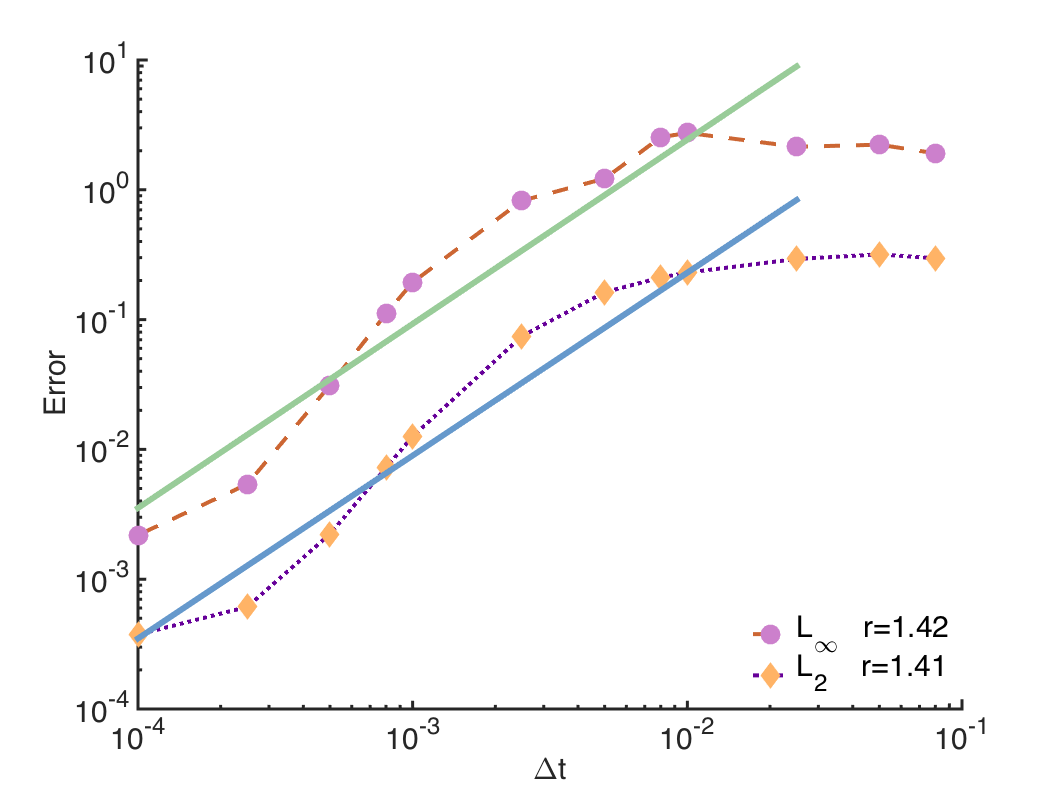
\includegraphics[width=12cm]{../figures/Ellipsoid_Time.png}
	\end{center}
	\caption{Temporal convergence for ellipsoid surface.}
	\label{fig:temporal_convergence_ellipsoid}
\end{figure*}
%
The next set of tests is performed with a dense space mesh $[N_{x},N_{y},N_{z}]=[160,160,160]$, and various time steps. The results are depicted in Fig. \ref{fig:temporal_convergence_ellipsoid} with dashed lines. 
One can observe that the convergence is not evident for  $\Delta t > 10^{-2}$,
probably because of the relatively large errors in approximating tangential derivatives for a large $\Delta t$. Once the convergence starts at $\Delta t=10^{-2}$, the rate is pretty high. To see this,  a least-squares fitting \cite{zhao2009matched} is conducted in the log-log scale to analyze the temporal convergence rate, which is demonstrated by the solid lines in Figure \ref{fig:temporal_convergence_ellipsoid}. Their slopes shown in the legend of 
Figure \ref{fig:temporal_convergence_ellipsoid}
represent the temporal convergence rate of the scheme. It shows that both solid lines for $L_2$ and $L_{\infty}$ errors have slopes about $40\%$ higher than their theoretical orders (one). 

The color maps of numerical solutions and errors of Example 1 are depicted in Fig. \ref{fig:color_map_ellipsoid} for  $[N_{x},N_{y},N_{z}]=[160,160,160]$ and $\Delta t=10^{-4}$. It is found that large errors occur in the places where the solutions have large magnitudes. This is natural due to the simple shape of the ellipsoid surface.  

\begin{figure*}[!ht]	
	\begin{center}
		\resizebox{\textwidth}{!}{
			\begin{tabular}{ccc}
				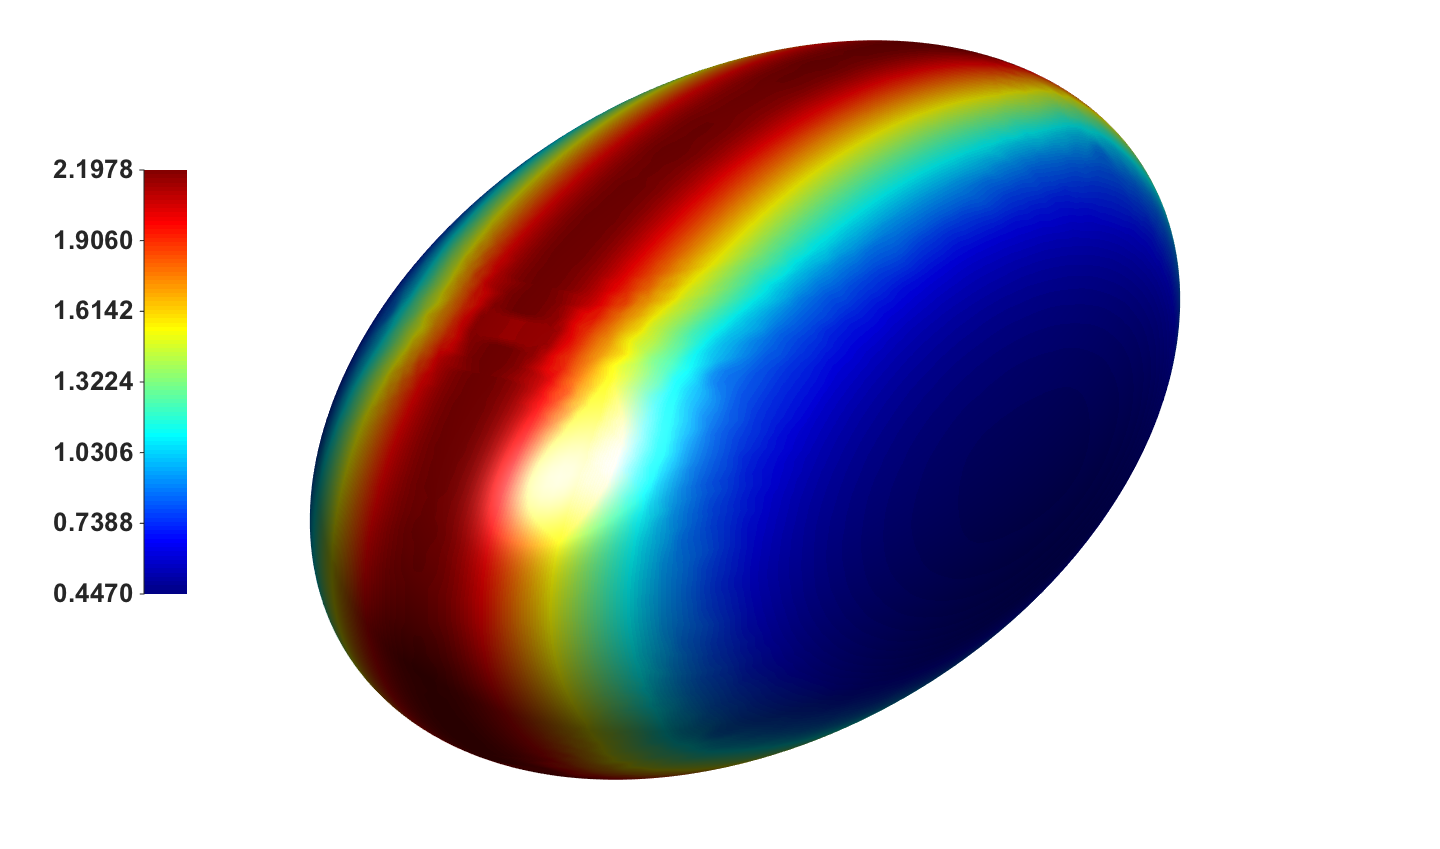
\includegraphics[width=10cm]{../figures/Ellipsoid_Solution.png} & \quad & 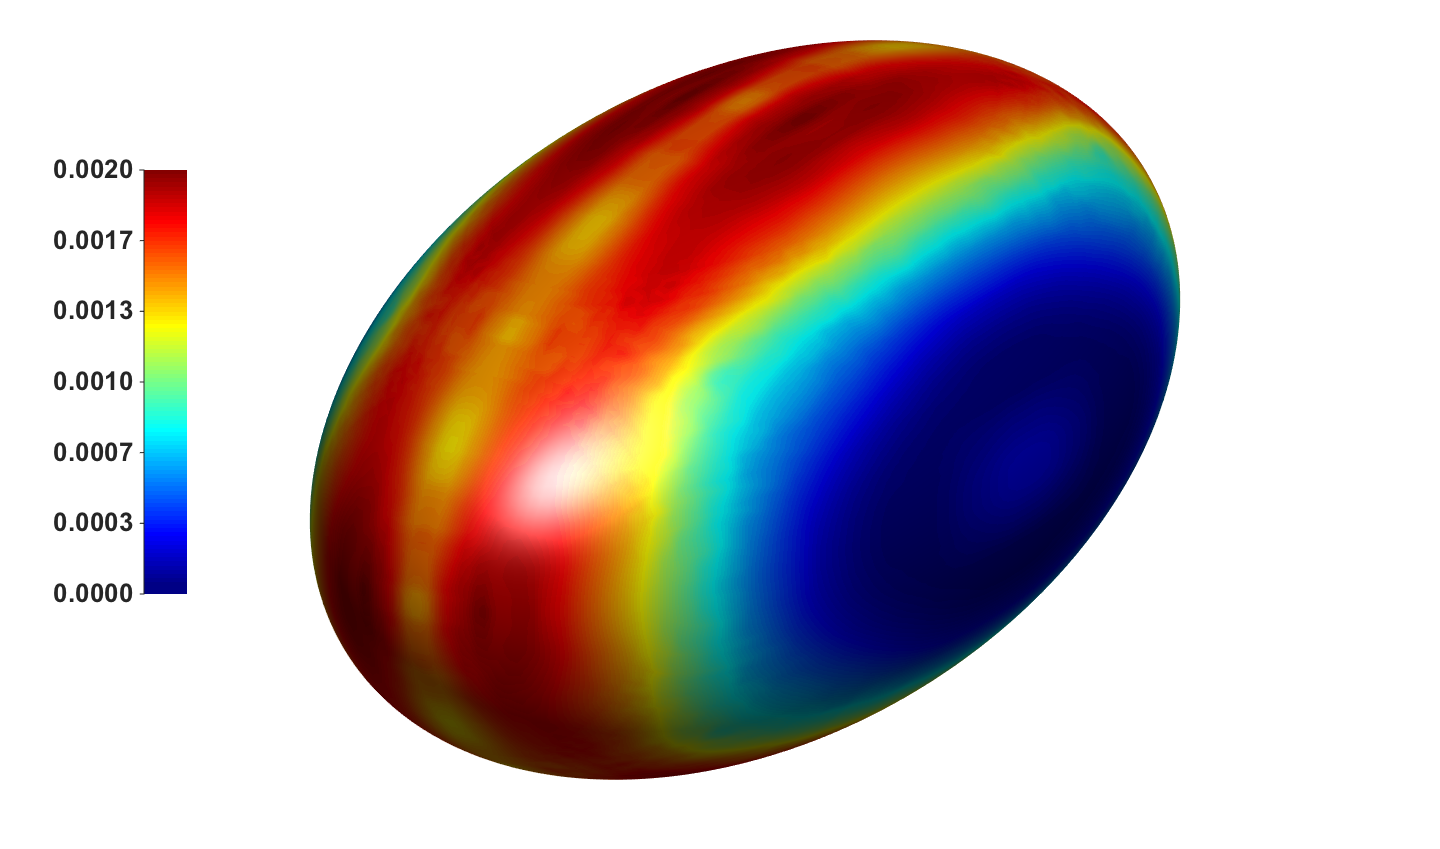
\includegraphics[width=10cm]{../figures/Ellipsoid_Error.png} \\ 
				\textbf{(a)} & \quad & \textbf{(b)}
		\end{tabular}}
	\end{center}
	\caption{Color maps for ellipsoid surface. (a). numerical solution; (b). numerical error.}
	\label{fig:color_map_ellipsoid}
\end{figure*} 
%

%----------------------------------------------------------------------%
%                                                                      %
%                               Example 2                              %
%                                                                      %
%----------------------------------------------------------------------%

{\flushleft \bf Example 2.} The second example has a simple cylinder surface, which is defined as an implicit function
% 
\begin{equation} \label{cylinder_eq}
\frac{x^{2}}{4}+\frac{y^{2}}{4}=1 , \quad -3\leqslant z \leqslant3. \\
\end{equation}
%
In two-dimensional views, this interface is either a rectangle or a circle. 
%This interface is relatively easy and the shapes are either rectangle or circle in a two-dimensional view. 
The same analytical solution \eqref{analytical_eqn_1} and source term \eqref{source_eqn_1} with $a=1$ as in 
Example 1 are studied. 
The computational domain is fixed to be $[-3.99,3.99]\times[-3.99,3.99]\times[-3.99,3.99]$.

We are interested in studying different combinations for the diffusion coefficients for this example. 
Besides the usual combination with $(\alpha^{-},\alpha^{+})=(1,10)$, two more cases with $(\alpha^{-},\alpha^{+})=(10,1)$ and $(\alpha^{-},\alpha^{+})=(1,100)$ are examined. 
The 3D matched ADI method is found to be stable for all the tested $h$ and $\Delta t$ 
for these three pairs of diffusion coefficients. 
From Table \ref{table:cylinder_1_10} to Table \ref{table:cylinder_1_100}, to avoid the influence of temporal numerical errors, a small fixed time increment $\Delta t=10^{-4}$ is adopted for all spatial convergence tests. The results of all three tables indicate that both $L_2$ and $L_{\infty}$ norms achieve second order convergence rate regardless of the diffusion coefficient's combinations. 
By fixing the number of grids in each direction to be 160,
the temporal convergence is investigated by
the least-square fitting analysis
in Figure \ref{fig:temporal_convergence_cylinder_1_10} to \ref{fig:temporal_convergence_cylinder_1_100}.
It is clear that $L_2$ and $L_{\infty}$ errors yield a similar behavior, and both converge at 
a rate slightly higher than the first order. 

%
%\noindent
\begin{table}
	\centering
	\renewcommand{\arraystretch}{1.0}% Tighter
	\resizebox{\textwidth}{!}{
		\tiny
		\begin{tabular}{c @{\hskip 8mm} cccccccc @{}}\midrule
			\multirow{2}{*}{$[N_{x},N_{y},N_{z}]$} 
			&\multicolumn{2}{c}{$L_{\infty}$}  & \phantom{abc} &\multicolumn{2}{c}{$L_2$} \\ 
			\cmidrule{2-3} \cmidrule{5-6}
			&\multicolumn{1}{c}{Error}  &\multicolumn{1}{c}{Order}  & \phantom{abc} 
			&\multicolumn{1}{c}{Error}  &\multicolumn{1}{c}{Order} \\
			\hline
			$[20,20,20]$      & 4.548e-01  &        & & 2.262e-02  &      \\
			$[40,40,40]$      & 1.215e-01  & 1.90   & & 5.122e-03  & 2.14 \\
			$[80,80,80]$      & 3.020e-02  & 2.00   & & 1.227e-03  & 2.06 \\
			$[160,160,160]$   & 7.491e-03  & 2.11   & & 3.035e-04  & 2.02 \\
			\hline
	\end{tabular}}
	\captionof{table}{Spatial convergence for cylinder surface with $\alpha^{-}=1$ and $\alpha^{+}=10$.}
	\label{table:cylinder_1_10}
\end{table}
%
%
\begin{figure*}[!tb] 
	\centering
	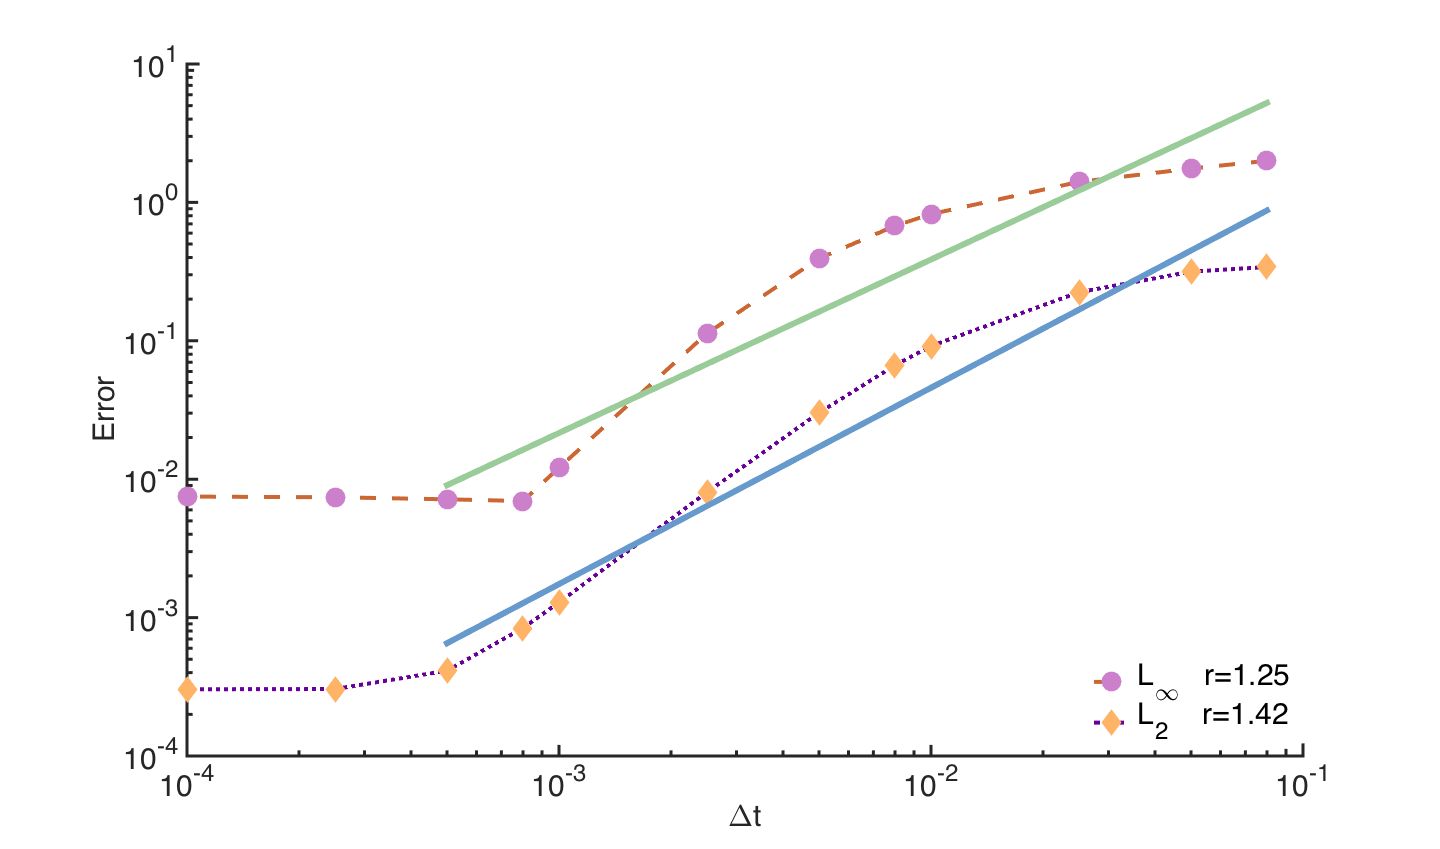
\includegraphics[width=13cm]{../figures/Cylinder_Time_1&10.png}
	\captionof{figure}{Temporal convergence for cylinder surface with $\alpha^{-}=1$ and $\alpha^{+}=10$.}
	\label{fig:temporal_convergence_cylinder_1_10}
\end{figure*}
%
%
%\noindent
\begin{table}
	\centering
	\renewcommand{\arraystretch}{1.0}% Tighter
	\resizebox{\textwidth}{!}{
		\tiny
		\begin{tabular}{c @{\hskip 8mm} cccccccc @{}}\midrule
			\multirow{2}{*}{$[N_{x},N_{y},N_{z}]$} 
			&\multicolumn{2}{c}{$L_{\infty}$}  & \phantom{abc} &\multicolumn{2}{c}{$L_2$} \\ 
			\cmidrule{2-3} \cmidrule{5-6}
			&\multicolumn{1}{c}{Error}  &\multicolumn{1}{c}{Order}  & \phantom{abc} 
			&\multicolumn{1}{c}{Error}  &\multicolumn{1}{c}{Order} \\
			\hline
			$[20,20,20]$      & 5.271e-01  &        & & 3.802e-02  &      \\
			$[40,40,40]$      & 1.074e-01  & 2.30   & & 7.891e-03  & 2.27 \\
			$[80,80,80]$      & 2.571e-02  & 2.06   & & 2.388e-03  & 1.72 \\
			$[160,160,160]$   & 6.788e-03  & 1.92   & & 4.558e-04  & 2.39 \\
			\hline
	\end{tabular}}
	\captionof{table}{Spatial convergence for cylinder surface with $\alpha^{-}=10$ and $\alpha^{+}=1$.}
	\label{table:cylinder_10_1}
\end{table}
%
%
\begin{figure*}[!tb] 
	\centering
	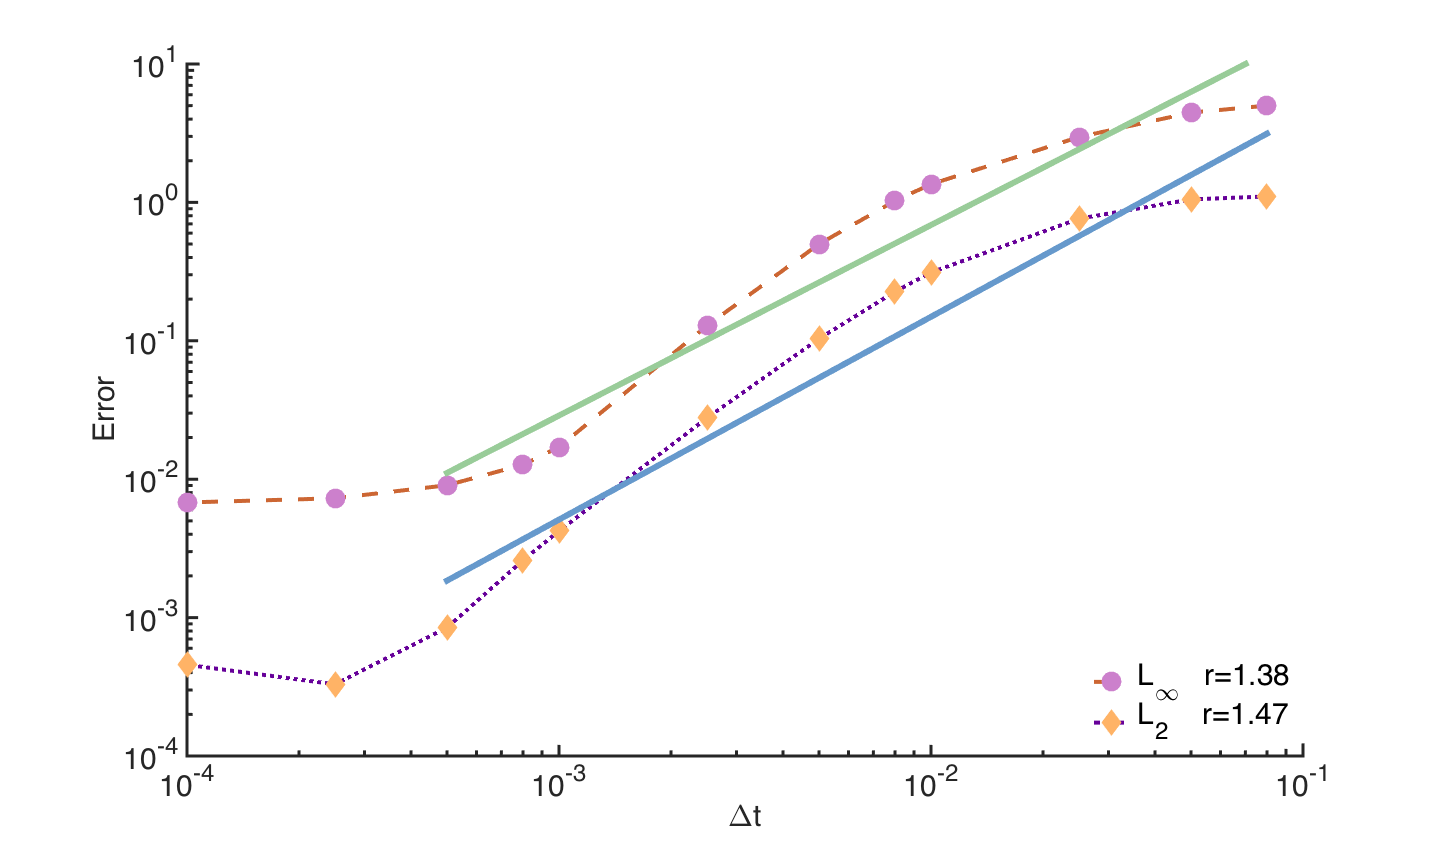
\includegraphics[width=13cm]{../figures/Cylinder_Time_10&1.png}
	\captionof{figure}{Temporal convergence for cylinder surface with $\alpha^{-}=10$ and $\alpha^{+}=1$.}
	\label{fig:temporal_convergence_cylinder_10_1}
\end{figure*}
%
%
%\noindent
\begin{table}
	\centering
	\renewcommand{\arraystretch}{1.0}% Tighter
	\resizebox{\textwidth}{!}{
		\tiny
		\begin{tabular}{c @{\hskip 8mm} cccccccc @{}}\midrule
			\multirow{2}{*}{$[N_{x},N_{y},N_{z}]$} 
			&\multicolumn{2}{c}{$L_{\infty}$}  & \phantom{abc} &\multicolumn{2}{c}{$L_2$} \\ 
			\cmidrule{2-3} \cmidrule{5-6}
			&\multicolumn{1}{c}{Error}  &\multicolumn{1}{c}{Order}  & \phantom{abc} 
			&\multicolumn{1}{c}{Error}  &\multicolumn{1}{c}{Order} \\
			\hline
			$[20,20,20]$      & 4.562e-01  &        & & 2.275e-02  &      \\
			$[40,40,40]$      & 1.224e-01  & 1.90   & & 5.241e-03  & 2.12 \\
			$[80,80,80]$      & 3.038e-02  & 2.01   & & 1.243e-03  & 2.08 \\
			$[160,160,160]$   & 7.525e-03  & 2.01   & & 3.058e-04  & 2.02 \\
			\hline
	\end{tabular}}
	\captionof{table}{Spatial convergence for cylinder surface with $\alpha^{-}=1$ and $\alpha^{+}=100$.}
	\label{table:cylinder_1_100}
\end{table}
%
%
\begin{figure*}[!tb] 
	\centering
	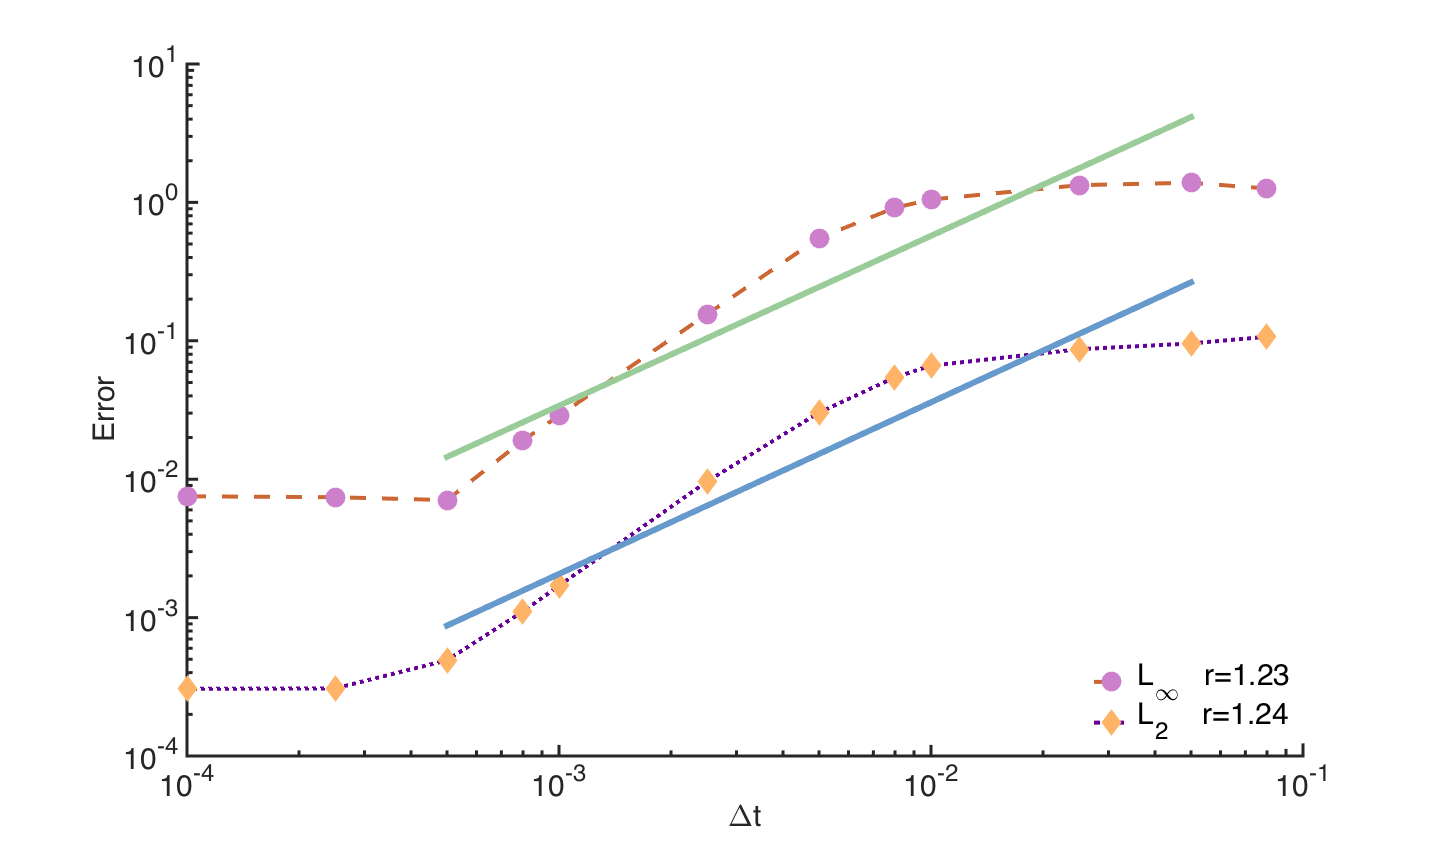
\includegraphics[width=13cm]{../figures/Cylinder_Time_1&100.png}
	\captionof{figure}{Temporal convergence for cylinder surface with $\alpha^{-}=1$ and $\alpha^{+}=100$.}
	\label{fig:temporal_convergence_cylinder_1_100}
\end{figure*}
%

%----------------------------------------------------------------------%
%                                                                      %
%                               Example 3                              %
%                                                                      %
%----------------------------------------------------------------------%

{\flushleft \bf Example 3.} The third example studies the impact of the curvature of the interface on the proposed numerical scheme. To this end, a smooth molecular surface of two atoms is constructed by the zero level set of 
%
\begin{equation}
S(x,y,z) = (x^{2}+y^{2}+z^{2}+\frac{3}{5})^2 -\frac{7}{2}y^{2} - \frac{3}{5}
\end{equation}
%
within a cubic computational domain $\Omega$ of dimension $[-1.99,1.99]\times[-2.99,2.99]\times[-1.99,1.99]$, as shown in Figure \ref{fig:color_map_molecular}. 
%
\begin{figure*}[!ht]
	\begin{center}
		\resizebox{\textwidth}{!}{
			\begin{tabular}{ccc}
				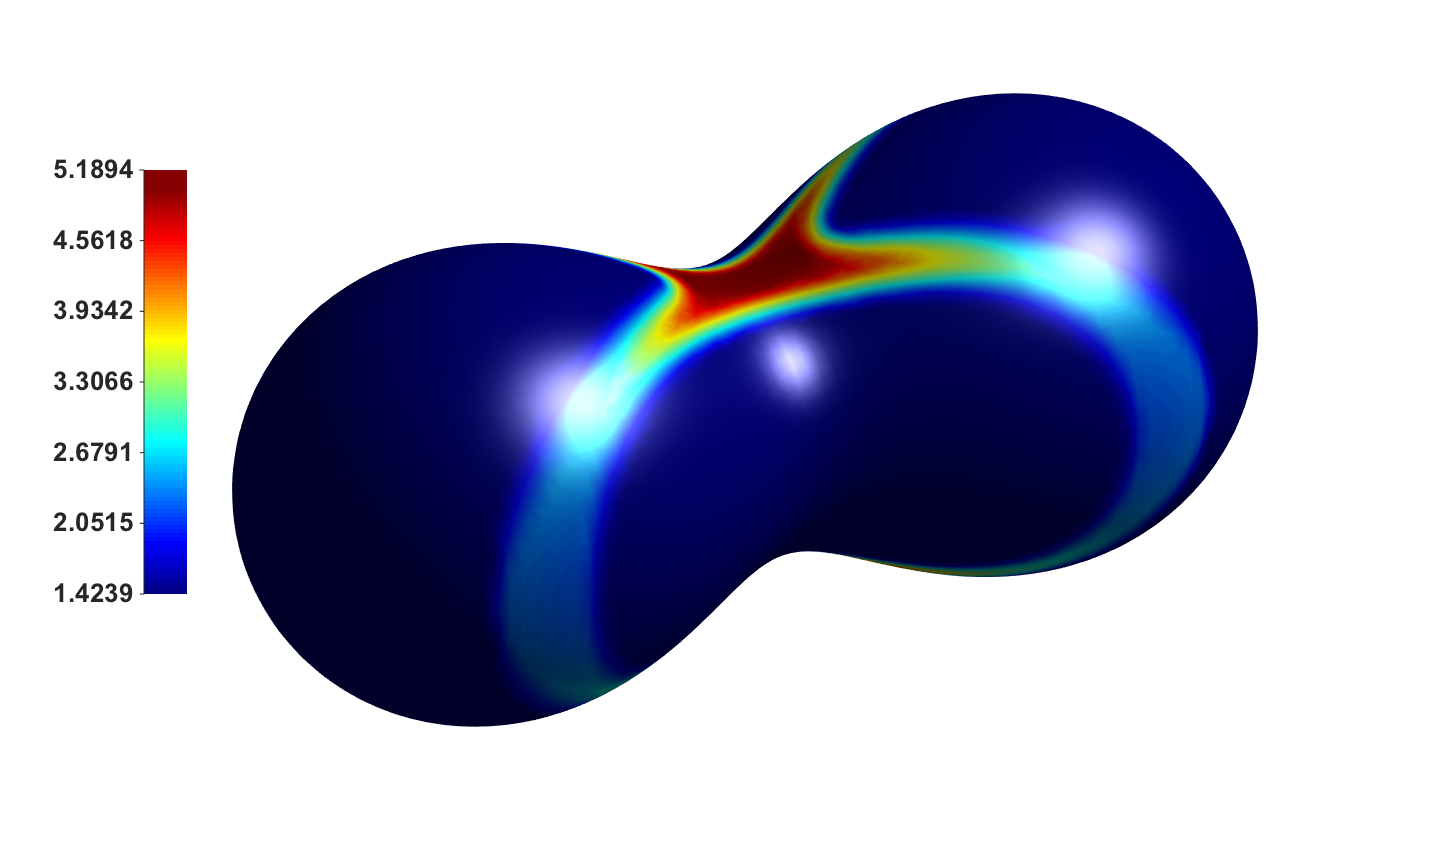
\includegraphics[width=10cm]{../figures/Molecular_Solution.png} & \quad & 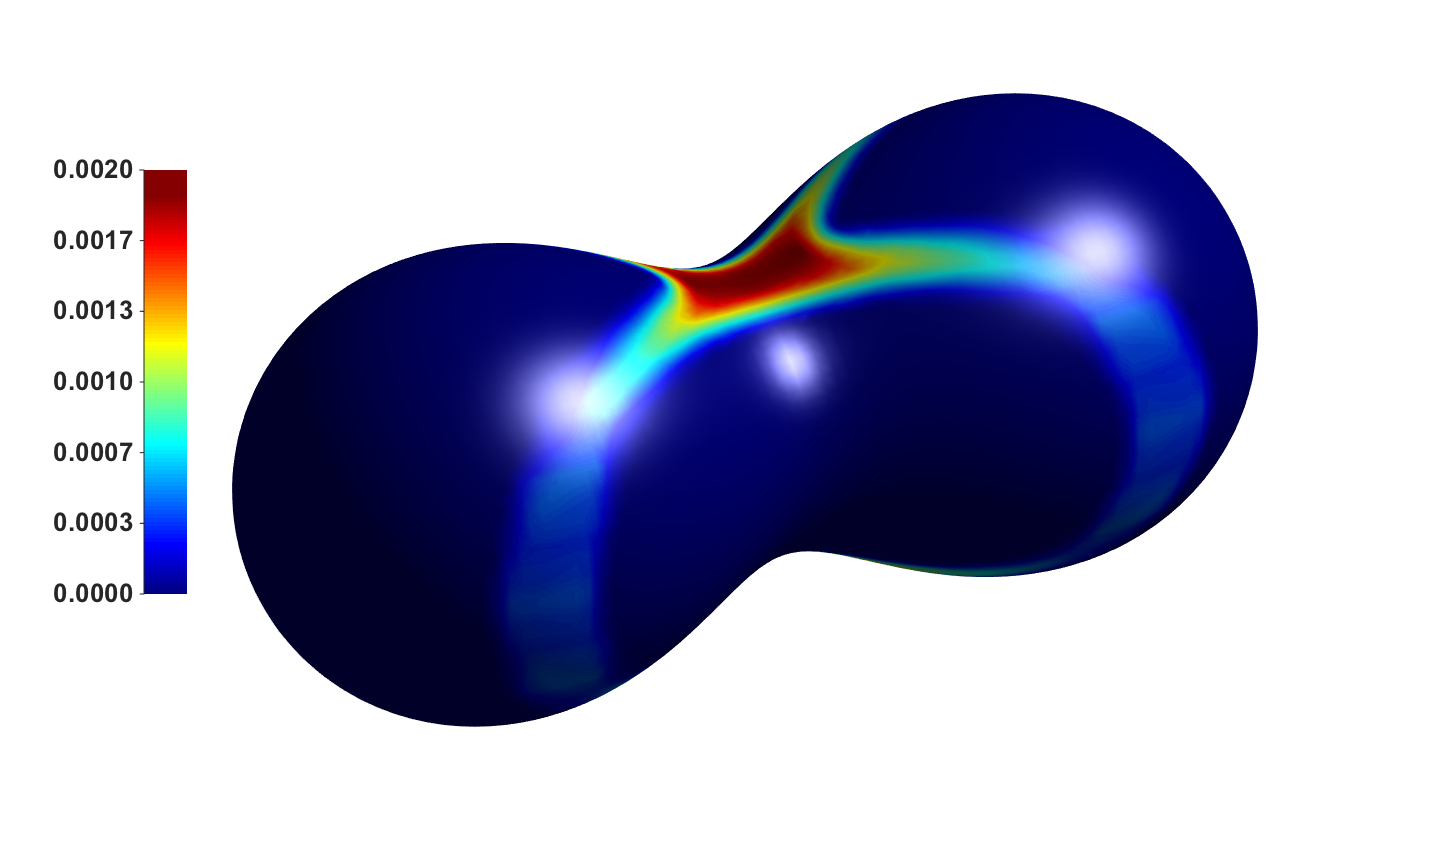
\includegraphics[width=10cm]{../figures/Molecular_Error.png} \\ 
				\textbf{(a)} & \quad & \textbf{(b)}
		\end{tabular}}
	\end{center}
	\caption{Color maps for molecular surface. (a). numerical solution; (b). numerical error.}
	\label{fig:color_map_molecular}
\end{figure*}
%
The concave region which connects the two atoms makes it impossible to derive the jump conditions $[\alpha u_{\eta}]$ and $[\alpha u_{\zeta}]$ without approximating the tangential derivative $u_{\eta}$ and $u_{\zeta}$ in both outer and inner domains ($\Omega^{+}$ and $\Omega^{-}$) simultaneously. The same analytical solution \eqref{analytical_eqn_1} and source term \eqref{source_eqn_1} with $a=1$ are used. 


%
%\noindent
\begin{table}
	\centering
	\renewcommand{\arraystretch}{1.0}% Tighter
	\resizebox{\textwidth}{!}{
		\tiny
		\begin{tabular}{c @{\hskip 8mm} cccccccc @{}}\midrule
			\multirow{2}{*}{$[N_{x},N_{y},N_{z}]$} 
			%&\multicolumn{5}{c}{Example 3} \\ 
			%\cmidrule{2-6}
			&\multicolumn{2}{c}{$L_{\infty}$}  & \phantom{abc} &\multicolumn{2}{c}{$L_2$} \\ 
			\cmidrule{2-3} \cmidrule{5-6}
			&\multicolumn{1}{c}{Error}  &\multicolumn{1}{c}{Order}  & \phantom{abc} 
			&\multicolumn{1}{c}{Error}  &\multicolumn{1}{c}{Order} \\
			\hline
			$[20,20,20]$      & 2.135e-01  &        & & 2.140e-02  &      \\
			$[40,40,40]$      & 4.341e-02  & 2.30   & & 3.833e-03  & 2.48 \\
			$[80,80,80]$      & 1.128e-02  & 1.94   & & 1.143e-03  & 1.75 \\
			$[160,160,160]$   & 2.645e-03  & 2.09   & & 2.503e-04  & 2.19 \\
			\hline
	\end{tabular}}
	\captionof{table}{Spatial convergence for molecular surface.}
	\label{table:molecule}
\end{table}
%
%
\begin{figure*}[!tb] 
	\centering
	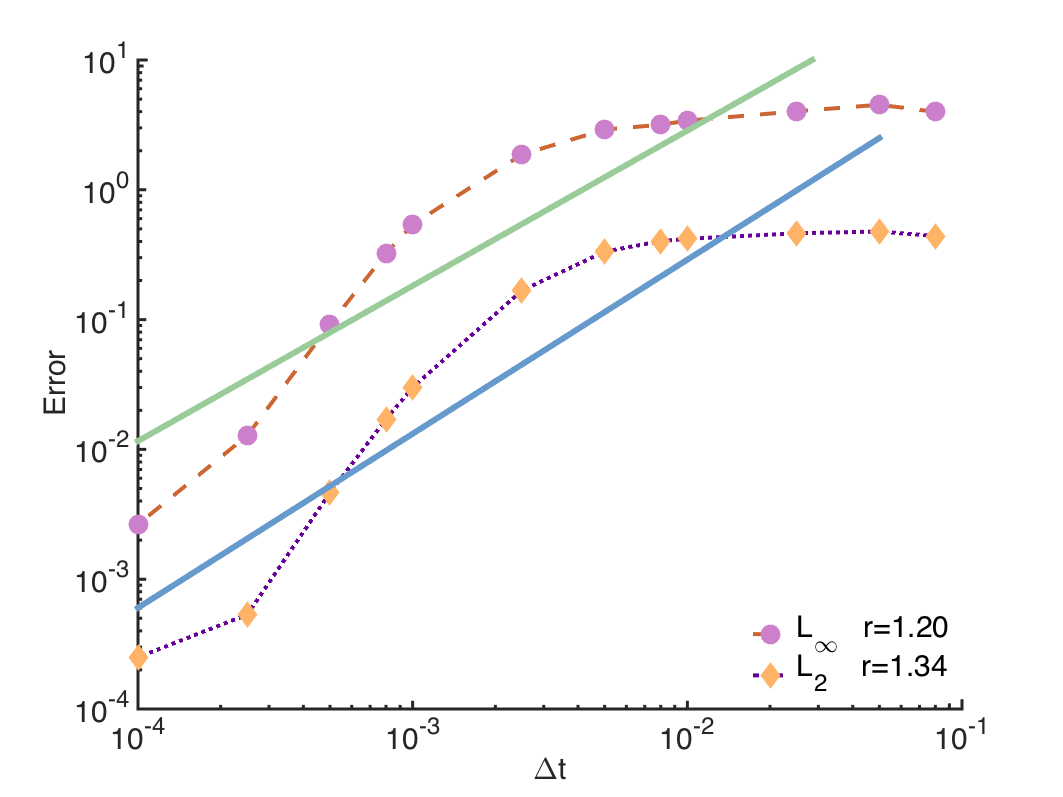
\includegraphics[width=12cm]{../figures/Molecular_Time.png}
	\captionof{figure}{Temporal convergence for molecular surface.}
	\label{fig:temporal_convergence_molecule}
\end{figure*}
%
\begin{figure}[!ht] 
	\begin{center}
		\resizebox{\textwidth}{!}{
			\begin{tabular}{ccc}
				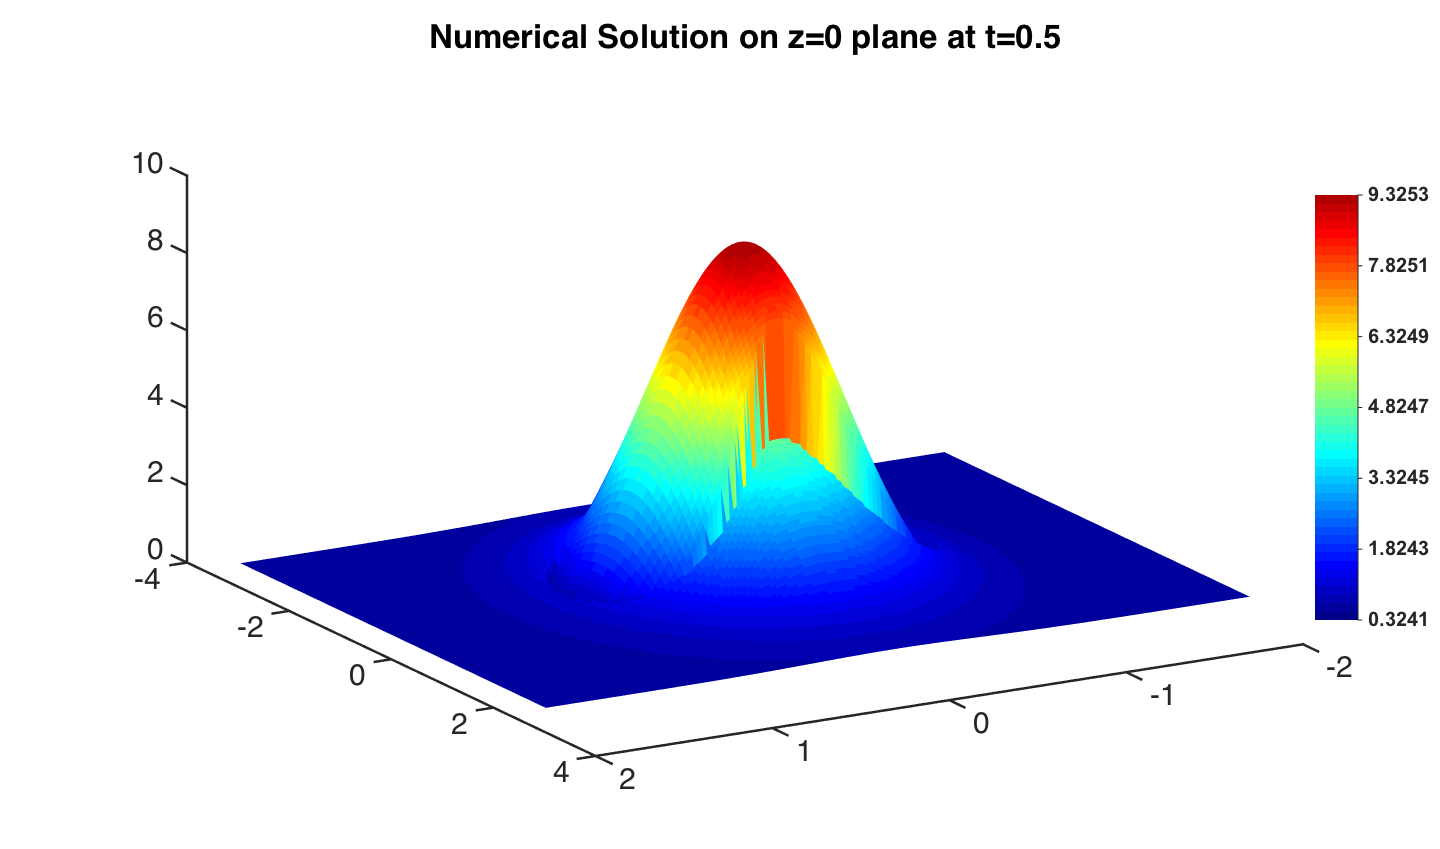
\includegraphics[width=15cm]{../figures/Molecular_1.png} & \quad & 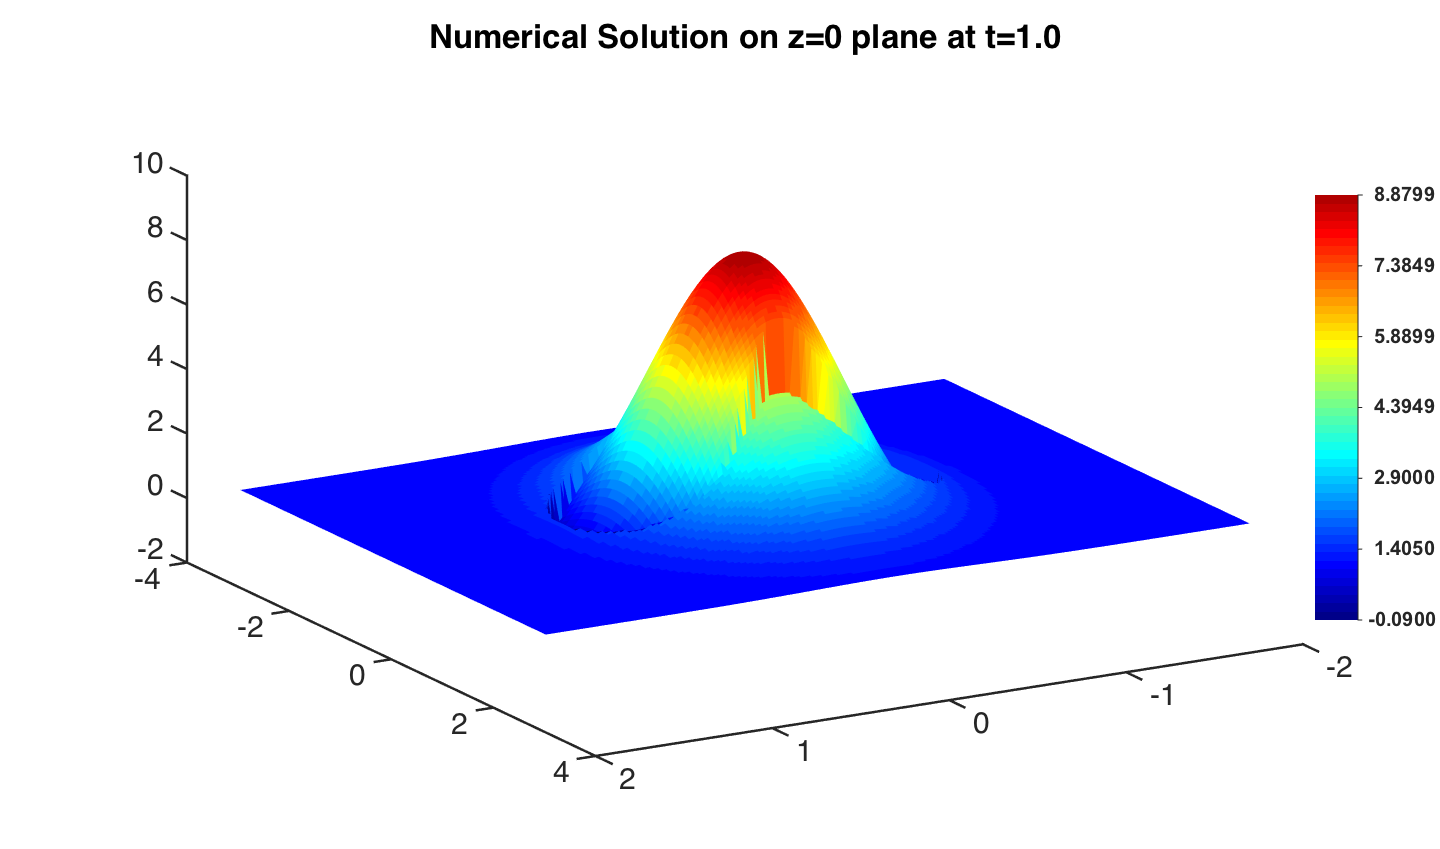
\includegraphics[width=15cm]{../figures/Molecular_2.png} \\ 
				\textbf{(a)} & \quad & \textbf{(b)} \\
				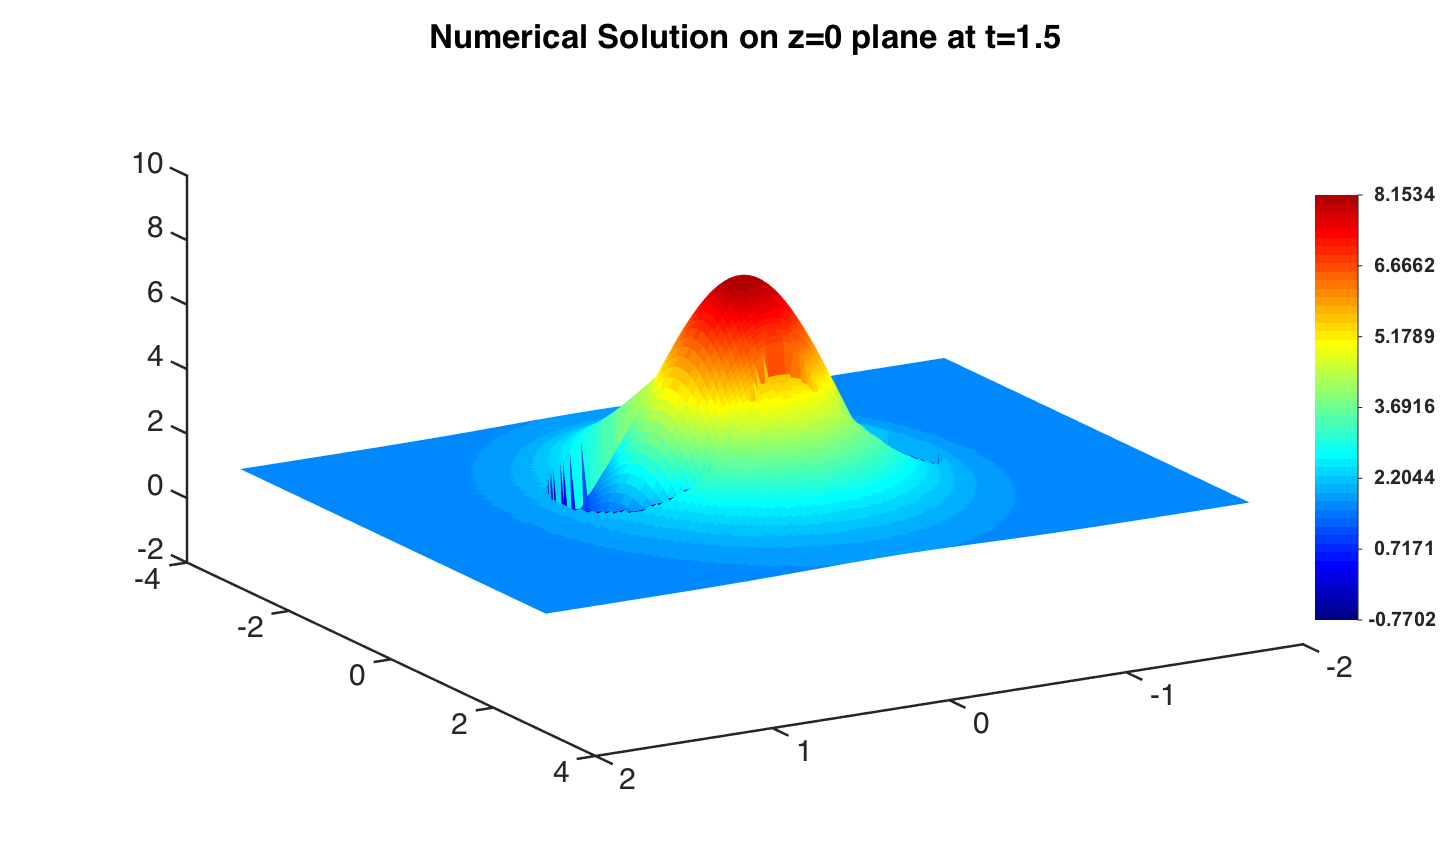
\includegraphics[width=15cm]{../figures/Molecular_3.png} & \quad & 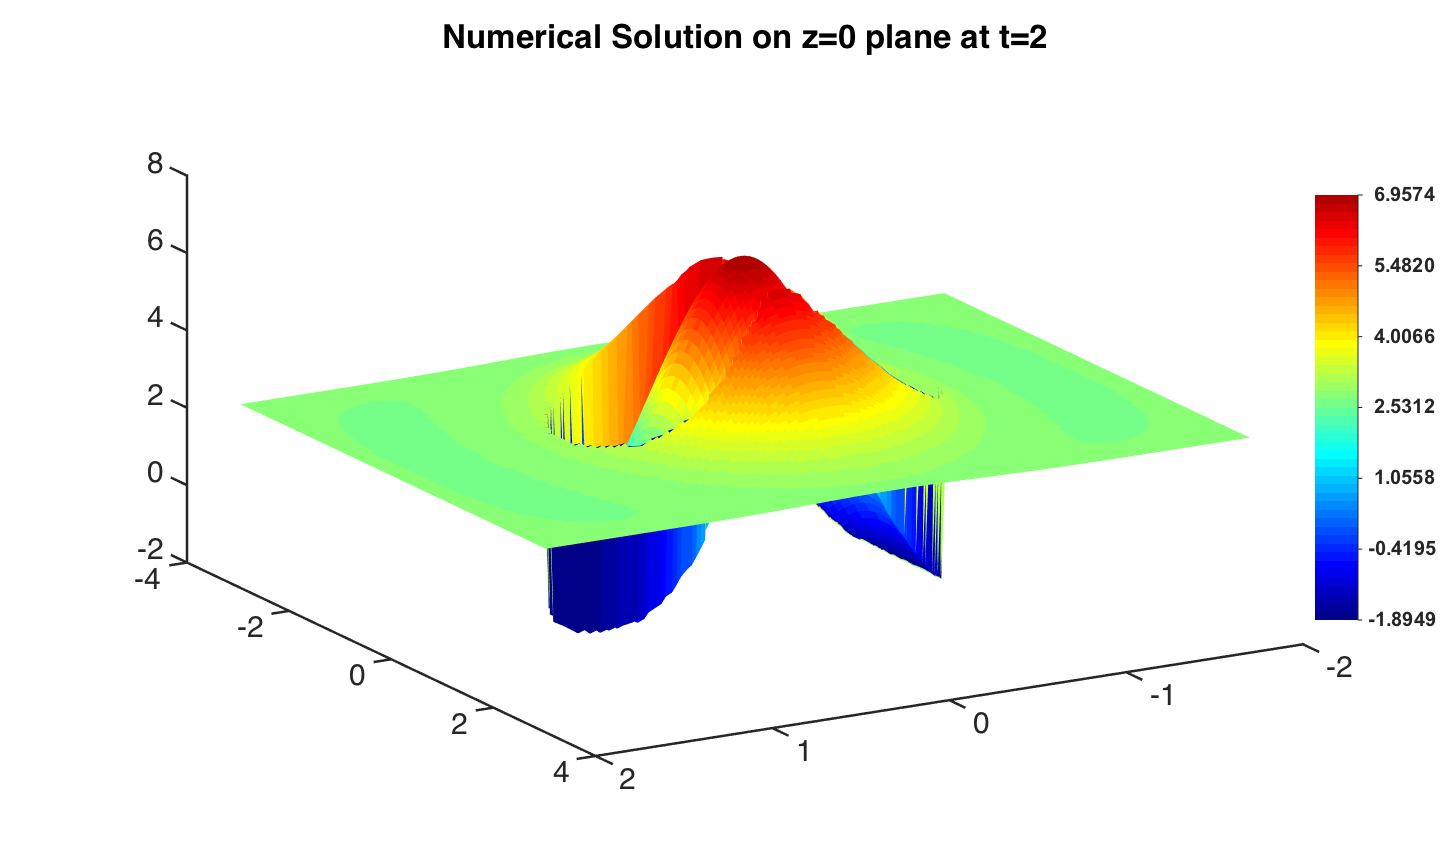
\includegraphics[width=15cm]{../figures/Molecular_4.png} \\ 
				\textbf{(c)} & \quad & \textbf{(d)}
		\end{tabular}}
	\end{center}
	\caption{Slice plots of the numerical solutions on $z=0$ plane in Example 3. 
		(a) $t=0.5$; (b) $t=1$; (c) $t=1.5$; (d) $t=2$. }
	\label{fig:molecular_mesh}
\end{figure}

\begin{figure}[!ht] 
	\begin{center}
		\resizebox{\textwidth}{!}{
			\begin{tabular}{ccc}
				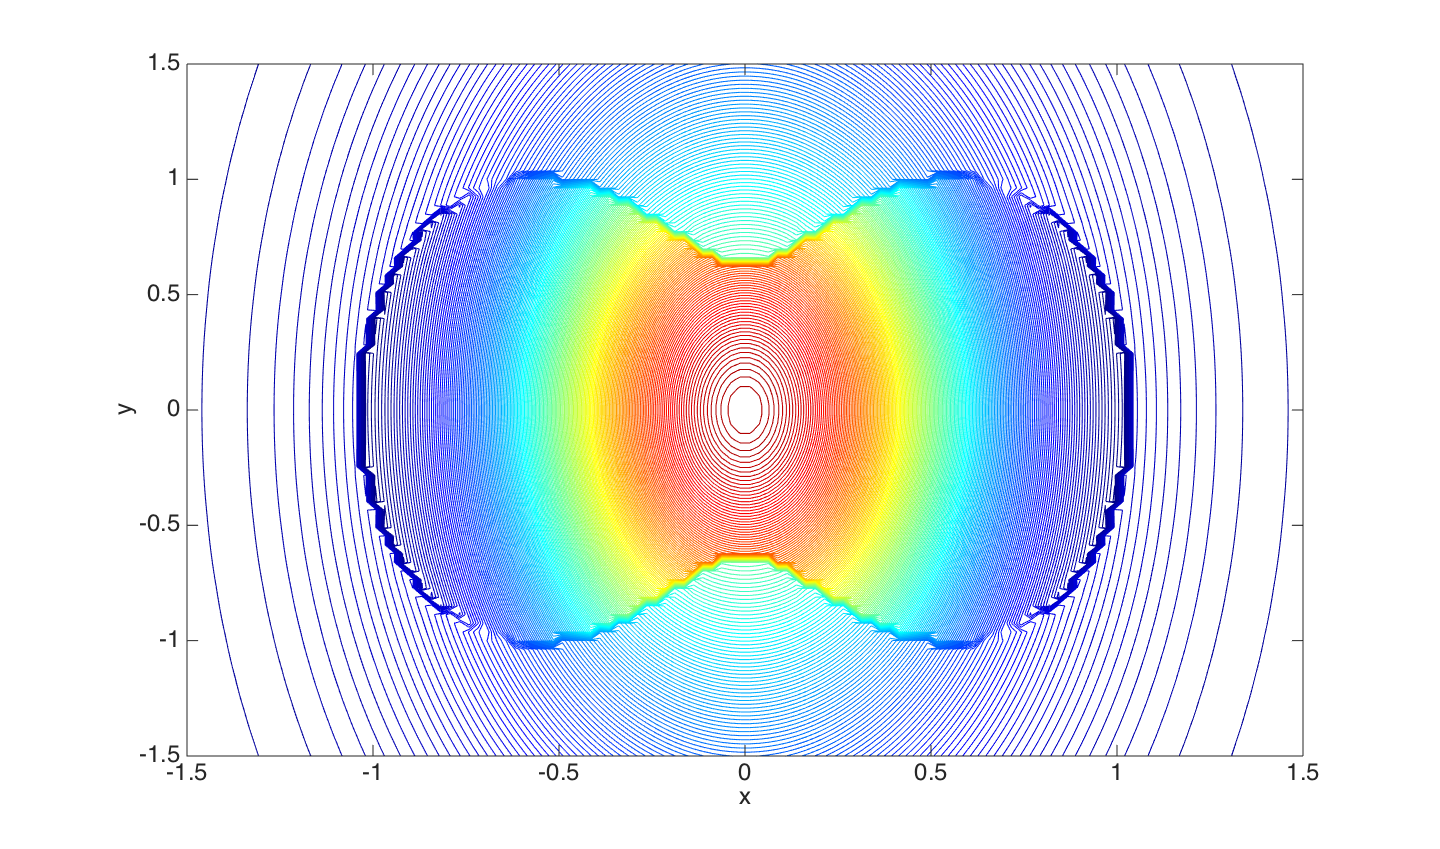
\includegraphics[width=15cm]{../figures/Molecular_Contour_1.png} & \quad & 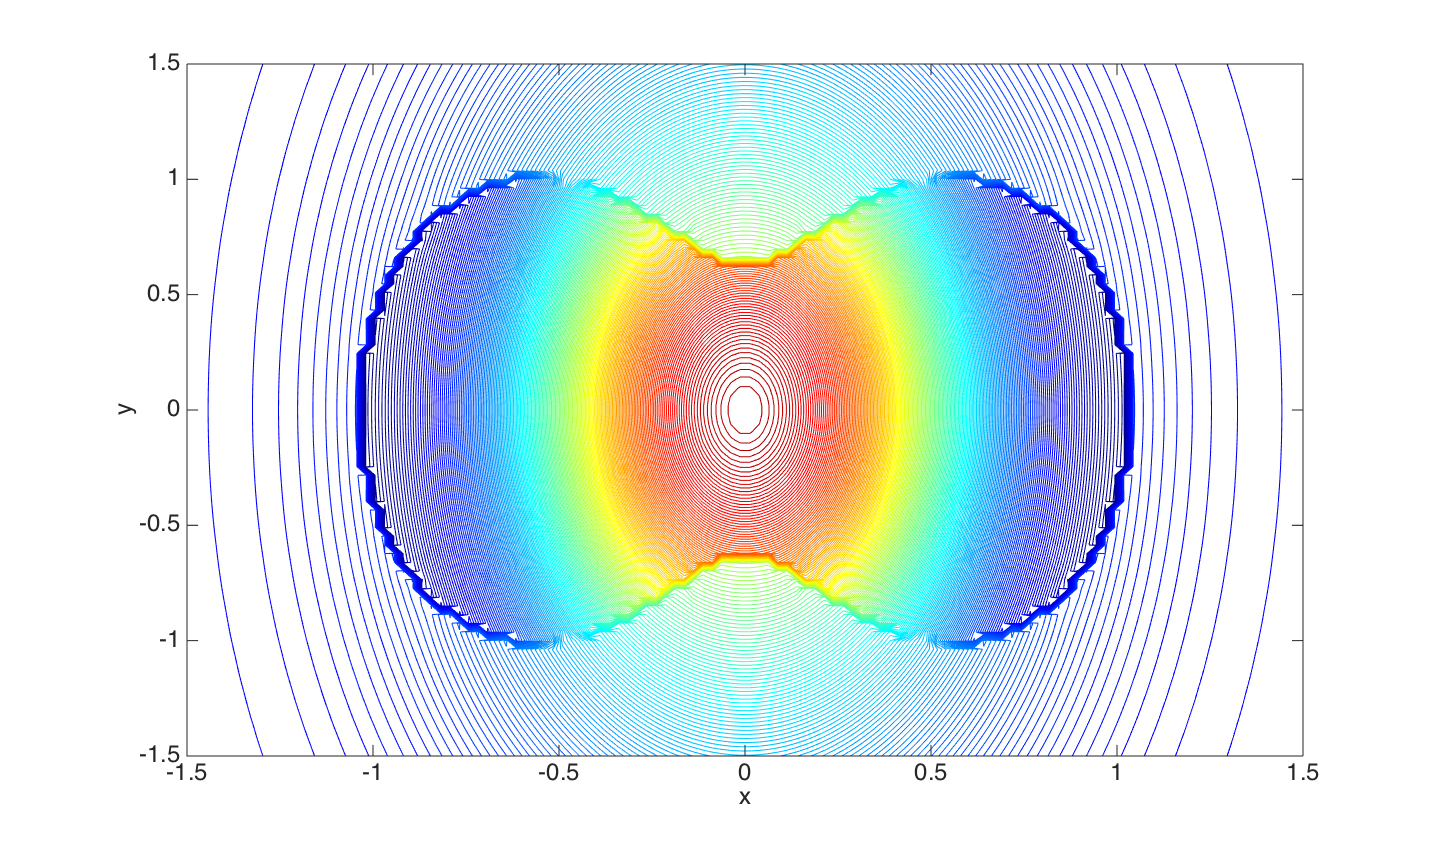
\includegraphics[width=15cm]{../figures/Molecular_Contour_2.png} \\ 
				\textbf{(a)} & \quad & \textbf{(b)} \\
				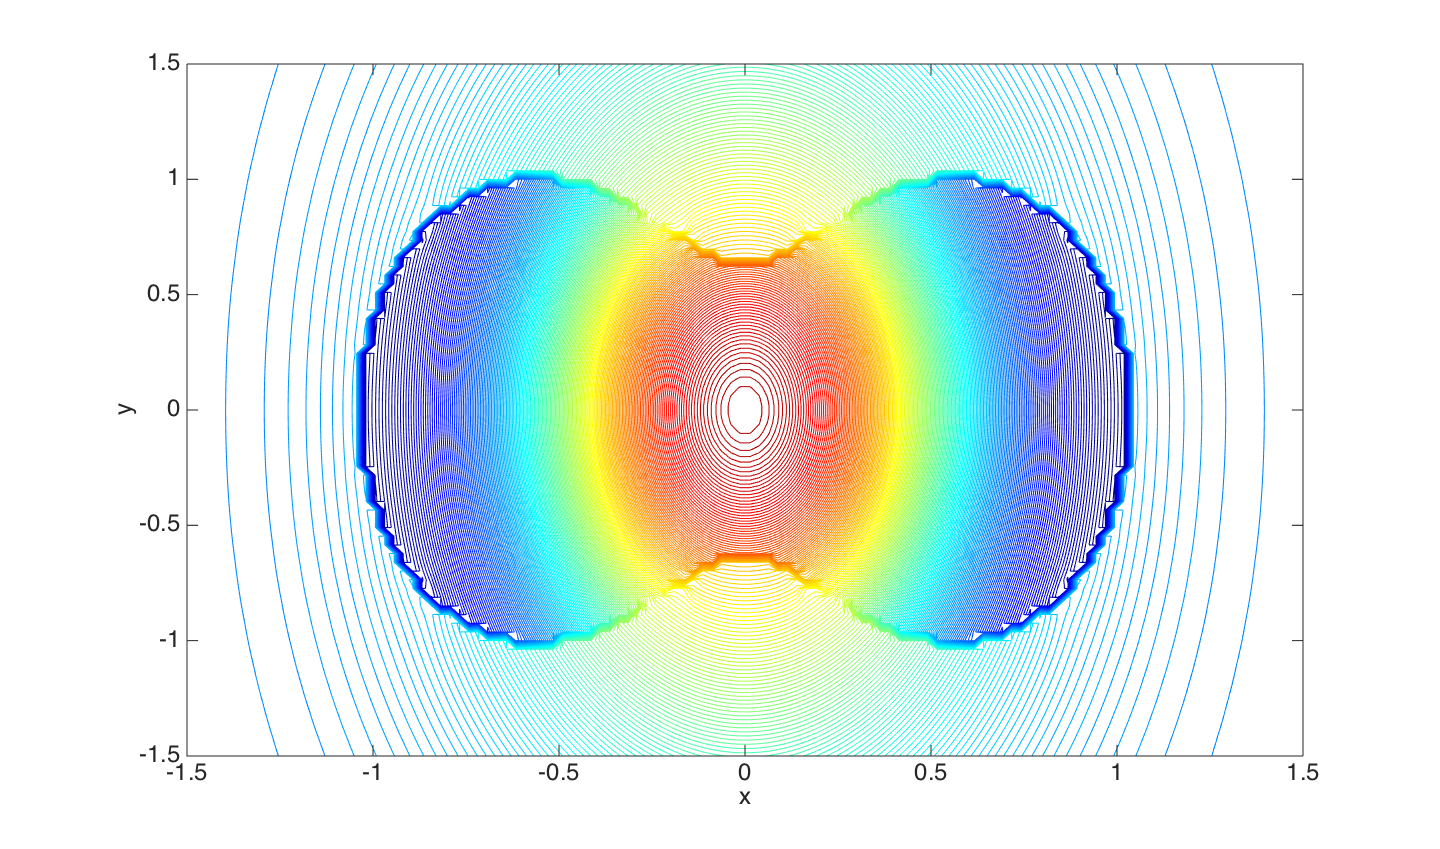
\includegraphics[width=15cm]{../figures/Molecular_Contour_3.png} & \quad & 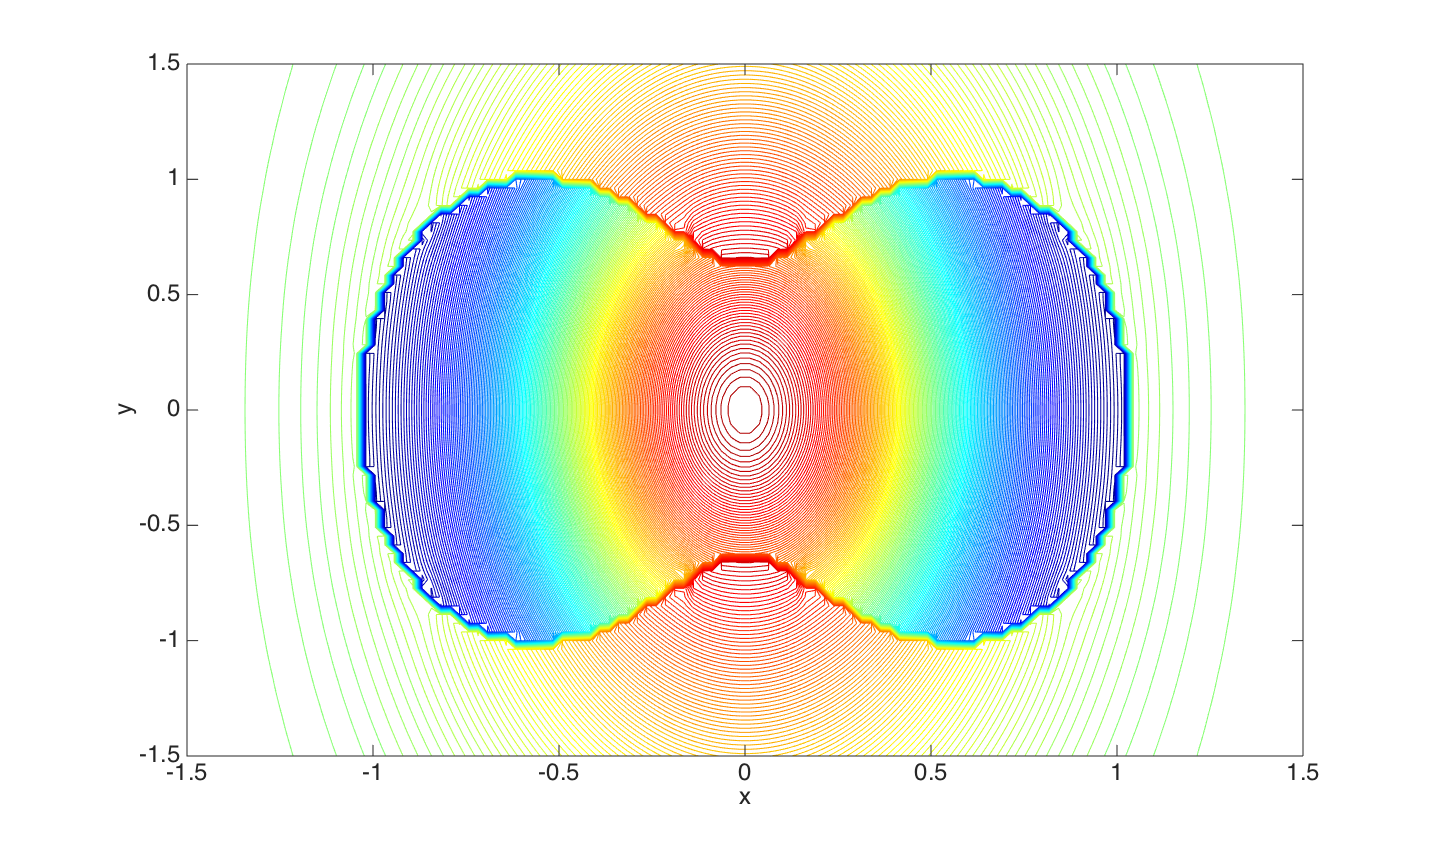
\includegraphics[width=15cm]{../figures/Molecular_Contour_4.png} \\ 
				\textbf{(c)} & \quad & \textbf{(d)}
		\end{tabular}}
	\end{center}
	\caption{Contour plots of the numerical solutions on $z=0$ plane in Example 3.
		(a) $t=0.5$; (b) $t=1$; (c) $t=1.5$; (d) $t=2$. }
	\label{fig:molecular_contour}
\end{figure}
%


Once again, the proposed matched ADI method is stable and converges for all tested $h$ and $\Delta t$. To demonstrate the results, $\Delta t=10^{-4}$ is fixed for spatial convergence tests and the results are shown in Table \ref{table:molecule}. The results clearly conclude that the spatial convergence rate is two. The results obtained for the temporal convergence test by fixing the number of grids per direction to be 160 are shown in Figure  \ref{fig:temporal_convergence_molecule}, together with the results of lease-squares error analysis. In this case, both $L_{\infty}$ and $L_2$ errors decrease in a similar manner. Although it is not very uniform for all $\Delta t$'s, the overall order of the matched ADI method is still higher than one for both error measurements.
The color map of numerical solutions and errors are illustrated in Figure \ref{fig:color_map_molecular} for  $[N_{x},N_{y},N_{z}]=[160,160,160]$ and $\Delta t=10^{-4}$. The error distribution pattern is almost the same as that of the solution. 

To appreciate the numerical difficulty of the present parabolic interface problem, the slice plots of the 
matched ADI solutions at the cross section $z=0$ are depicted in Fig. \ref{fig:molecular_mesh}.
Here, we take $[N_{x},N_{y},N_{z}]=[160,160,160]$ and carry out the integration from $t=0$ to $t=2$ with
$\Delta t=10^{-3}$. 
As shown in Fig. \ref{fig:molecular_mesh}, a strong jump discontinuity is developed in the solution as time increases. 
To view the hidden solution in the other side, the corresponding contour plots are shown in 
Fig. \ref{fig:molecular_contour}.
Without plotting the interface $\Gamma$ explicitly, these contour lines clearly show the location
of $\Gamma$. Even though the solution pattern inside $\Gamma$ is unchanged, the contrast of the solutions
inside and outside $\Gamma$ is variant. A strong jump discontinuity can also be sensed in the contour
plot at time $t=2$, because the contour lines now undergo a fast and sharp change near the interface. 

%----------------------------------------------------------------------%
%                                                                      %
%                               Example 4                              %
%                                                                      %
%----------------------------------------------------------------------%

{\flushleft \bf Example 4.} This example examines the performance of the proposed method on fully time-dependent jump conditions. To this end, we consider a smooth torus, which is given as the zero level set of
%
\begin{equation}
S(x,y,z) = (\frac{3}{2}-\sqrt{x^{2}+y^{2}})^{2}+z^{2}-\frac{49}{100}
\end{equation}
%
in a computational domain of dimension $[-3.99,3.99]\times[-3.99,3.99]\times[-3.99,3.99]$. The analytical solution is constructed in the form of 
%
\begin{equation} \label{analytical_eqn_2}
u(x,y,z,t)= 
\begin{cases}
\cos(ax)\sin(ay)\cos(az)\cos(t)-1, \quad   &\mbox{in } \Omega^{-} \\
\sin(ax)\cos(ay)\sin(az)\cos(t)+1,  \quad   &\mbox{in } \Omega^{+}
\end{cases}
\end{equation}
%
so that $a=2$ yields a periodic solution with a period of $\pi$. The source term is given by
%
\begin{equation} \label{source_eqn_2}
f(x,y,z,t)= 
\begin{cases}
(3 \alpha^{-} a^{2}\cos(t)-\sin(t)) \cos(ax)\sin(ay)\cos(az) \quad   &\mbox{in } \Omega^{-} \\
(3 \alpha^{+} a^{2}\cos(t)-\sin(t)) \sin(ax)\cos(ay)\sin(az)  \quad   &\mbox{in } \Omega^{+}.
\end{cases}
\end{equation}
%
In this example, the interface jump conditions are time-and-space dependent, which represents the most general physical jump conditions for parabolic interface problems. 

%\noindent
\begin{table}
	\centering
	\renewcommand{\arraystretch}{1.0}% Tighter
	\resizebox{\textwidth}{!}{
		\tiny
		\begin{tabular}{c @{\hskip 8mm} cccccccc @{}}\midrule
			\multirow{2}{*}{$[N_{x},N_{y},N_{z}]$} 
			%&\multicolumn{5}{c}{Example 4} \\ 
			%\cmidrule{2-6}
			&\multicolumn{2}{c}{$L_{\infty}$}  & \phantom{abc} &\multicolumn{2}{c}{$L_2$} \\ 
			\cmidrule{2-3} \cmidrule{5-6}
			&\multicolumn{1}{c}{Error}  &\multicolumn{1}{c}{Order}  & \phantom{abc} 
			&\multicolumn{1}{c}{Error}  &\multicolumn{1}{c}{Order} \\
			\hline
			$[20,20,20]$      & 2.774e-01  &        & & 1.908e-02  &      \\
			$[40,40,40]$      & 3.803e-02  & 2.87   & & 2.767e-03  & 2.79 \\
			$[80,80,80]$      & 1.146e-02  & 1.73   & & 6.554e-04  & 2.08 \\
			$[160,160,160]$   & 8.254e-03  & 0.47   & & 1.602e-04  & 2.03 \\
			\hline
	\end{tabular}}
	\captionof{table}{Spatial convergence for torus surface.}
	\label{table:torus}
\end{table}
%
%
\begin{figure*}[!tb] 
	\centering
	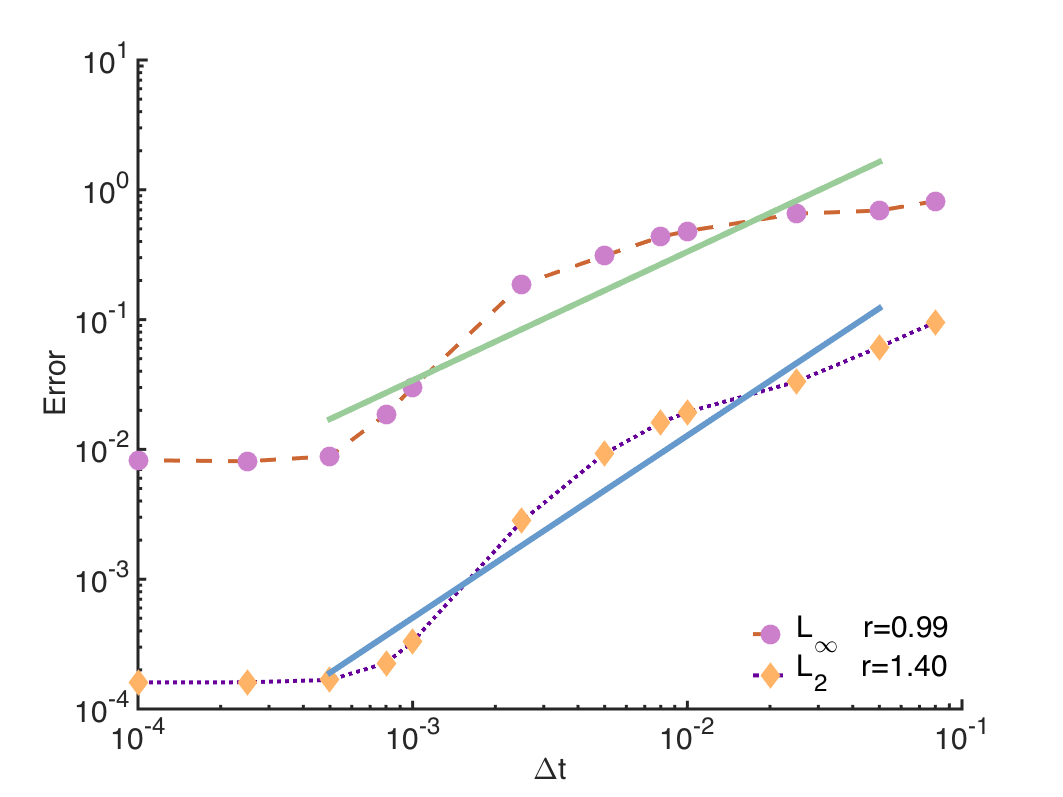
\includegraphics[width=12cm]{../figures/Torus_Time.png}
	\captionof{figure}{Temporal convergence for torus surface.}
	\label{fig:temporal_convergence_torus}
\end{figure*}
%

The 3D matched ADI method is stable for this example, and 
the results obtained by the spatial convergence tests are presented in Table \ref{table:torus}. It can be observed that the convergence rate in the $L_2$ norm is still two. However, the $L_{\infty}$ convergence becomes a little deteriorated in this example, especially for the last entry, even though the overall rate is still about $1.6$. 
The temporal tests are shown in Figure \ref{fig:temporal_convergence_torus} which reveals a similar pattern,  i.e., the $L_2$ order is similar to the previous examples, while the $L_{\infty}$ rate is affected somehow. 
For more detailed insights, the color maps are demonstrated in Figure \ref{fig:color_map_torus}. We can see that the error distribution pattern is quite random in this example, which means that  some large errors occur on or near the interface $\Gamma$, even when the solution or its gradient is not large. The $L_{\infty}$ convergence patterns shall be related to such an irregular error distribution. 

%
\begin{figure*}[!ht]
	\begin{center}
		\resizebox{\textwidth}{!}{
			\begin{tabular}{ccc}
				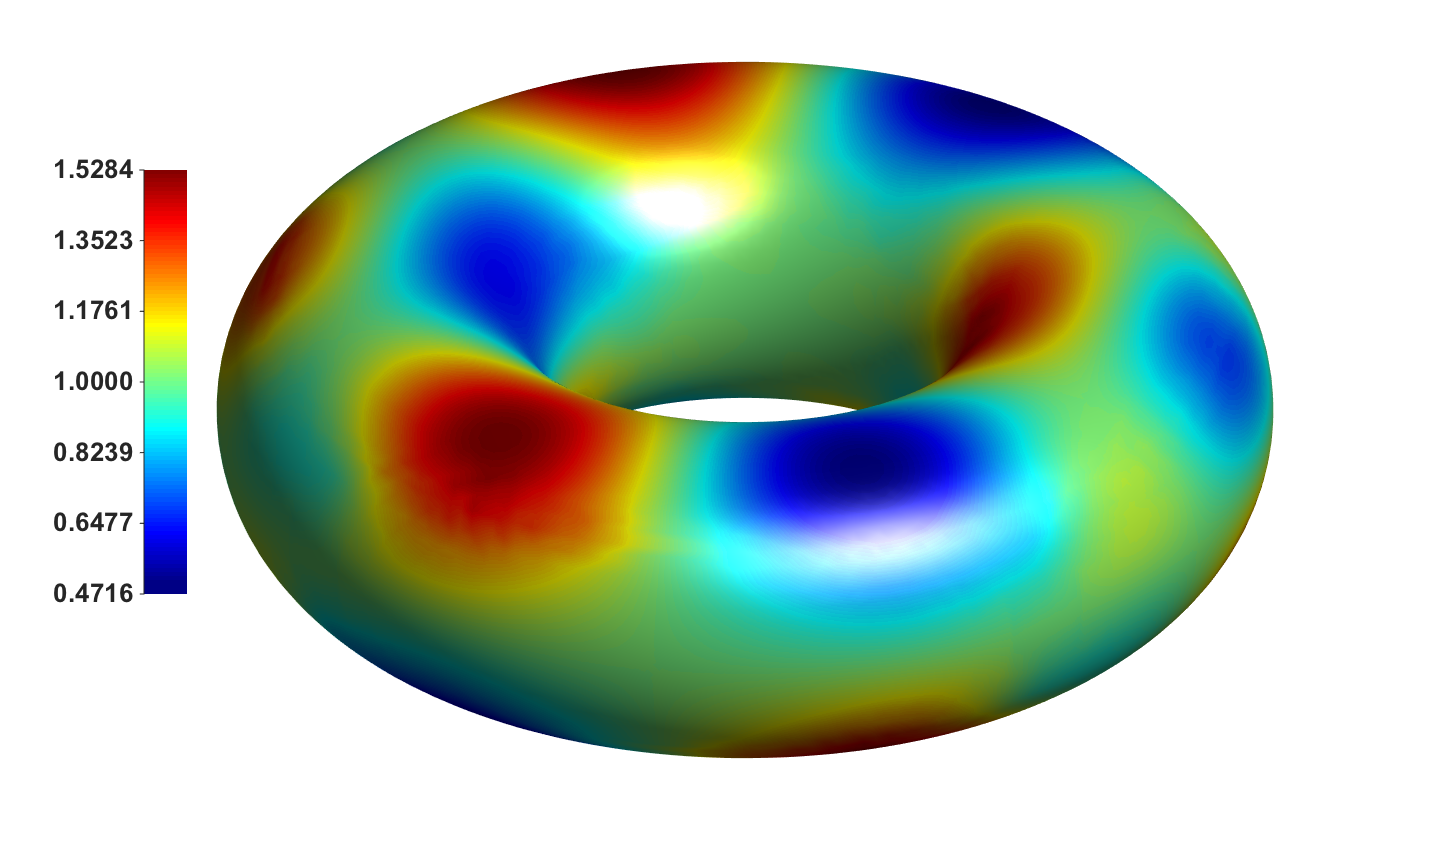
\includegraphics[width=10cm]{../figures/Torus_Solution.png} & \quad & 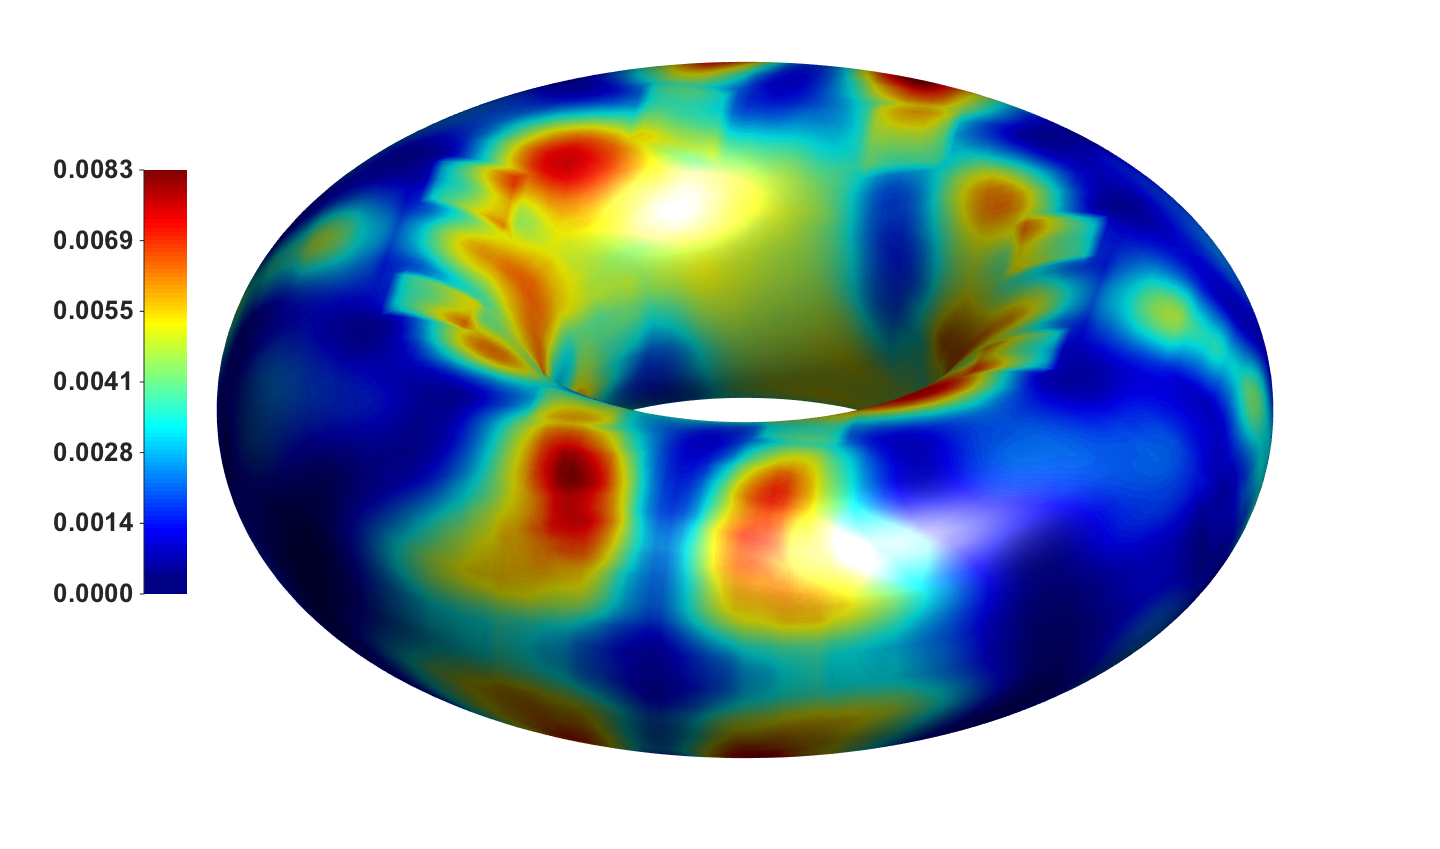
\includegraphics[width=10cm]{../figures/Torus_Error.png} \\ 
				\textbf{(a)} & \quad & \textbf{(b)}
		\end{tabular}}
	\end{center}
	\caption{Color maps for torus surface. (a). numerical solution;
		(b). numerical error.}
	\label{fig:color_map_torus}
\end{figure*}

%----------------------------------------------------------------------%
%                                                                      %
%                               Example 5                              %
%                                                                      %
%----------------------------------------------------------------------%


{\flushleft \bf Example 5.} This example deals with a complicated topological shape of a tanglecube, defined as the zero level set of 
%
\begin{equation} \label{tanglecube}
S(x,y,z) = x^{4}-5x^{2}+y^{4}-5y^{2}+z^{4}-5z^{2}+10. 
\end{equation}
%
embedded in a domain of dimension $[-3.99,3.99]\times[-3.99,3.99]\times[-4.99,4.99]$. The tanglecube surface has several convex and concave regions which pose grant challenges for the tangential derivative approximations. The previous analytical solution \eqref{analytical_eqn_2} is reused with a different coefficient $a=1$ so that all jump conditions are still time dependent. For this example, one grid line will cut the interface in zero, two or four times. 

The matched ADI method is stable for this example. 
Similar spatial and temporal tests are repeated and the results are shown in Table \ref{table:tanglecube} and Figure \ref{fig:temporal_convergence_tanglecube}, respectively, together with the color maps shown in Figure \ref{fig:color_map_tanglecube}. 
Even though the convergence is not uniform, the averaged spatial convergence rates in both error norms are above two. The temporal convergence rate is similar to what obtained in previous examples. 
Moreover, the color maps show that the maximum errors occur not only in the regions where the solution achieves maximum values, but also in the regions where the largest jumps take place across the interface.

%\noindent
\begin{table}
	\centering
	\renewcommand{\arraystretch}{1.0}% Tighter
	\resizebox{\textwidth}{!}{
		\tiny
		\begin{tabular}{c @{\hskip 8mm} cccccccc @{}}\midrule
			\multirow{2}{*}{$[N_{x},N_{y},N_{z}]$} 
			%&\multicolumn{5}{c}{Example 5} \\ 
			%\cmidrule{2-6}
			&\multicolumn{2}{c}{$L_{\infty}$}  & \phantom{abc} &\multicolumn{2}{c}{$L_2$} \\ 
			\cmidrule{2-3} \cmidrule{5-6}
			&\multicolumn{1}{c}{Error}  &\multicolumn{1}{c}{Order}  & \phantom{abc} 
			&\multicolumn{1}{c}{Error}  &\multicolumn{1}{c}{Order} \\
			\hline
			$[20,20,20]$      & 2.394e-01  &        & & 1.743e-02  &      \\
			$[40,40,40]$      & 6.940e-02  & 1.79   & & 4.890e-03  & 1.83 \\
			$[80,80,80]$      & 2.162e-03  & 5.00   & & 2.688e-04  & 4.19 \\
			$[160,160,160]$   & 1.112e-03  & 0.96   & & 7.762e-05  & 1.79 \\
			\hline
	\end{tabular}}
	\captionof{table}{Spatial convergence for tanglecube surface.}
	\label{table:tanglecube}
\end{table}
%
%
\begin{figure*}[!tb] 
	\centering
	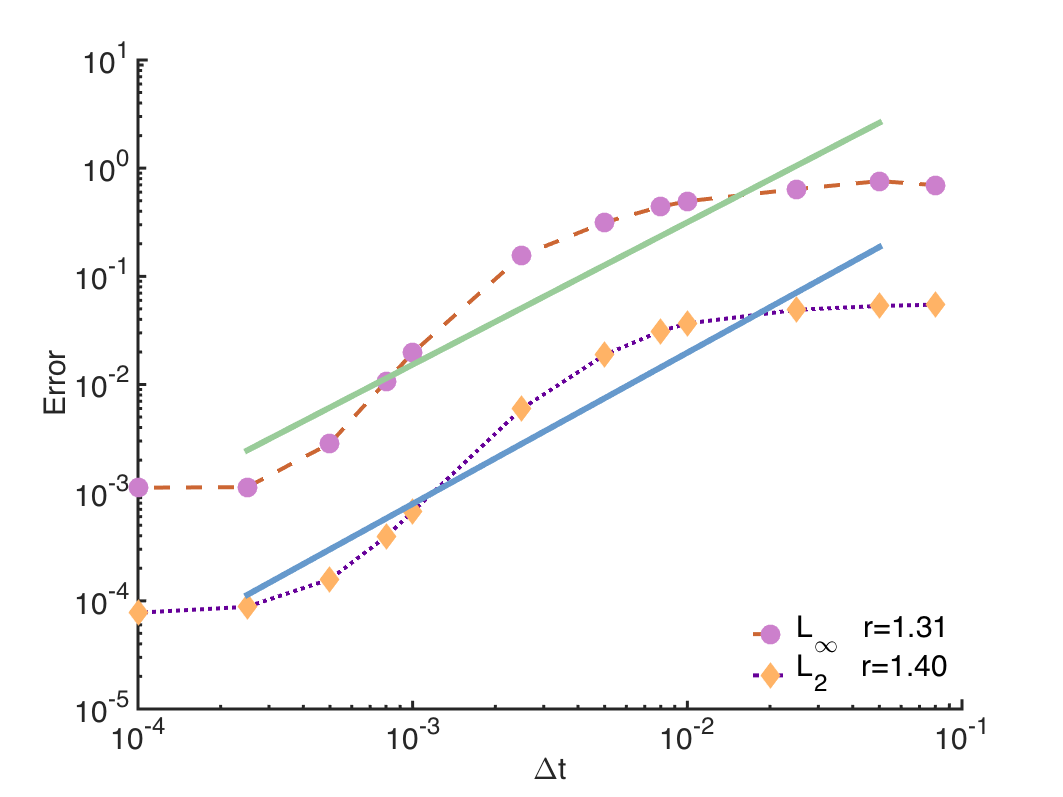
\includegraphics[width=12cm]{../figures/Tanglecube_Time.png}
	\captionof{figure}{Temporal convergence for tanglecube surface.}
	\label{fig:temporal_convergence_tanglecube}
\end{figure*}
%
\begin{figure*}[!hb]	
	\begin{center}
		\resizebox{\textwidth}{!}{
			\begin{tabular}{ccc}
				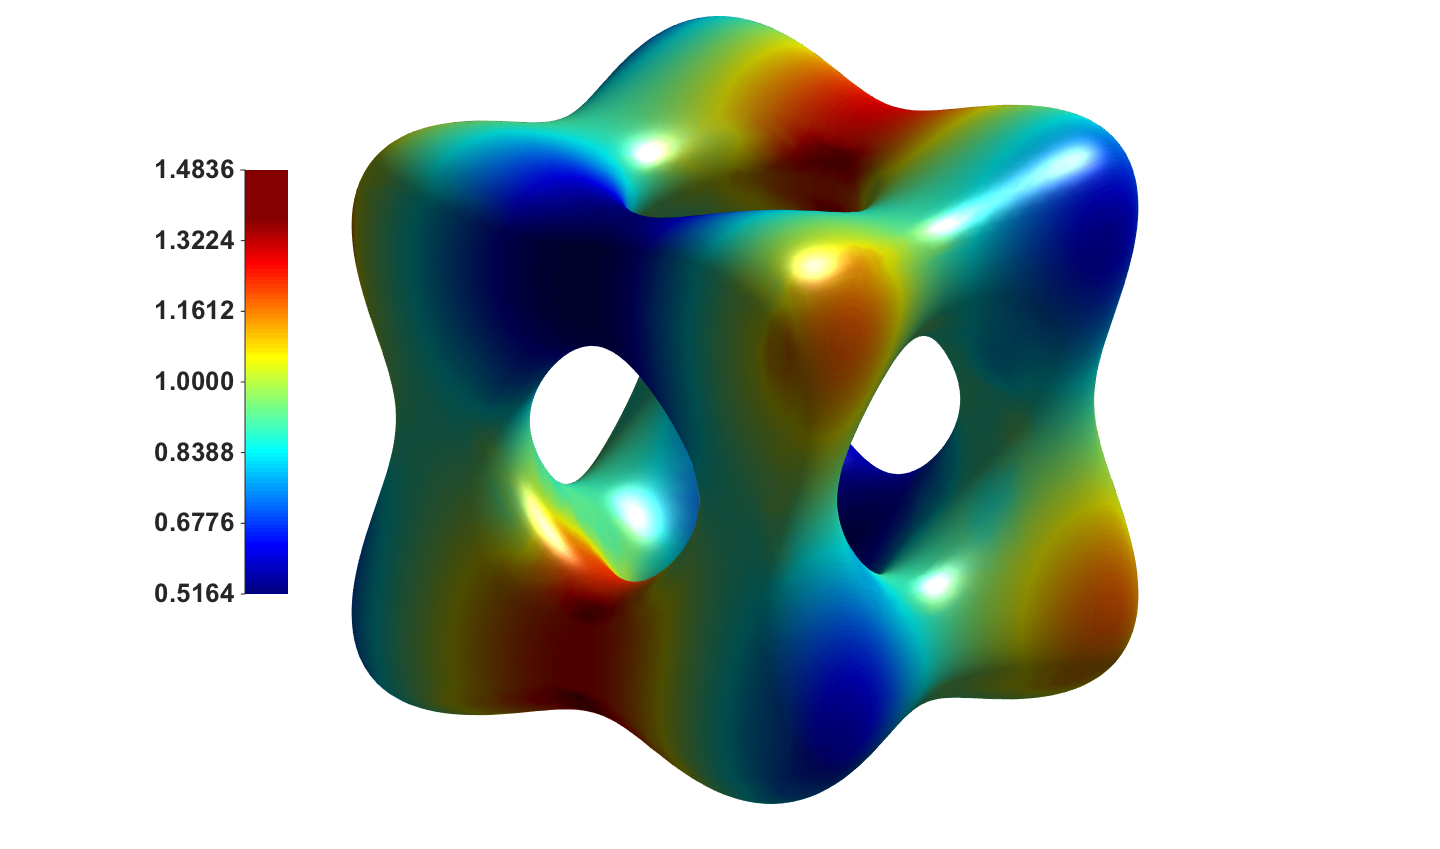
\includegraphics[width=10cm]{../figures/Tanglecube_Solution.png} & \quad & 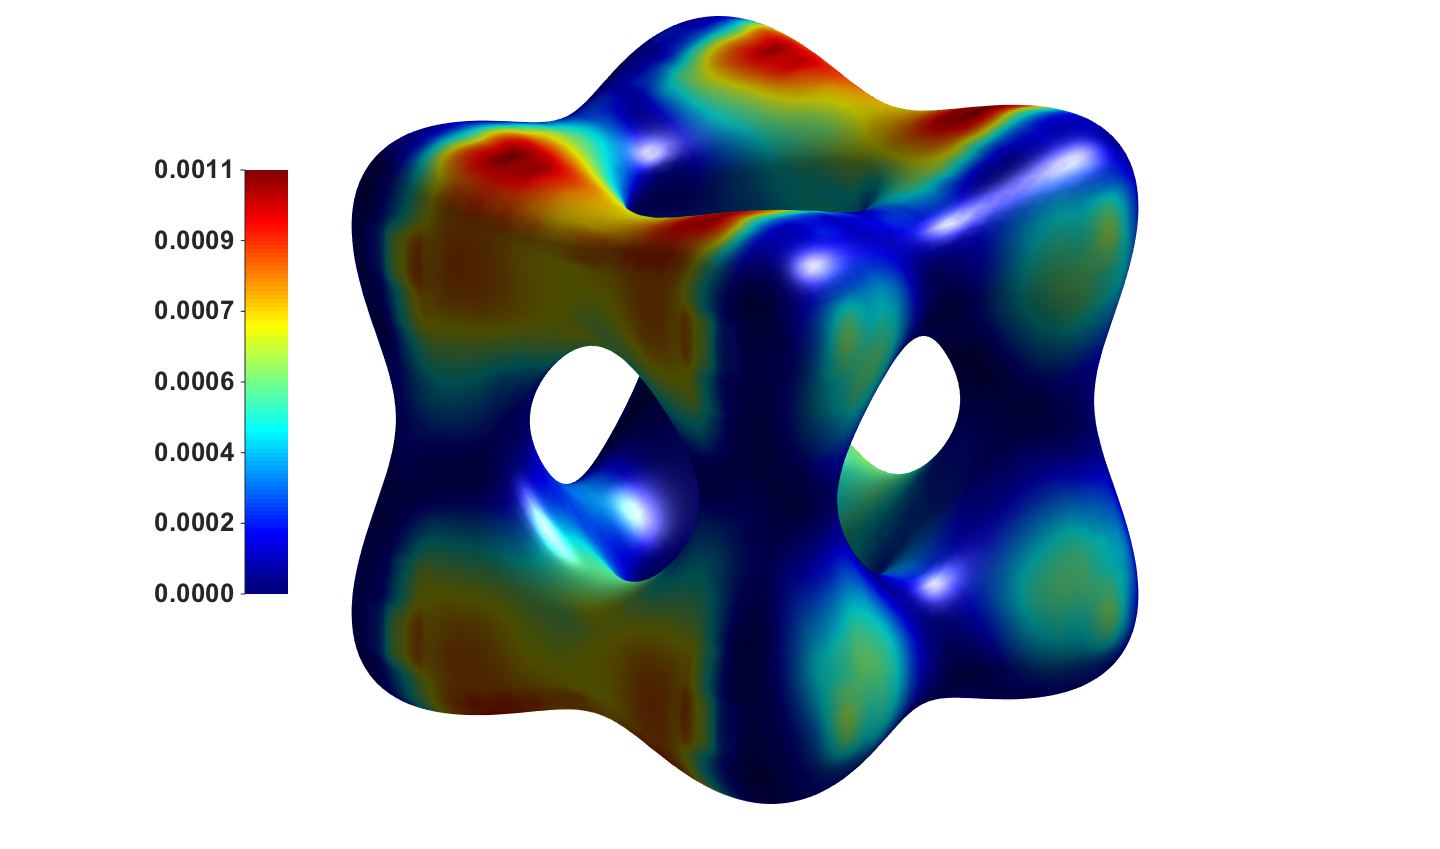
\includegraphics[width=10cm]{../figures/Tanglecube_Error.png} \\ 
				\textbf{(a)} & \quad & \textbf{(b)}
		\end{tabular}}
	\end{center}
	\caption{Color maps for tanglecube surface. (a). numerical solution; (b). numerical error.}
	\label{fig:color_map_tanglecube}
\end{figure*}
%
We also examine the efficiency of the 3D matched ADI method for this example in two aspects, CPU time and memory usage. For the CPU time, 
the complexity of the proposed method is on the order of $O(N)$ with $N=N_x*N_y*N_z$ per time step. In Figure \ref{fig:CPU_Memory_tanglecube}(a), the CPU time is plotted against $N$ for evolving 1000 time steps. The mesh grid per direction is chosen from 20 to 220 with an increment of 10. Computationally, the total number of interface points which require special interface treatments is different for different mesh size. However, the interface treatments are conducted only on irregular nodes near the surface. Moreover, they needs to be done only once before the time integration. Thus, the CPU time shown in Figure \ref{fig:CPU_Memory_tanglecube}(a) is still dominated by the 3D ADI computation, not the MIB interface treatments. Consequently, the execution time scales linearly against $N$ in Figure \ref{fig:CPU_Memory_tanglecube}(a). A least-square fitting in log-log scale is conducted with a slope $r=0.824$. On the other hand, the memory usage mainly consists of two parts, the structure which stores the interface informations and the sparse matrices for computation at each time step. Obviously, the denser the meshes are, the more interface locations are constructed. 
Moreover, all discretization matrices are perturbed tridiagonal ones. We only need to store the non-zero elements
of these sparse matrices in our computation. 
Accordingly, the overall storage for both interface locations and ADI matrices increases linearly
with respect to the mesh size $N$, as shown in Figure \ref{fig:CPU_Memory_tanglecube}(b) with slope $r=0.868$. 
The present study demonstrates that the ADI method is an extremely efficient non-iterative algebraic solver for parabolic problems.

\begin{figure*}[!ht]	
	\begin{center}
		\resizebox{\textwidth}{!}{
			\begin{tabular}{ccc}
				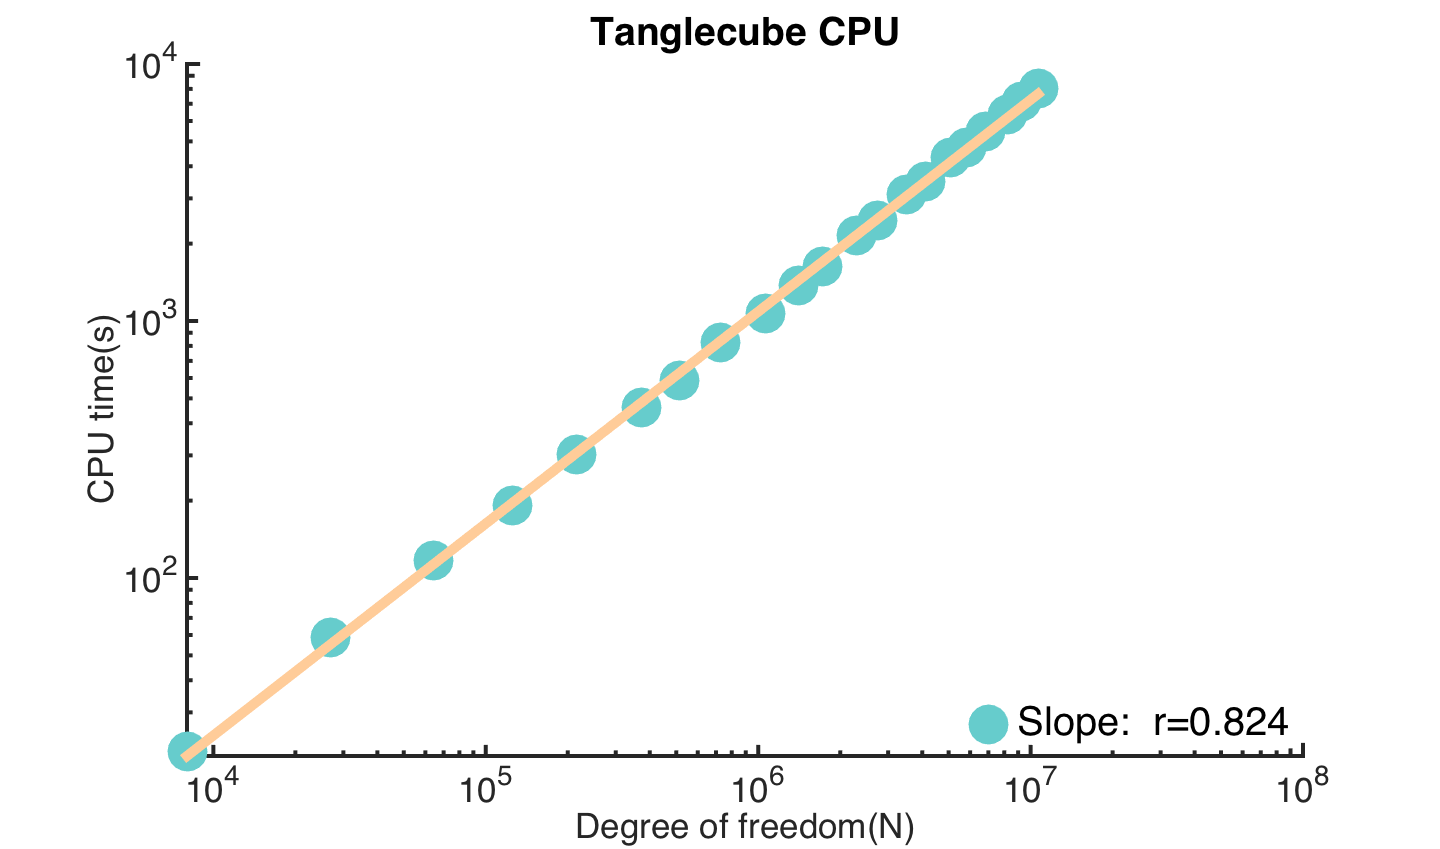
\includegraphics[width=10cm]{../figures/Tanglecube_CPU.png} & \quad & 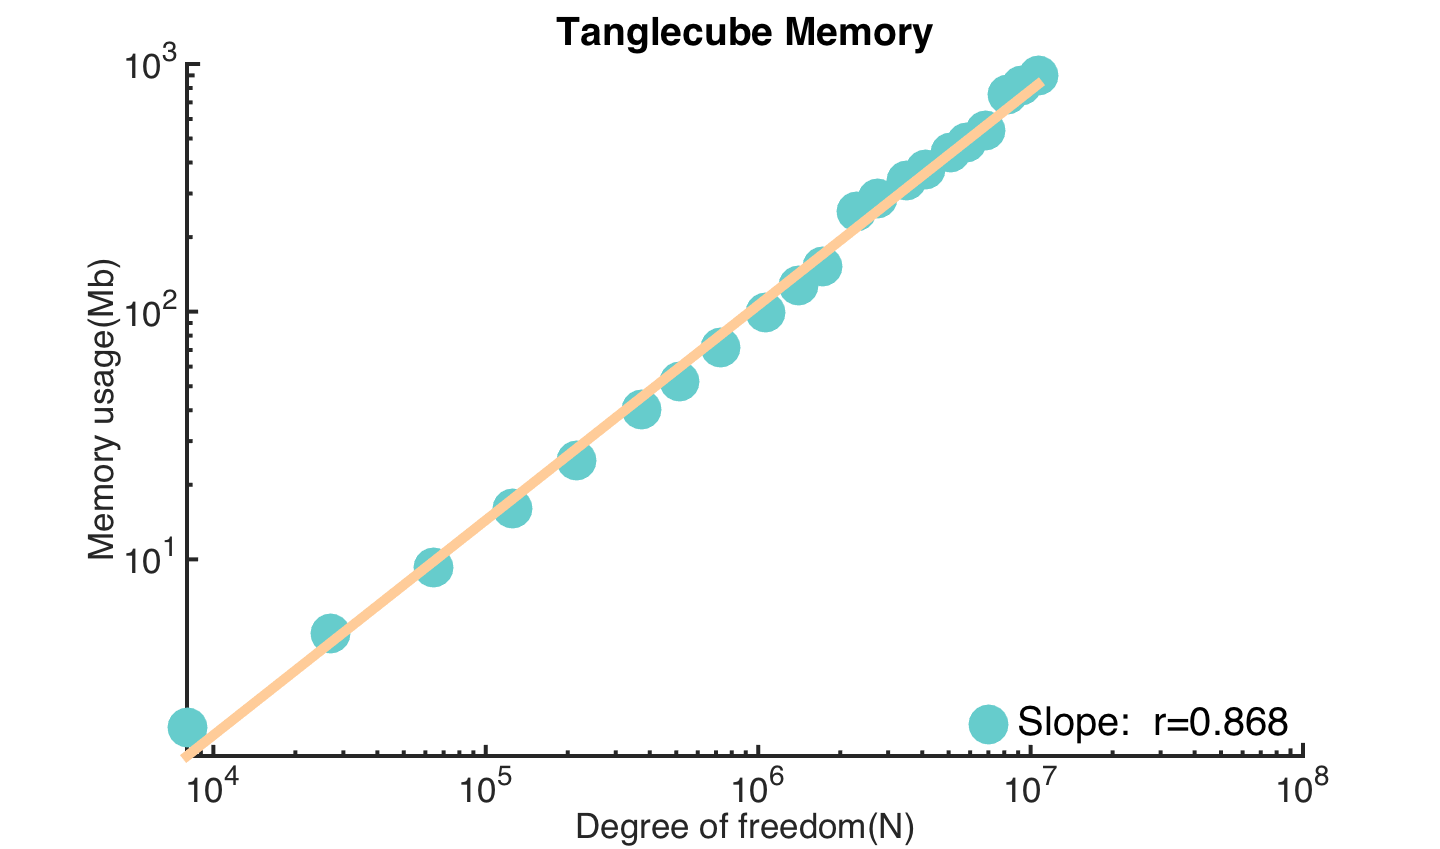
\includegraphics[width=10cm]{../figures/Tanglecube_Memory.png} \\ 
				\textbf{(a)} & \quad & \textbf{(b)} 
		\end{tabular}}
	\end{center}
	\caption{CPU time and memory usage of tanglecube (a). CPU time; (b). memory usage.}
	\label{fig:CPU_Memory_tanglecube}
\end{figure*}

%----------------------------------------------------------------------%
%                                                                      %
%                               Example 6                              %
%                                                                      %
%----------------------------------------------------------------------%

{\flushleft \bf Example 6.} The last example considers a heart-shaped interface,
which is the zero level set of 
%
\begin{equation}
S(x,y,z) = (x^{2}+\frac{9}{4}y^{2}+z^{2}-1)^{3}-x^{2}z^{3}-\frac{9}{80}y^{2}z^{3}
\end{equation}
%
embedded in the domain of dimension $[-3.99,3.99]\times[-1.99,1.99]\times[-3.99,3.99]$. The analytical solution is constructed by the formula
% 
\begin{equation} \label{analytical_eqn_3} 
u(x,y,z,t)= 
\begin{cases}
(\cos(ax)+\sin(ay)+\cos(az))\sin(t), \quad   &\mbox{in } \Omega^{-} \\
(\sin(ax)+\cos(ay)+\sin(az))\sin(t), \quad   &\mbox{in } \Omega^{+}
\end{cases}
\end{equation}
%
where $a=2$ in this example. The source term is given by
% 
%\begin{scriptsize}	
\begin{equation} 
f(x,y,z,t)= 
\begin{cases}
\alpha^{-} a^{2}(\cos(ax)+\sin(ay)+\cos(az))\sin(t)+ \\
\quad \quad \quad \quad \quad \quad \quad \quad \quad \quad (\cos(ax)+\sin(ay)+\cos(az))\cos(t), \quad   &\mbox{in } \Omega^{-} \\
\alpha^{+} a^{2}(\sin(ax)+\cos(ay)+\sin(az))\sin(t)+ \\
\quad \quad \quad \quad \quad \quad \quad \quad \quad \quad (\sin(ax)+\cos(ay)+\sin(az))\cos(t). \quad    &\mbox{in } \Omega^{+}
\end{cases}
\end{equation}
\label{source_eqn_3}
%\end{scriptsize} 
%

The significance of this example is that its interface has two singularities, one on the top and the other at the bottom, as shown in Figure \ref{fig:color_map_heart}. The singularities have not been considered in previous examples, and it is of great interest to see how well the proposed matched ADI scheme performs on this example. 
Due to the proper corner treatment, it is found that the singularities on the interface has little impact on the spatial convergence rate, as shown in Table \ref{table:heart}. 
The spatial convergence rate is close to 2 in the $L_2$ norm, and is slightly reduced 
for the $L_{\infty}$ norm. 
The temporal convergence test in Figure \ref{fig:temporal_convergence_heart}  indicates that the temporal  order is still higher than one. 
%
\begin{figure*}[!ht]	
	\begin{center}
		\resizebox{\textwidth}{!}{
			\begin{tabular}{ccc}
				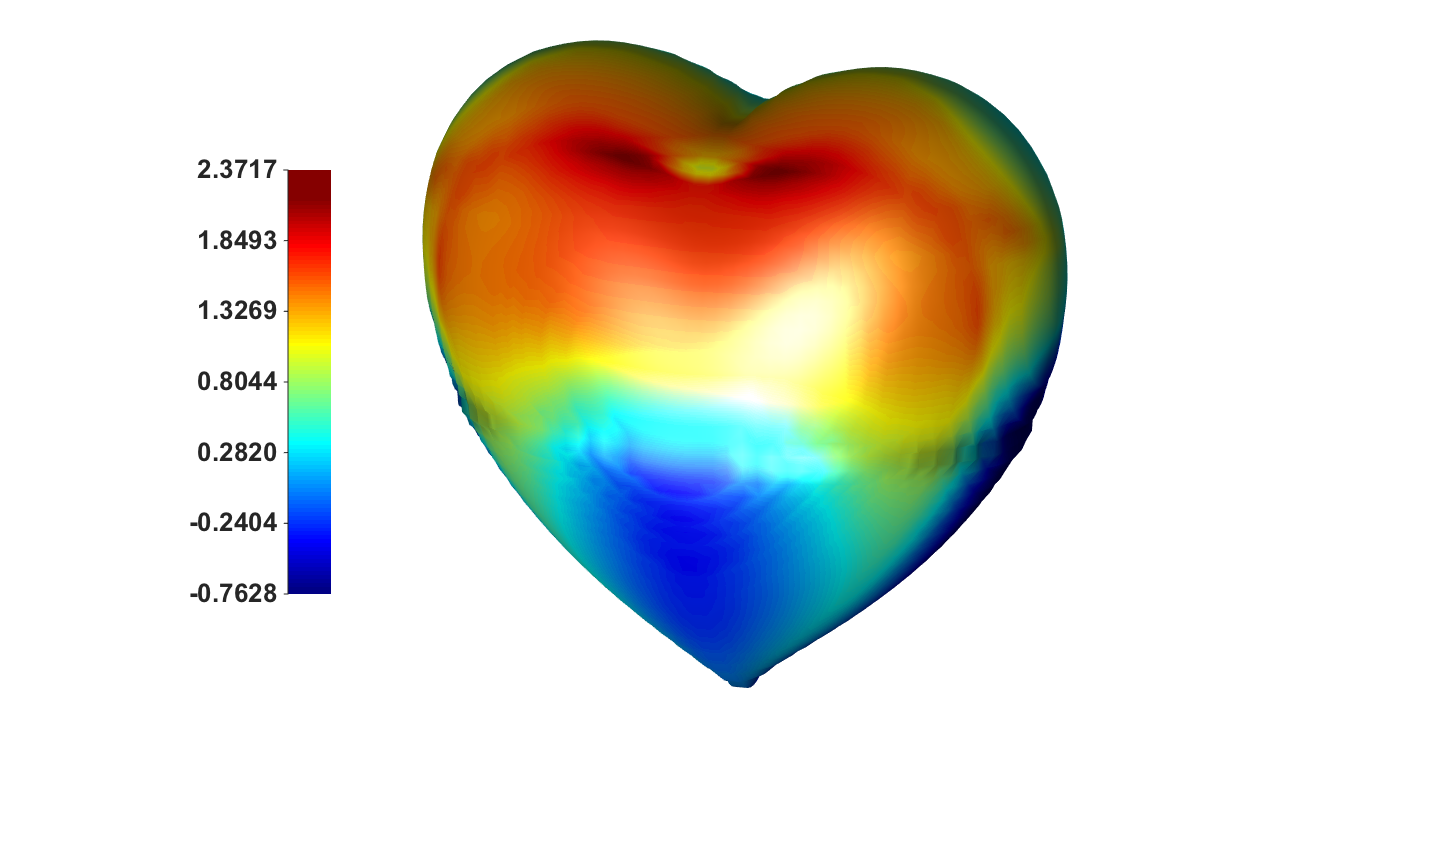
\includegraphics[width=10cm]{../figures/Heart_Solution.png} & \quad & 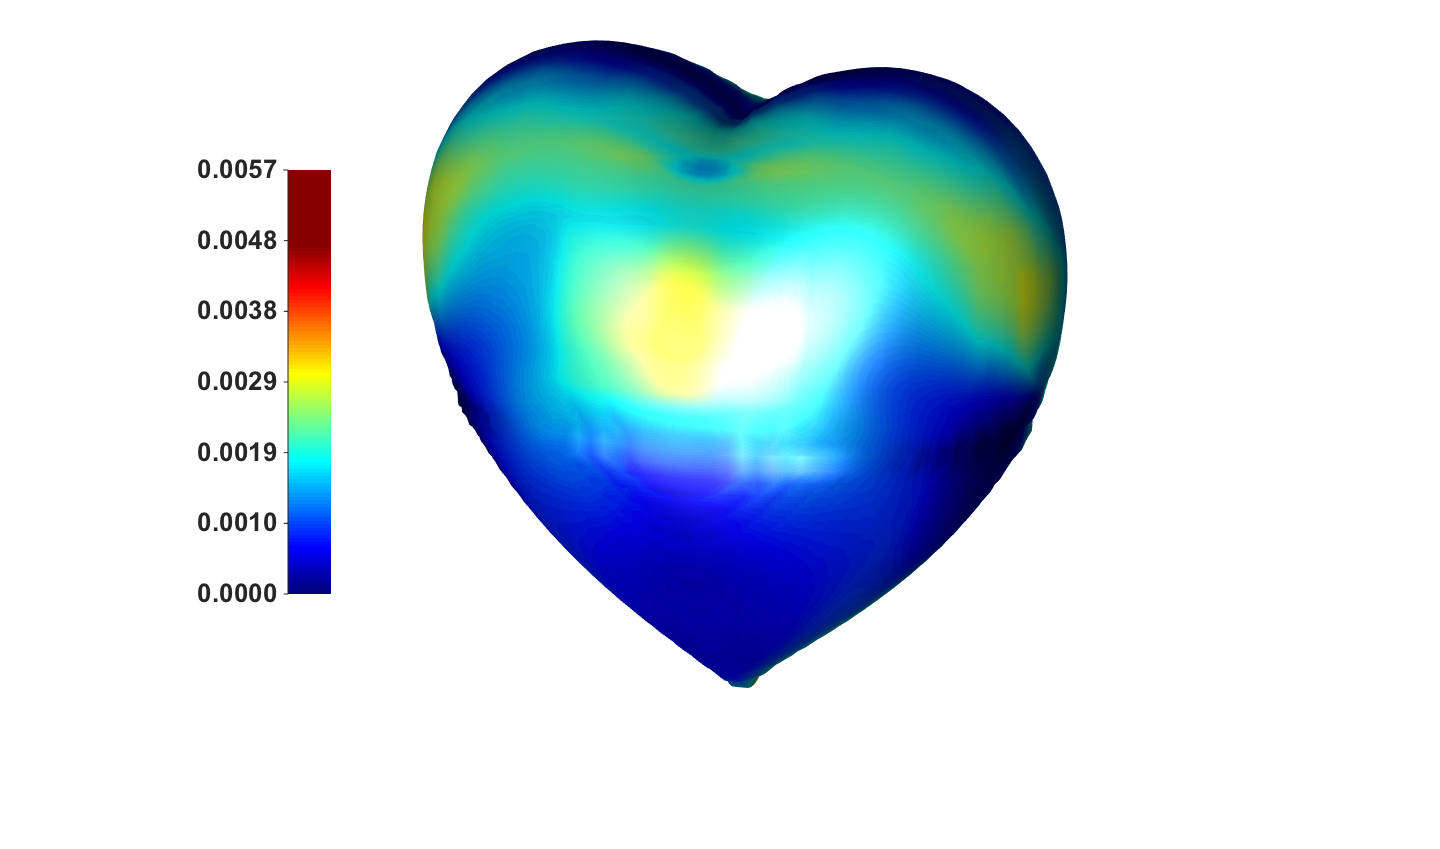
\includegraphics[width=10cm]{../figures/Heart_Error.png} \\ 
				\textbf{(a)} & \quad & \textbf{(b)} 
		\end{tabular}}
	\end{center}
	\caption{Color maps for heart surface. (a). numerical solution; (b). numerical error.}
	\label{fig:color_map_heart}
\end{figure*}
%


%\noindent
\begin{table}
	\centering
	\renewcommand{\arraystretch}{1.0}% Tighter
	\resizebox{\textwidth}{!}{
		\tiny
		\begin{tabular}{c @{\hskip 8mm} cccccccc @{}}\midrule
			\multirow{2}{*}{$[N_{x},N_{y},N_{z}]$} 				%&\multicolumn{5}{c}{Example 6} \\ 
			%\cmidrule{2-6}
			&\multicolumn{2}{c}{$L_{\infty}$}  & \phantom{abc}
			&\multicolumn{2}{c}{$L_2$} \\ 
			\cmidrule{2-3} \cmidrule{5-6}
			&\multicolumn{1}{c}{Error}  &\multicolumn{1}{c}{Order}  & \phantom{abc} 
			&\multicolumn{1}{c}{Error}  &\multicolumn{1}{c}{Order} \\
			\hline
			$[20,20,20]$      & 1.456e-01  &        & & 3.560e-02  &      \\
			$[40,40,40]$      & 4.490e-02  & 1.70   & & 8.364e-03  & 2.09 \\
			$[80,80,80]$      & 2.158e-02  & 1.06   & & 2.073e-03  & 2.01 \\
			$[160,160,160]$   & 5.701e-03  & 1.92   & & 5.186e-04  & 2.00 \\
			\hline
	\end{tabular}}
	\captionof{table}{Spatial convergence for heart surface.}
	\label{table:heart}
\end{table}
%
%
\begin{figure*}[!tb] 
	\centering
	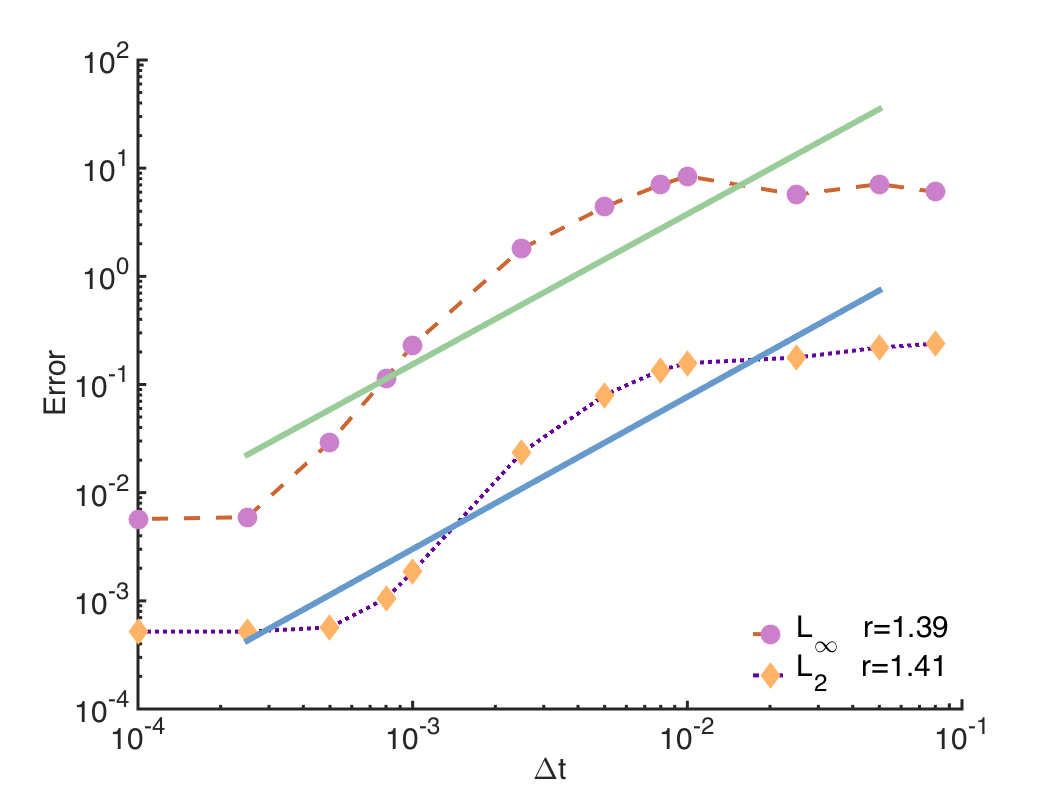
\includegraphics[width=12cm]{../figures/Heart_Time.png}
	\captionof{figure}{Temporal convergence for heart surface.}
	\label{fig:temporal_convergence_heart}
\end{figure*}
%
\begin{figure*}[!ht]	
	\begin{center}
		\resizebox{\textwidth}{!}{
			\begin{tabular}{ccc}
				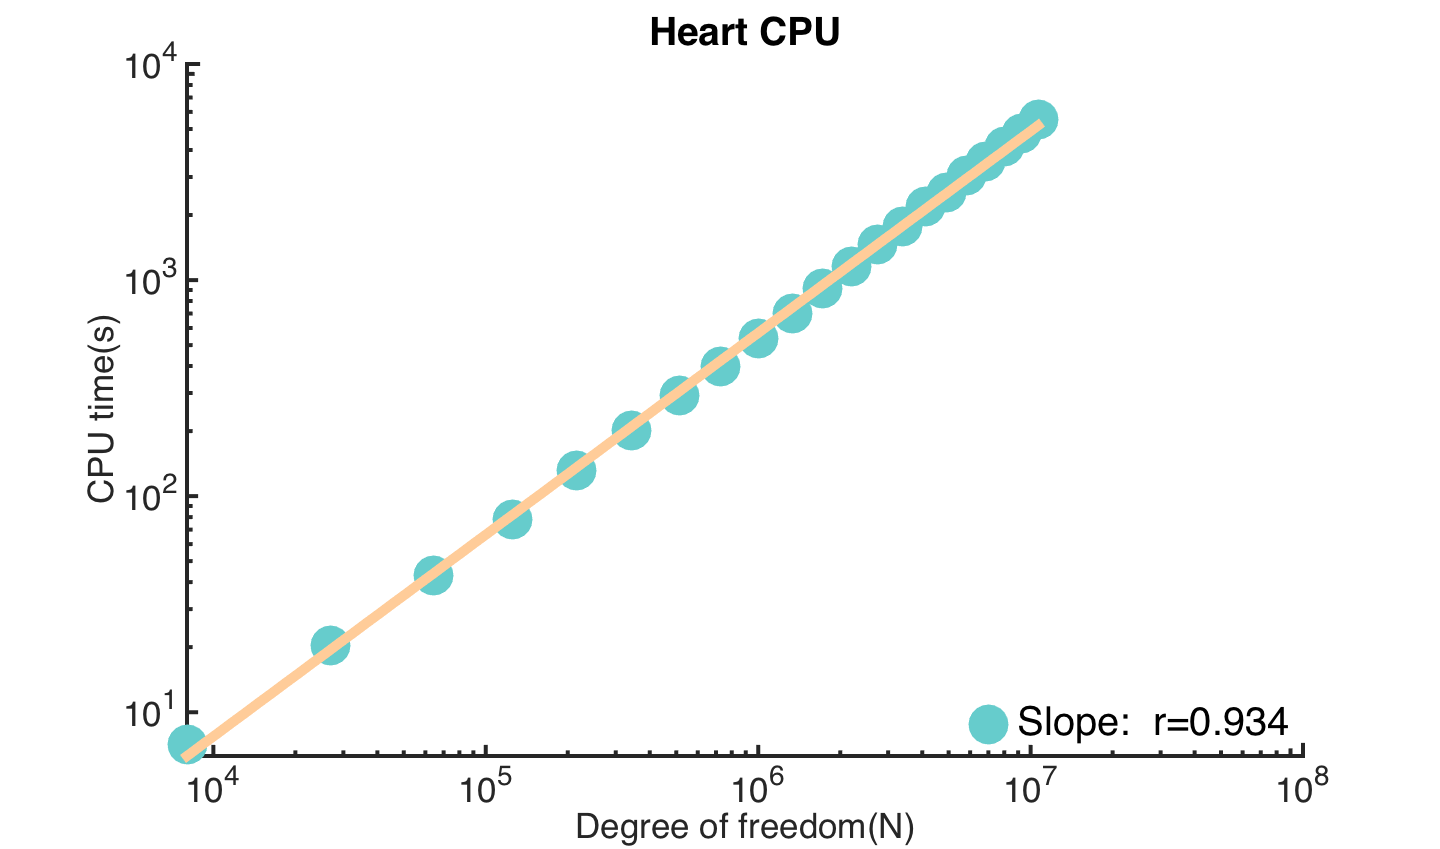
\includegraphics[width=10cm]{../figures/Heart_CPU.png} & \quad & 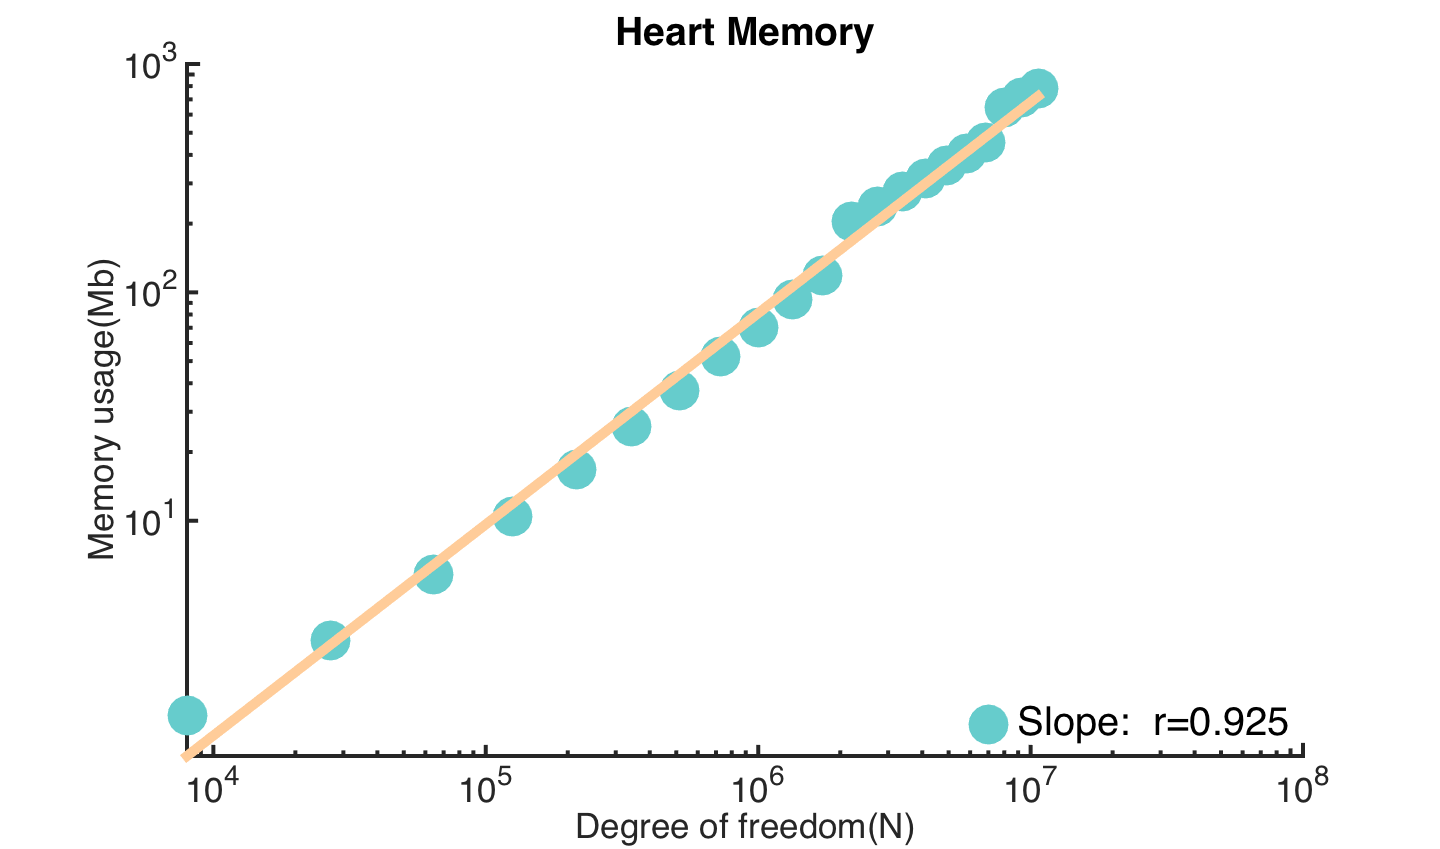
\includegraphics[width=10cm]{../figures/Heart_Memory.png} \\ 
				\textbf{(a)} & \quad & \textbf{(b)} 
		\end{tabular}}
	\end{center}
	\caption{CPU time and memory usage of heart (a). CPU time; (b). memory usage.}
	\label{fig:CPU_Memory_heart}
\end{figure*}
%
The CPU time and memory usage for this example are reported in Figure \ref{fig:CPU_Memory_heart}, with the same setting as in Example 5. Again both of them are found to be linearly scaled with a slope rate $r=0.934$ and $r=0.925$. The 3D matched ADI method is founded to be stable for the present example with singularities, which is demonstrated in Figure \ref{fig:stability_heart}. By considering a very large time step $\Delta t=10$, we calculate $N_x=N_y=N_z=20,40,80,160$ in each direction and choose the stopping time varying from $10^{3}$ to $10^{5}$. It can be seen that the errors do not grow with respect to the time for all mesh sizes.  Great stability has been observed in all tested cases.

\begin{figure}[!ht] 
	\centering
	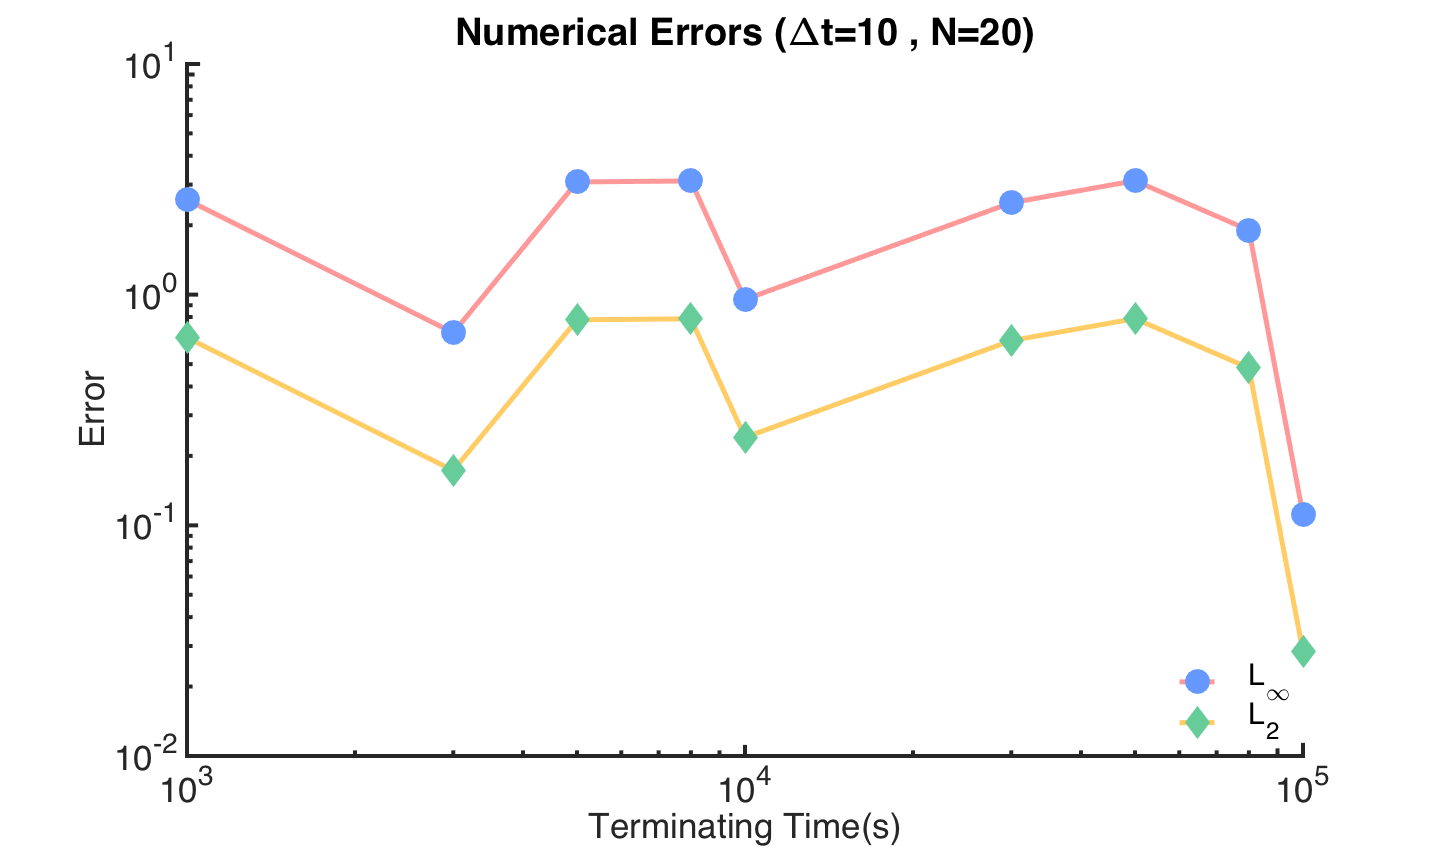
\includegraphics[width=8cm]{../figures/Heart_Stability_20.png}\quad
	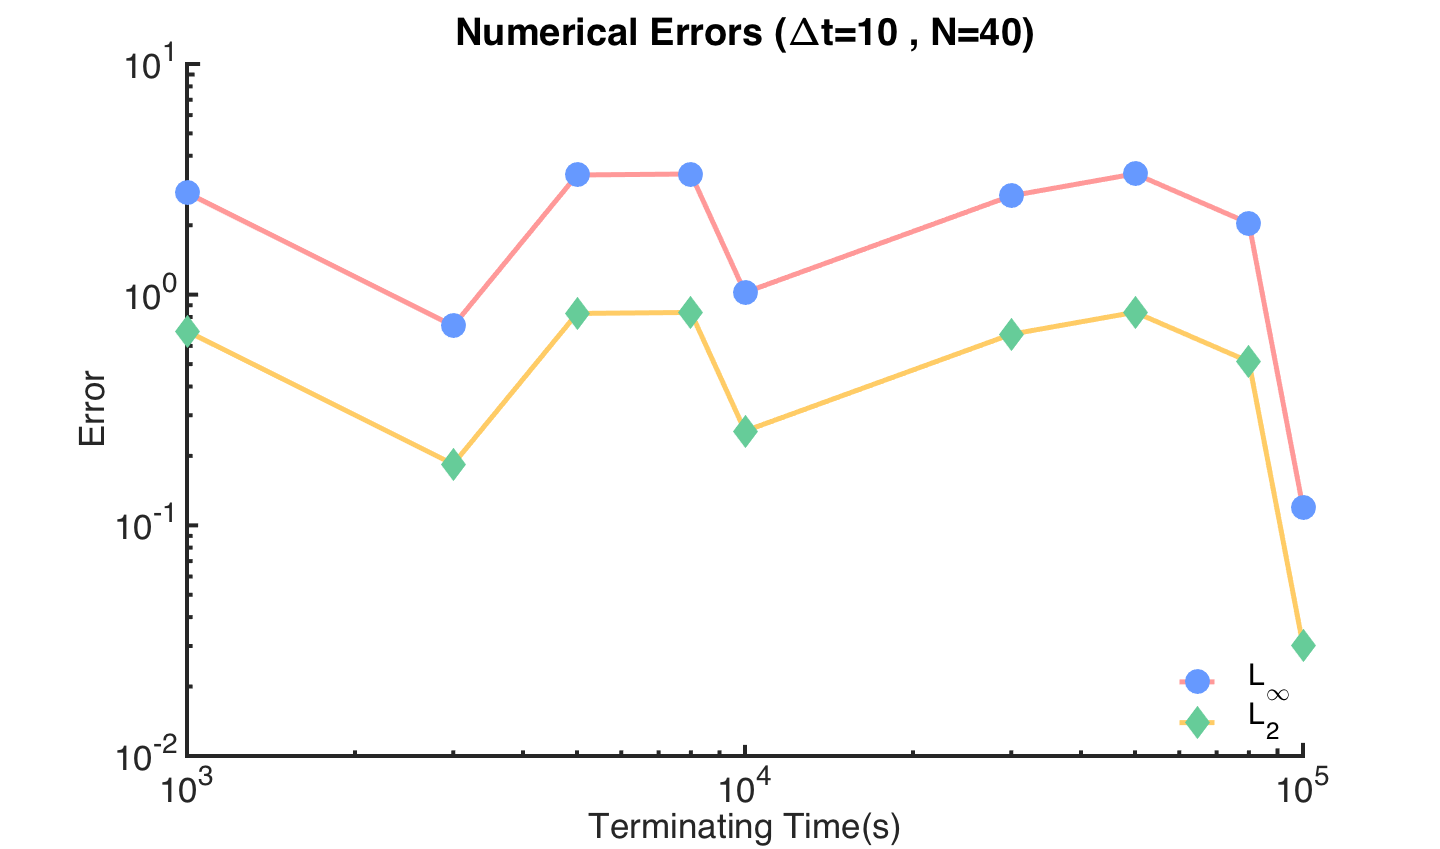
\includegraphics[width=8cm]{../figures/Heart_Stability_40.png}
	\medskip
	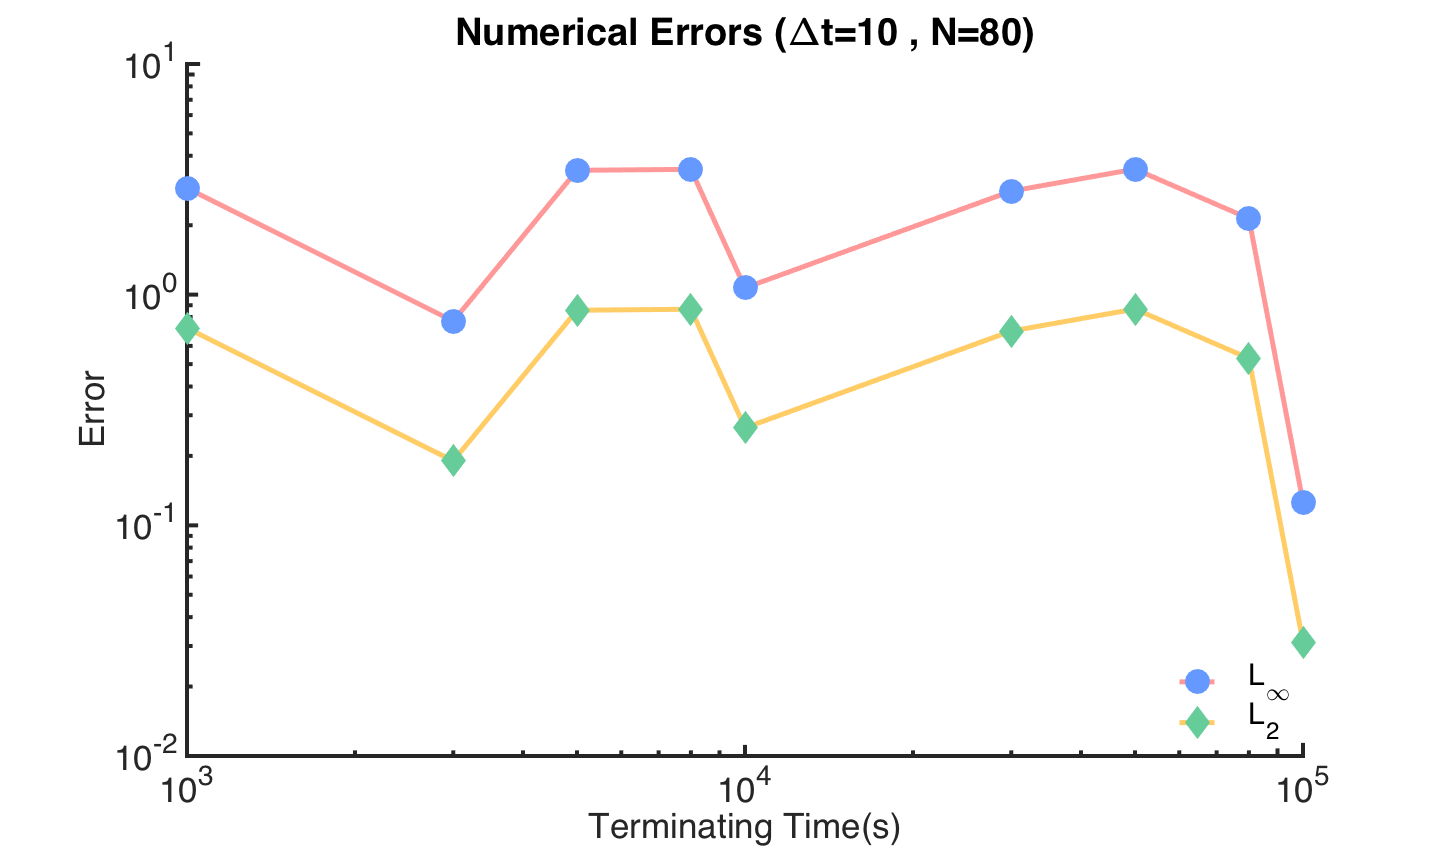
\includegraphics[width=8cm]{../figures/Heart_Stability_80.png}\quad
	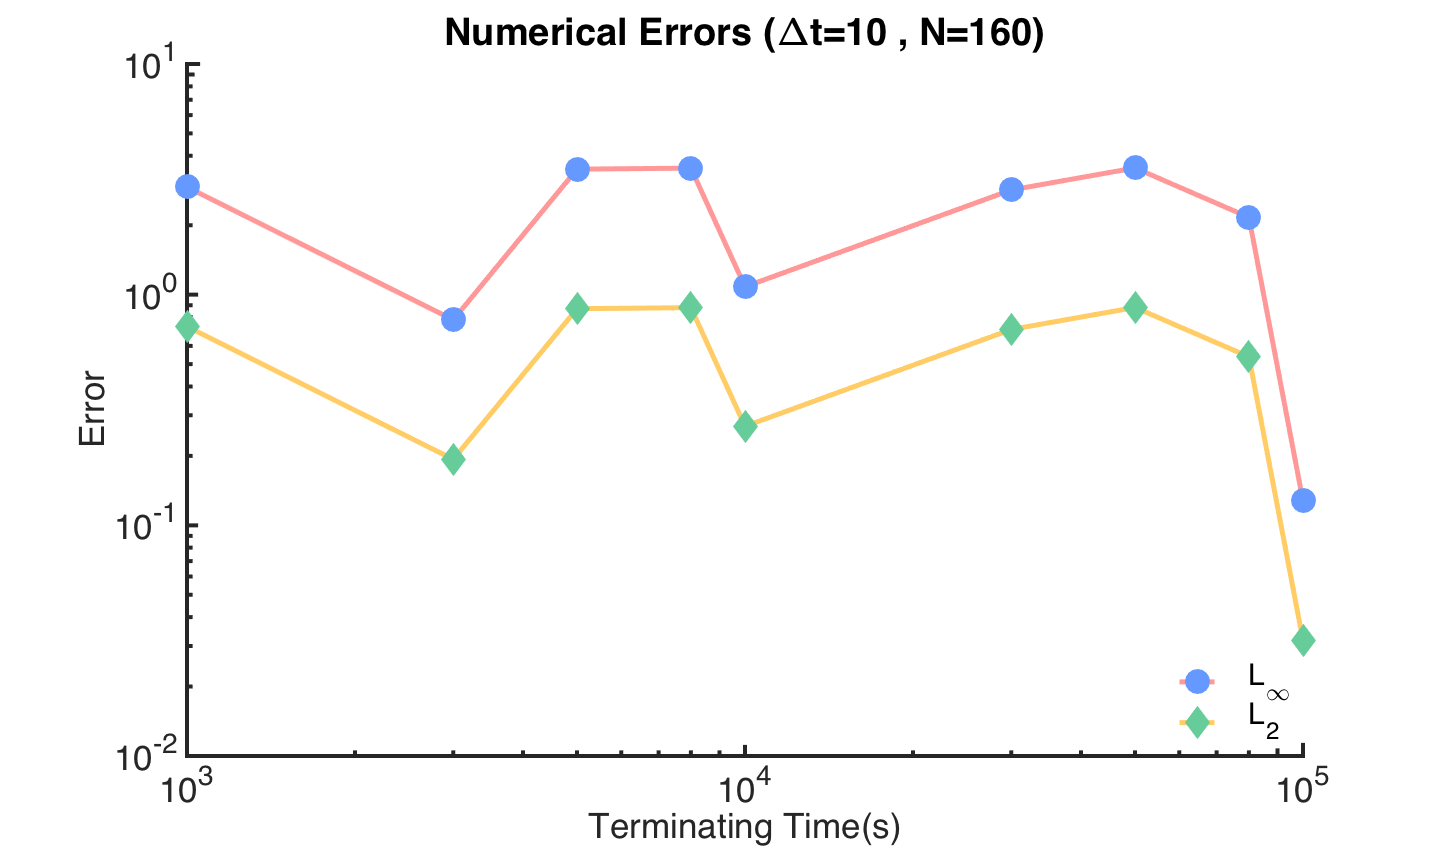
\includegraphics[width=8cm]{../figures/Heart_Stability_160.png}
	\caption{Stability test for the heart surface in Example 6.}
	\label{fig:stability_heart}
\end{figure}



\section{Comparison of time splitting methods with variable diffusion coefficients}
In this section, we focus on efficiency and accuracy comparison of a total of eight methods, two spatial methods coupled with four temporal methods. Spatially, two variations of matched interface and boundary (MIB) methods are considered, to be simple, since GFM is essentially equivalent to MIB-L1 method with less accurate derived jump condition. For temporal methods, we consider all the four methods Douglas-Rachford alternating direction implicit (ADI) method, locally one-dimensional implicit Euler (LOD-IE), locally one-dimensional Crank-Nicolson (LOD-CN) and Trapezoidal Splitting (TS) method in chapter 3. We coupled the two spacial methods and the four temporal methods altogether in the experiments. Consequently, to be simple we call these eight methods ADI-L1, ADI-L2, LODIE-L1, LODIE-L2, LODCN-L1, LODCN-L2, TS-L1 and TS-L2. Only variable diffusion coefficients is considered in the experiments since piecewise constant diffusion coefficients is just a special case. The code is written in C++ and compiled with GCC 4.8.5 compiler and C++11 standard, "vector" in C++ STL has been used as the major data structure taking advantage of the guaranteed contiguous memory allocated. Reported CPU time is recorded on the master node of SGI Ultraviolet in Alabama Supercomputer Center with a single Xeon E5-4640 CPU core operating at 2.4 GHz clock speed.

Three types of variable coefficients are taken into consideration, different functions have different properties. It would be better to test the behavior between different algorithms based on distinct analytical solutions, shapes and types of variable coefficients. The first type of variable coefficient is rational function, 
\begin{equation} \label{beta_1}
\alpha(x, y, z)= 
\begin{cases}
\frac{1}{x^2 + y^2 + z^2 + 1} + 1,  &\mbox{in } \Omega^{-} \\
-\frac{1}{x^2 + y^2 + z^2 + 1} + 2.  &\mbox{in } \Omega^{+}
\end{cases}
\end{equation}
The second type of variable coefficient is trigonometric function,
\begin{equation} \label{beta_2}
\alpha(x, y, z)= 
\begin{cases}
sin(x + y + z) +2,   &\mbox{in } \Omega^{-} \\
-cos(x + y + z) + 2.  &\mbox{in } \Omega^{+}
\end{cases}
\end{equation}
The third type of variable coefficient is Gaussian function
\begin{equation} \label{beta_3}
\alpha(x, y, z)= 
\begin{cases}
e^{\frac{x^2}{{\sigma_x}^2} + \frac{x^2}{{\sigma_x}^2} + \frac{x^2}{{\sigma_x}^2}},  &\mbox{in } \Omega^{-} \\
e^{\frac{x^2}{{\overline{\sigma}_x}^2} + \frac{x^2}{{\overline{\sigma}_y}^2} + \frac{x^2}{{\overline{\sigma}_z}^2}}.  &\mbox{in } \Omega^{+}
\end{cases}
\end{equation}
with amplitude as constant 1, and variance $\mu = 0$, standard deviation $\sigma_x=\sigma_y=\sigma_z=3$ in the region $\Omega^{-}$ and ${\overline{\sigma}_x}={\overline{\sigma}_y}={\overline{\sigma}_z}=4$ in the region $\Omega^{+}$ in all three directions.
%----------------------------------------------------------------------%
%                                                                      %
%                               Example 7                              %
%                                                                      %
%----------------------------------------------------------------------%

{\flushleft \bf Example 7.} Consider a simple sphere surface
% 
\begin{equation} \label{sphere}
S(x,y,z) = x^{2} + y^{2} + z^{2} -1.
\end{equation}
%
with analytical solution (\ref{analytical_eqn_1}) with $a=2$. The source term depends on the first type of variable coefficient which is a pair of rational functions from (\ref{beta_1}) based on the grid locations. The zeroth order jump condition on the interface is kept as time-dependent and the first order jump condition is time-independent. The computational domain is fixed to be $[-3.99,3.99]\times[-1.99,1.99]\times[-1.99,1.99]$. 

%---------------------------- sphere type 1 ---------------------------------------
%
\begin{figure}[!tb] 
	\centering
	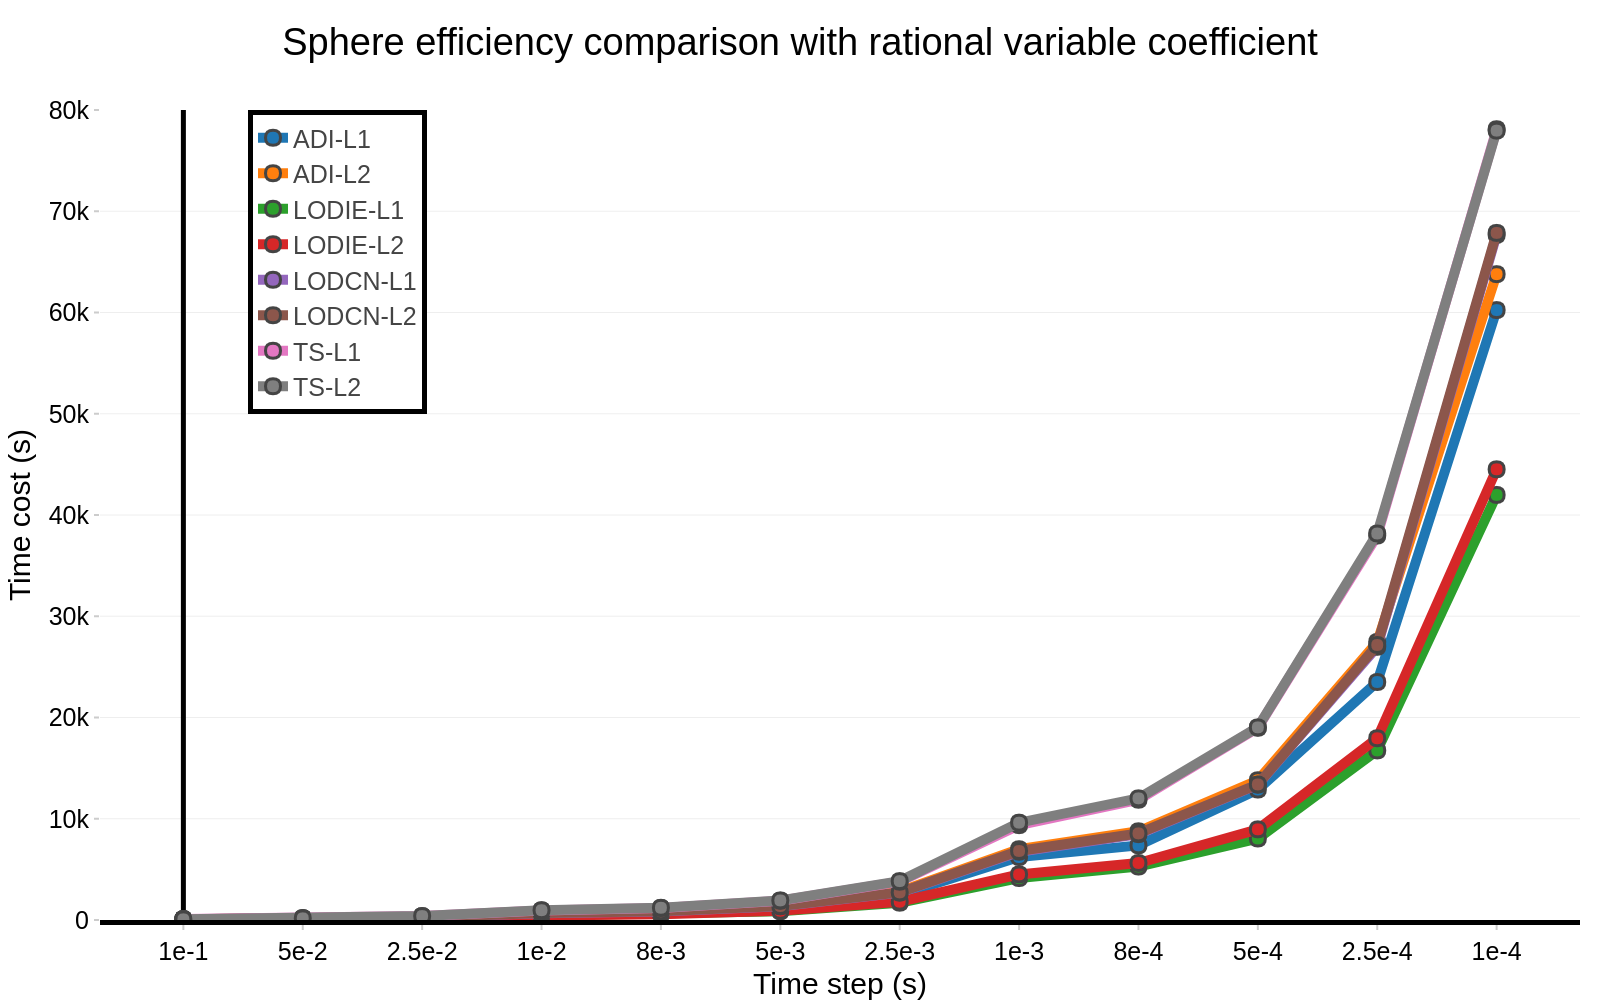
\includegraphics[width=13cm]{../figures/sphere_efficiency_1.png}
	\captionof{figure}{Sphere efficiency comparison with rational type variable coefficient.}
	\label{fig:sphere_efficiency_1}
\end{figure}

\begin{figure}[!tb] 
	\centering
	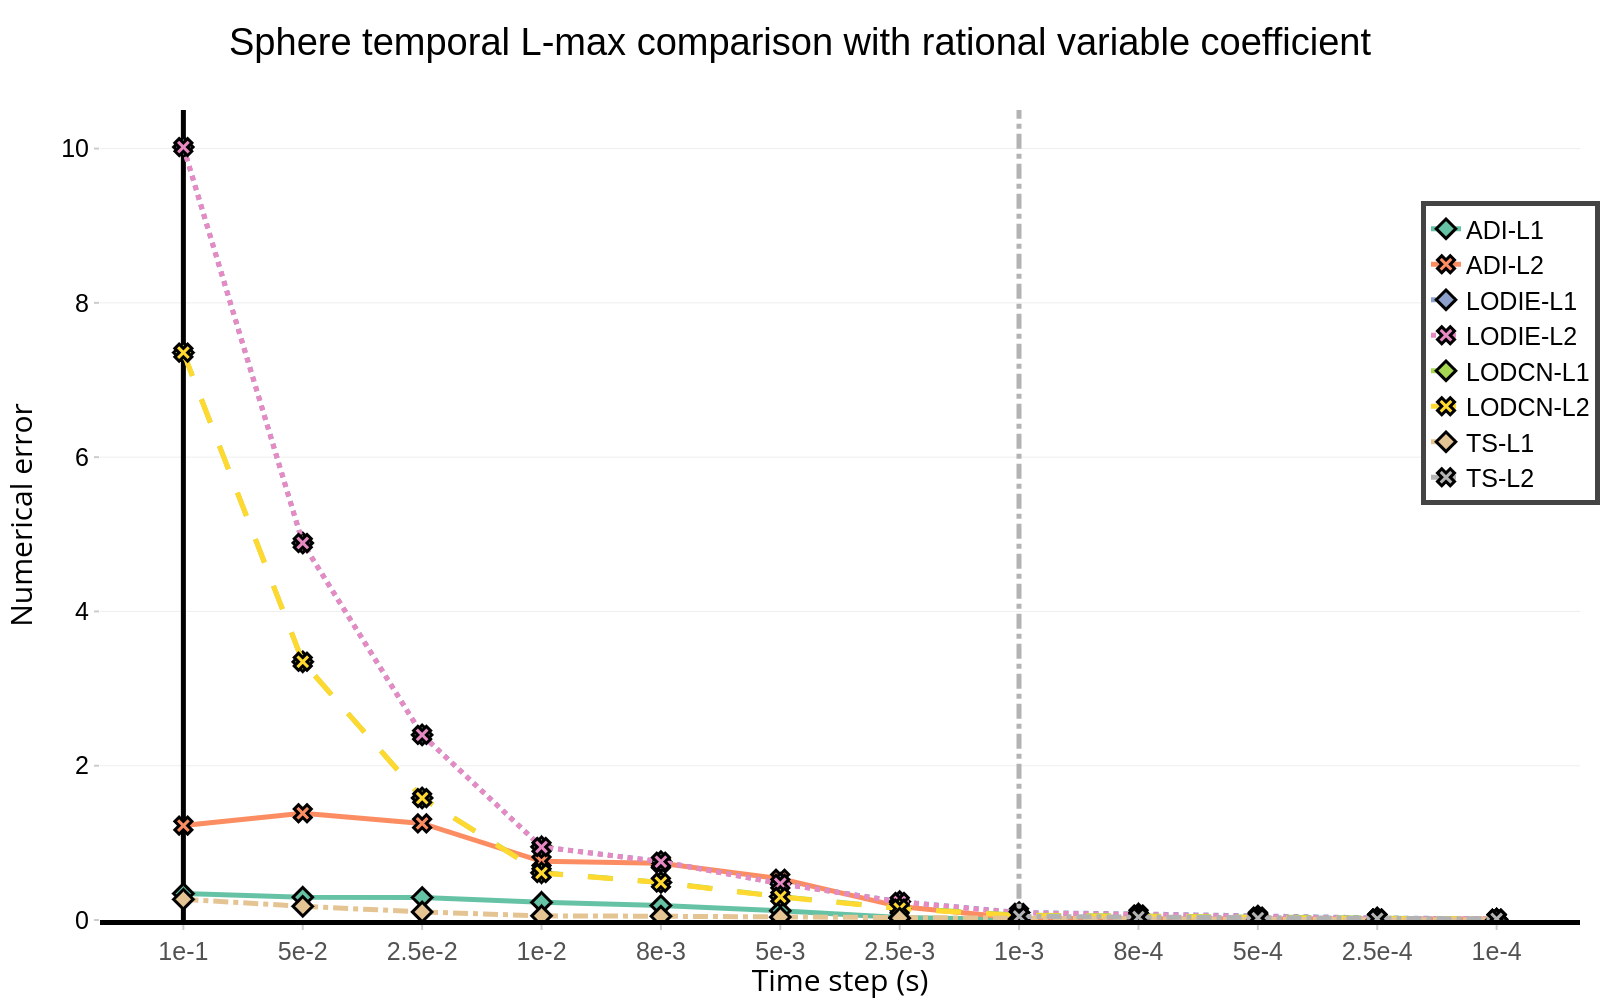
\includegraphics[width=13cm]{../figures/sphere_lmax_1.png}
	\captionof{figure}{Temporal $L_{\infty}$ error for sphere interface with rational type variable coefficient.}
	\label{fig:sphere_temporal_lmax_type_1}
\end{figure}

\begin{figure}[!tb] 
	\centering
	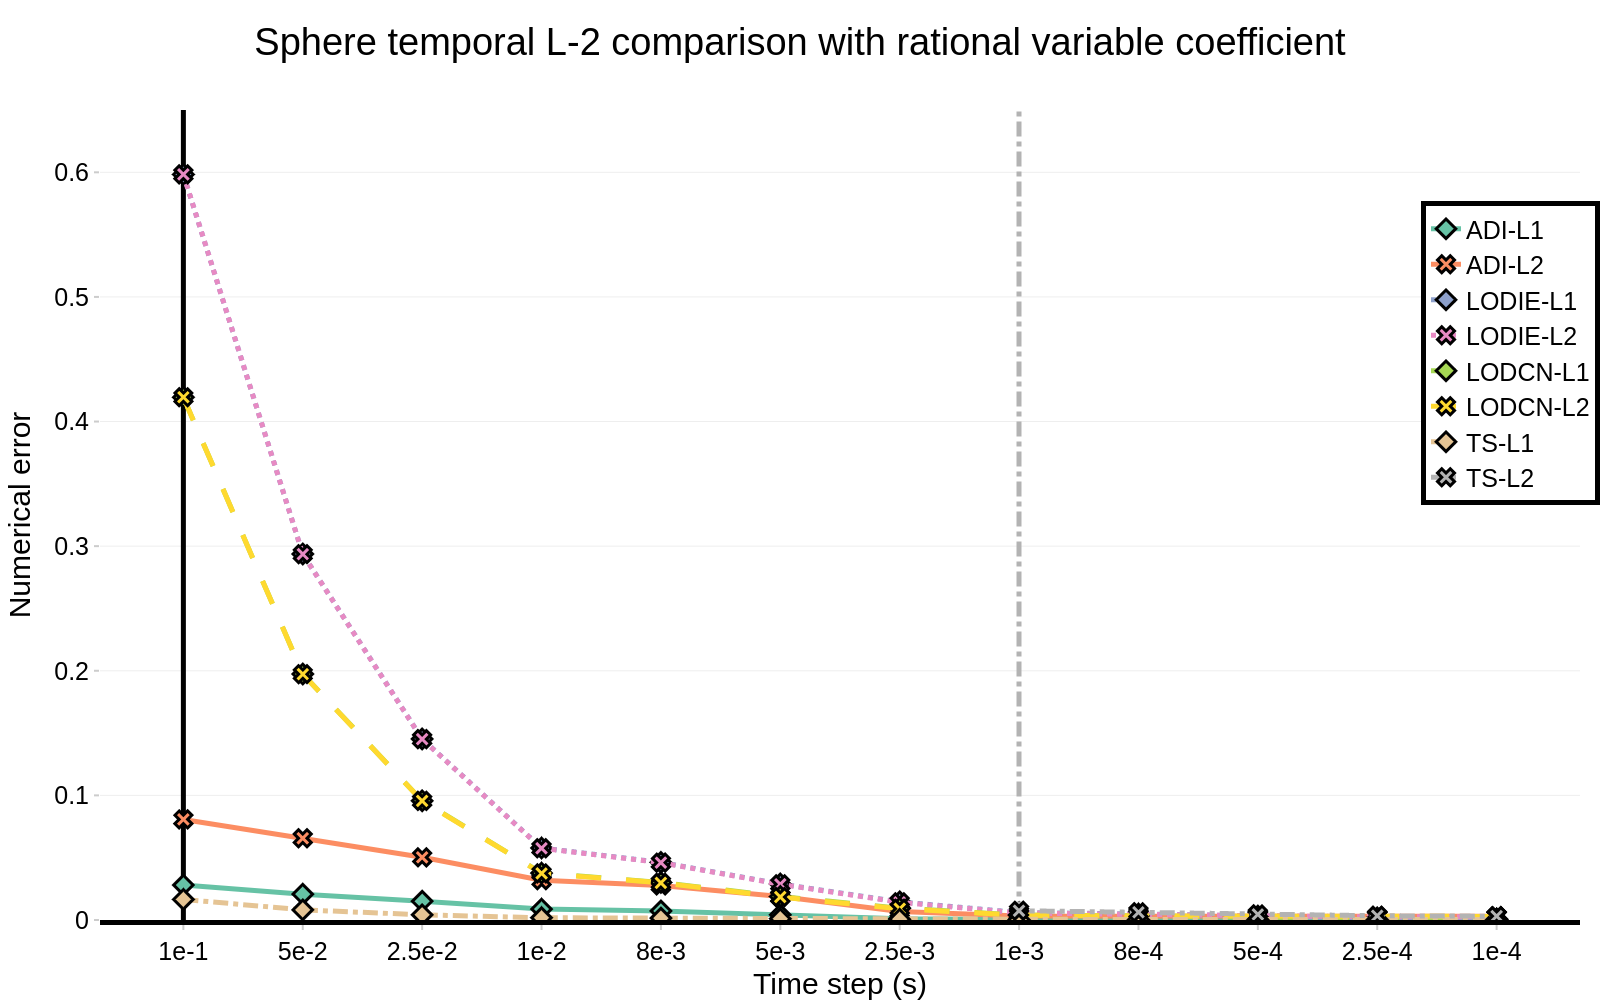
\includegraphics[width=13cm]{../figures/sphere_l2_1.png}
	\captionof{figure}{Temporal $L_{2}$ error for sphere interface with rational type variable coefficient.}
	\label{fig:sphere_temporal_l2_type_1}
\end{figure}

\begin{figure}[!tb] 
	\centering
	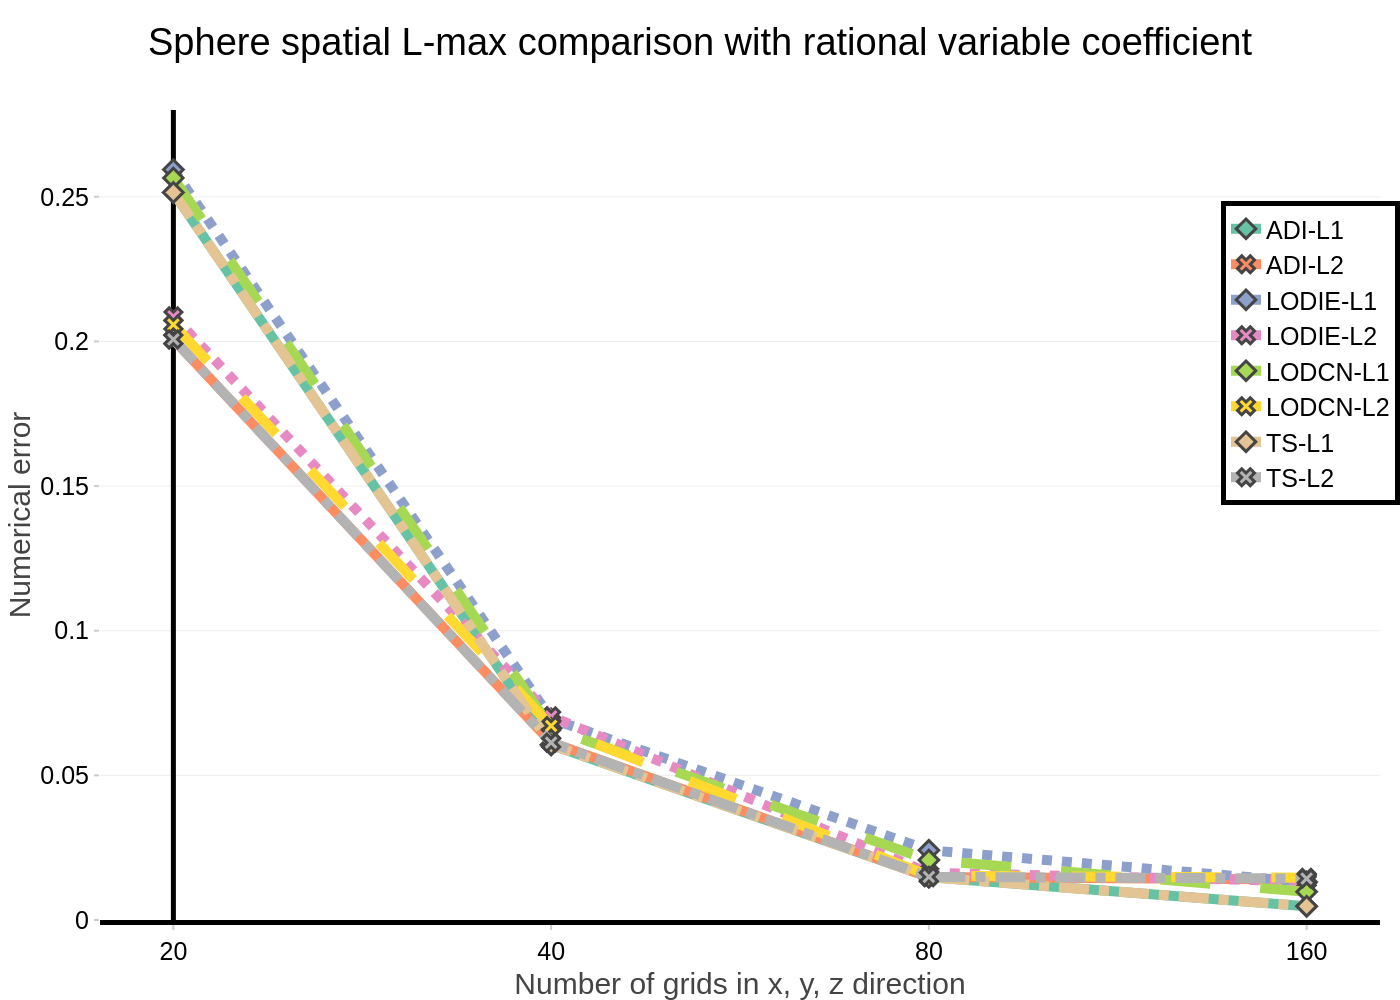
\includegraphics[width=13cm]{../figures/spatial_sphere_lmax_1.png}
	\captionof{figure}{Spatial $L_{\infty}$ error for sphere interface with rational type variable coefficient.}
	\label{fig:sphere_spatial_lmax_type_1}
\end{figure}

\begin{figure}[!tb] 
	\centering
	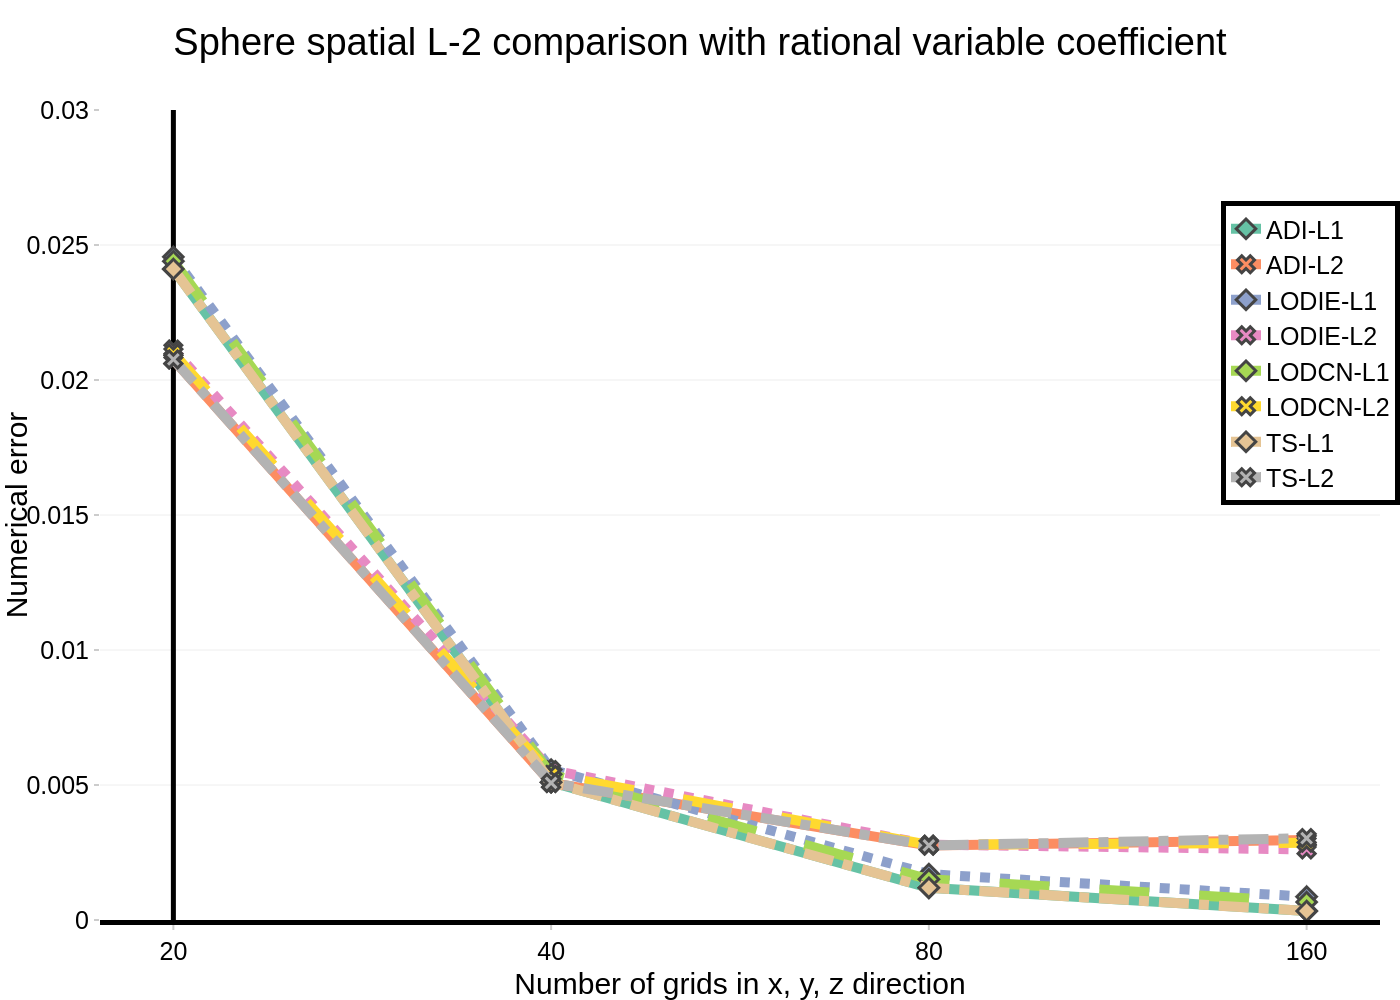
\includegraphics[width=13cm]{../figures/spatial_sphere_l2_1.png}
	\captionof{figure}{Spatial $L_{2}$ error for sphere interface with rational type variable coefficient.}
	\label{fig:sphere_spatial_l2_type_1}
\end{figure}
%
A efficiency comparison is performed in Figure \ref{fig:sphere_efficiency_1}, the cost of the most expensive algorithm are about two times expensive than the cheapest algorithm. Not surprisingly, TS-L1 and TS-L2 methods are the most expensive one due to more operations in Trapezoidal splitting algorithm. Meanwhile, it is easy to tell that LODIE-L1 and LODIE-L2 are the cheapest algorithms. For temporal numerical error, regards both $L_2$ and $L_{\infty}$, in Figure \ref{fig:sphere_temporal_lmax_type_1} and \ref{fig:sphere_temporal_l2_type_1},the spacial size are fixed at 160 in all three x, y, z directions. All methods are stable with large time step except TS-L2, as we mentioned in previous chapter, the scheme of Trapezoidal splitting method used in this work has been modified at the fifth step, it could be a potential reason of the instability. However, TS-L1 is stable for all different time steps, which implies that different MIB scheme could also generate some instability issue based on some specific temporal method. A variation of MIB method leads to a different matrix structure when solving the linear system which might essentially affect the stability. Other than the stability issue with TS-L2, almost all methods stop perform first order convergence rate after some time step. The variable diffusion coefficient somehow restrict the performance of first order convergence no matter what temporal algorithm are adopted. Spatially, in Figure \ref{fig:sphere_spatial_lmax_type_1} and \ref{fig:sphere_spatial_l2_type_1}, time step are picked at $\Delta{t}=1e-4$, with grid size vary from 20 to 160, none of $L_2$ and $L_{\infty}$ can perform the overall 2nd order convergence rate in space. The big difference between different algorithms at the beginning is that all methods using MIB-L2 scheme performs slightly more accurate than the methods using MIB-L1 scheme. As grid mesh become finer and finer, the gap are narrowed down expeditiously. For $L_2$ numerical error, with the finest mesh grid 160, the interesting thing is, all methods using MIB-L1 scheme are converged to a magnitude of $\Delta{t}=1e-4$ and the methods using MIB-L2 scheme only converge to a magnitude of $\Delta{t}=1e-3$.


%----------------------------------------------------------------------%
%                                                                      %
%                               Example 8                              %
%                                                                      %
%----------------------------------------------------------------------%

{\flushleft \bf Example 8.} The simple sphere surface is still adopted from (\ref{sphere}) with analytical solution (\ref{analytical_eqn_1}) with $a=2$ in a computational domain $[-3.99,3.99]\times[-1.99,1.99]\times[-1.99,1.99]$. A trigonometric type of variable coefficient is constructed as (\ref{beta_2}).
%---------------------------- sphere type 2 ---------------------------------------
%
\begin{figure}[!tb] 
	\centering
	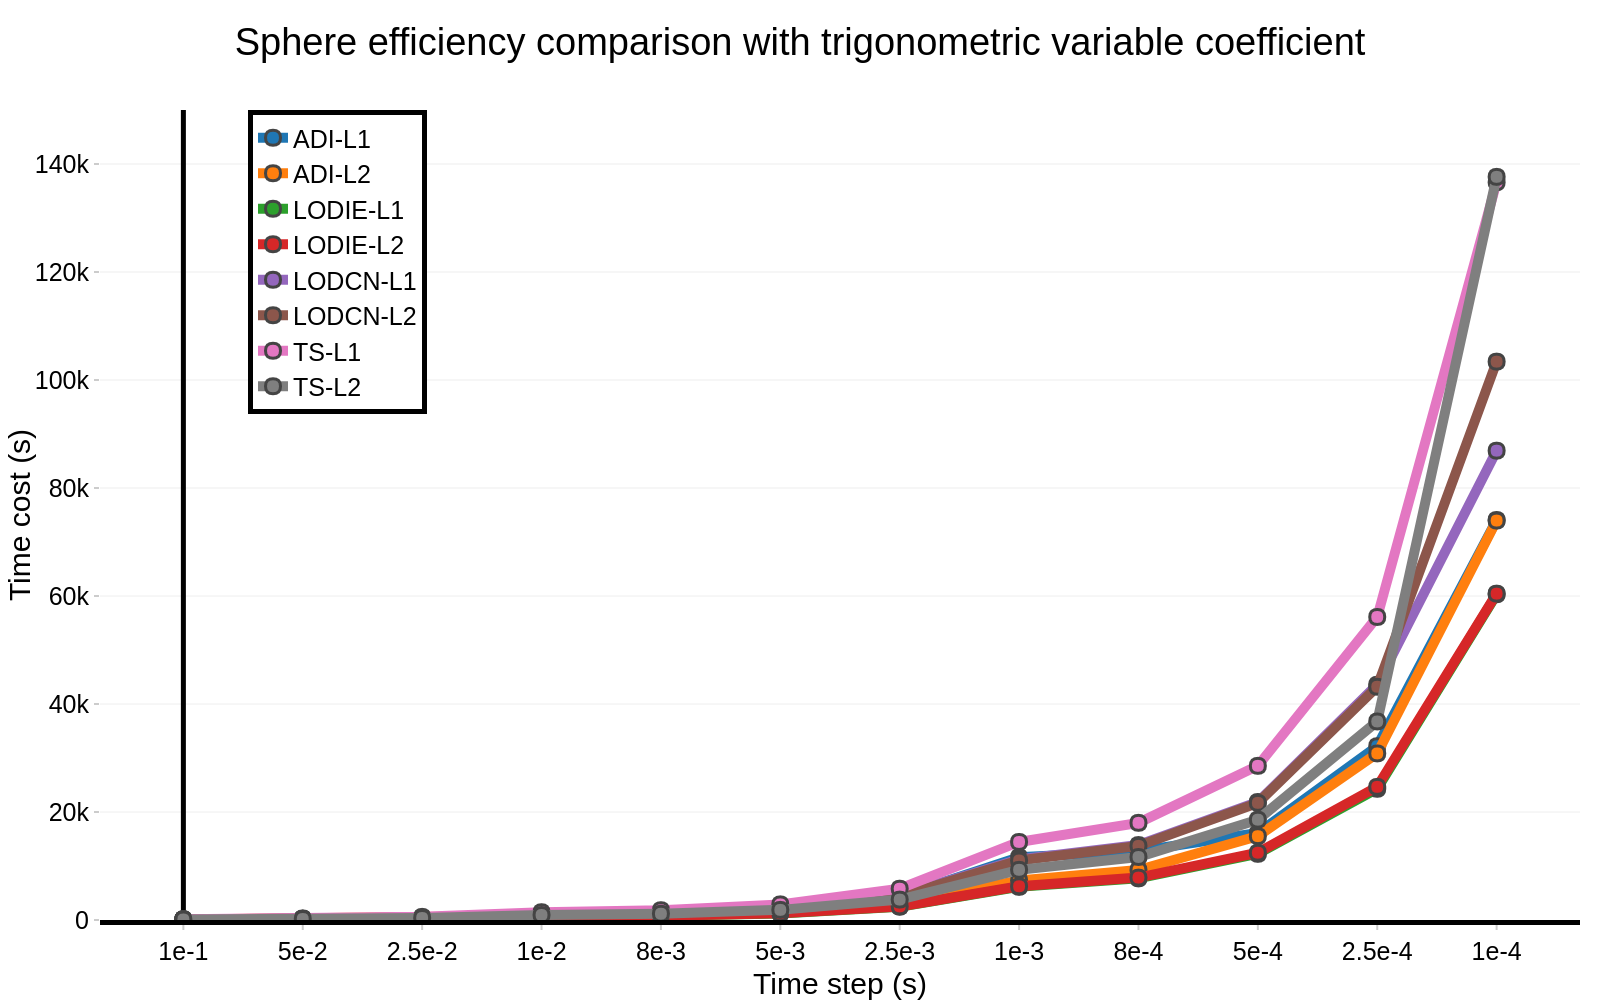
\includegraphics[width=13cm]{../figures/sphere_efficiency_2.png}
	\captionof{figure}{Sphere efficiency comparison with trigonometric type variable coefficient.}
	\label{fig:sphere_efficiency_2}
\end{figure}

\begin{figure}[!tb] 
	\centering
	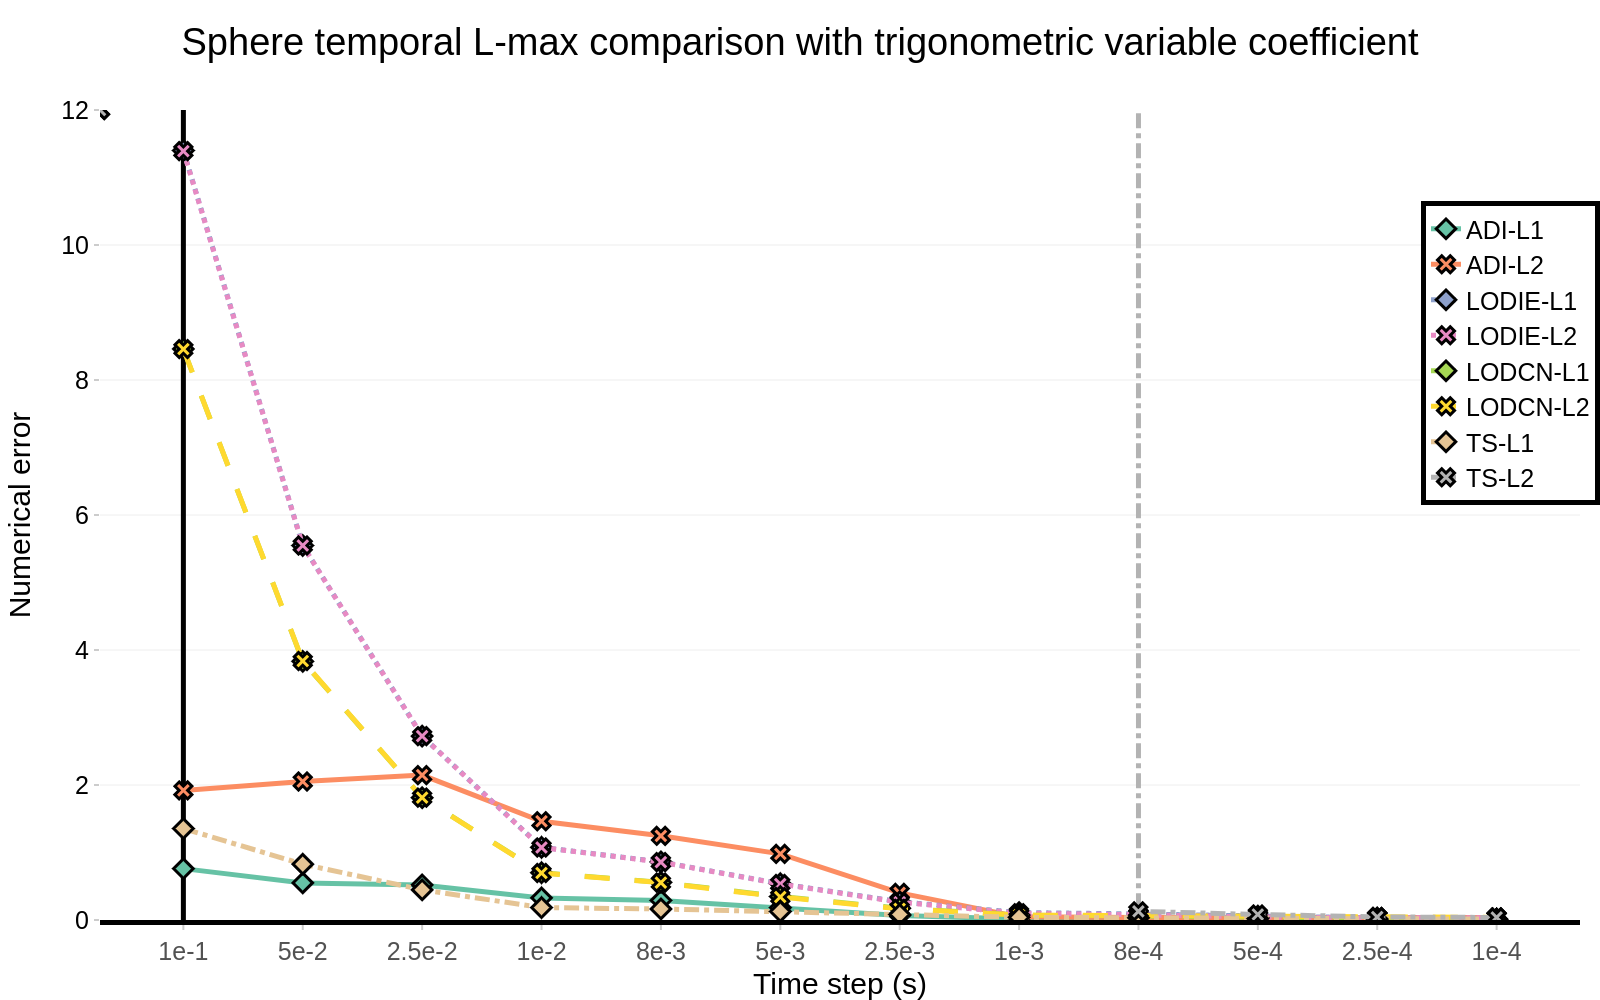
\includegraphics[width=13cm]{../figures/sphere_lmax_2.png}
	\captionof{figure}{Temporal $L_{\infty}$ error for sphere interface with trigonometric type variable coefficient.}
	\label{fig:sphere_temporal_lmax_type_2}
\end{figure}

\begin{figure}[!tb] 
	\centering
	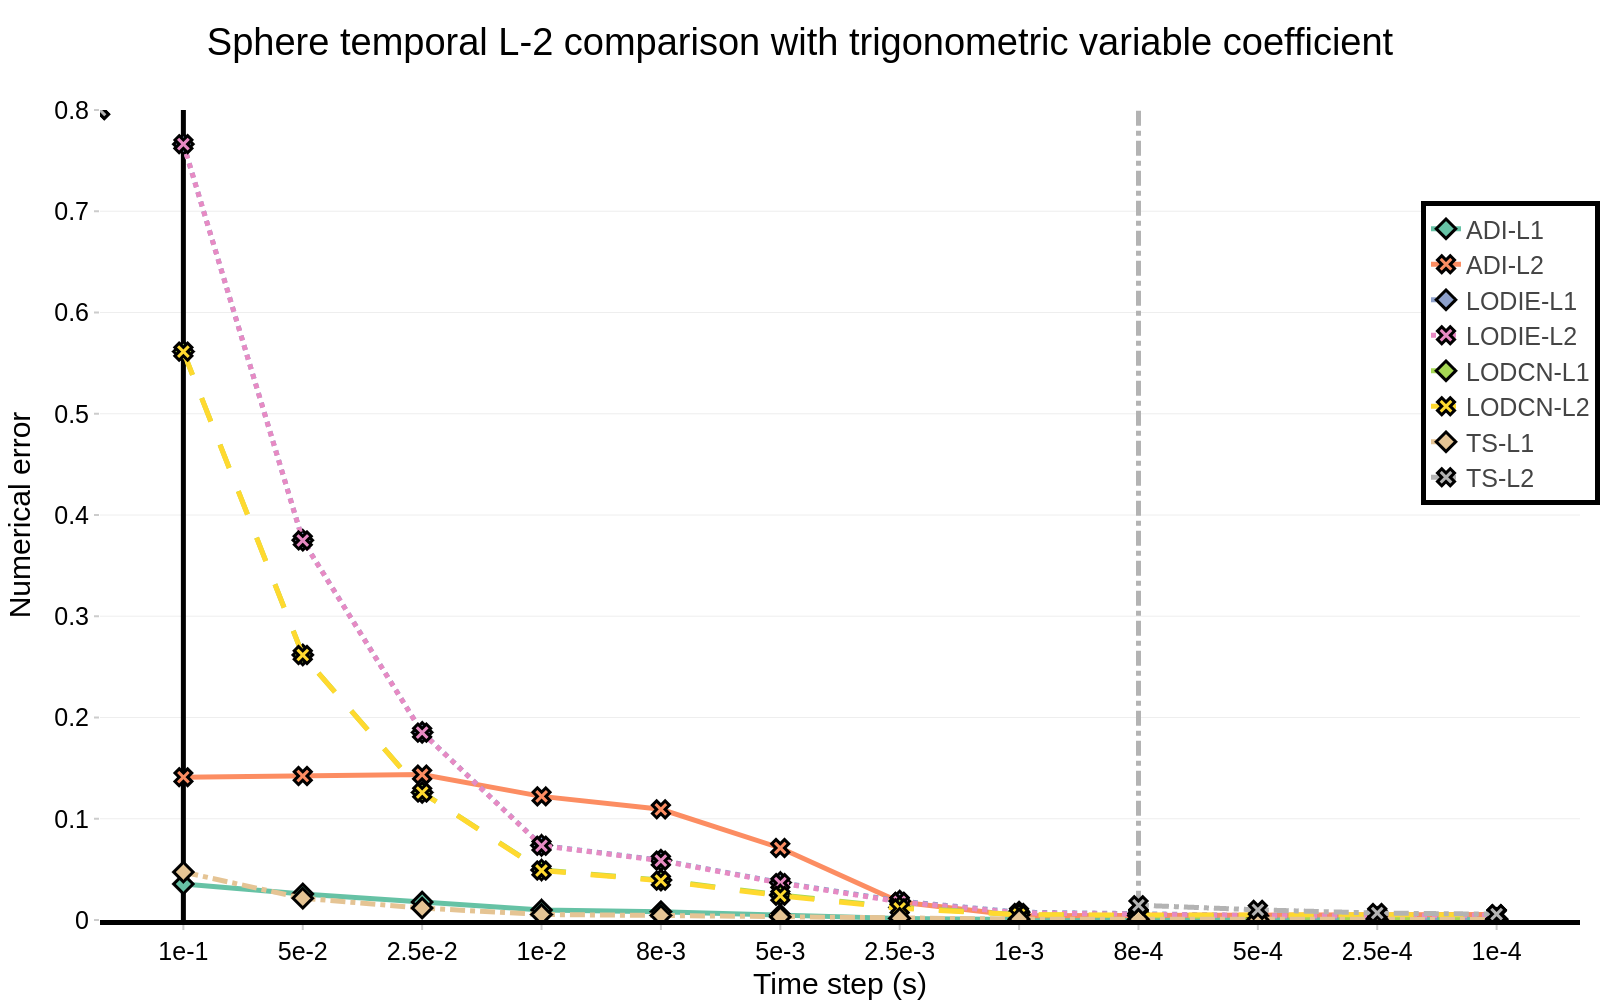
\includegraphics[width=13cm]{../figures/sphere_l2_2.png}
	\captionof{figure}{Temporal $L_{2}$ error for sphere interface with trigonometric type variable coefficient.}
	\label{fig:sphere_temporal_l2_type_2}
\end{figure}

\begin{figure}[!tb] 
	\centering
	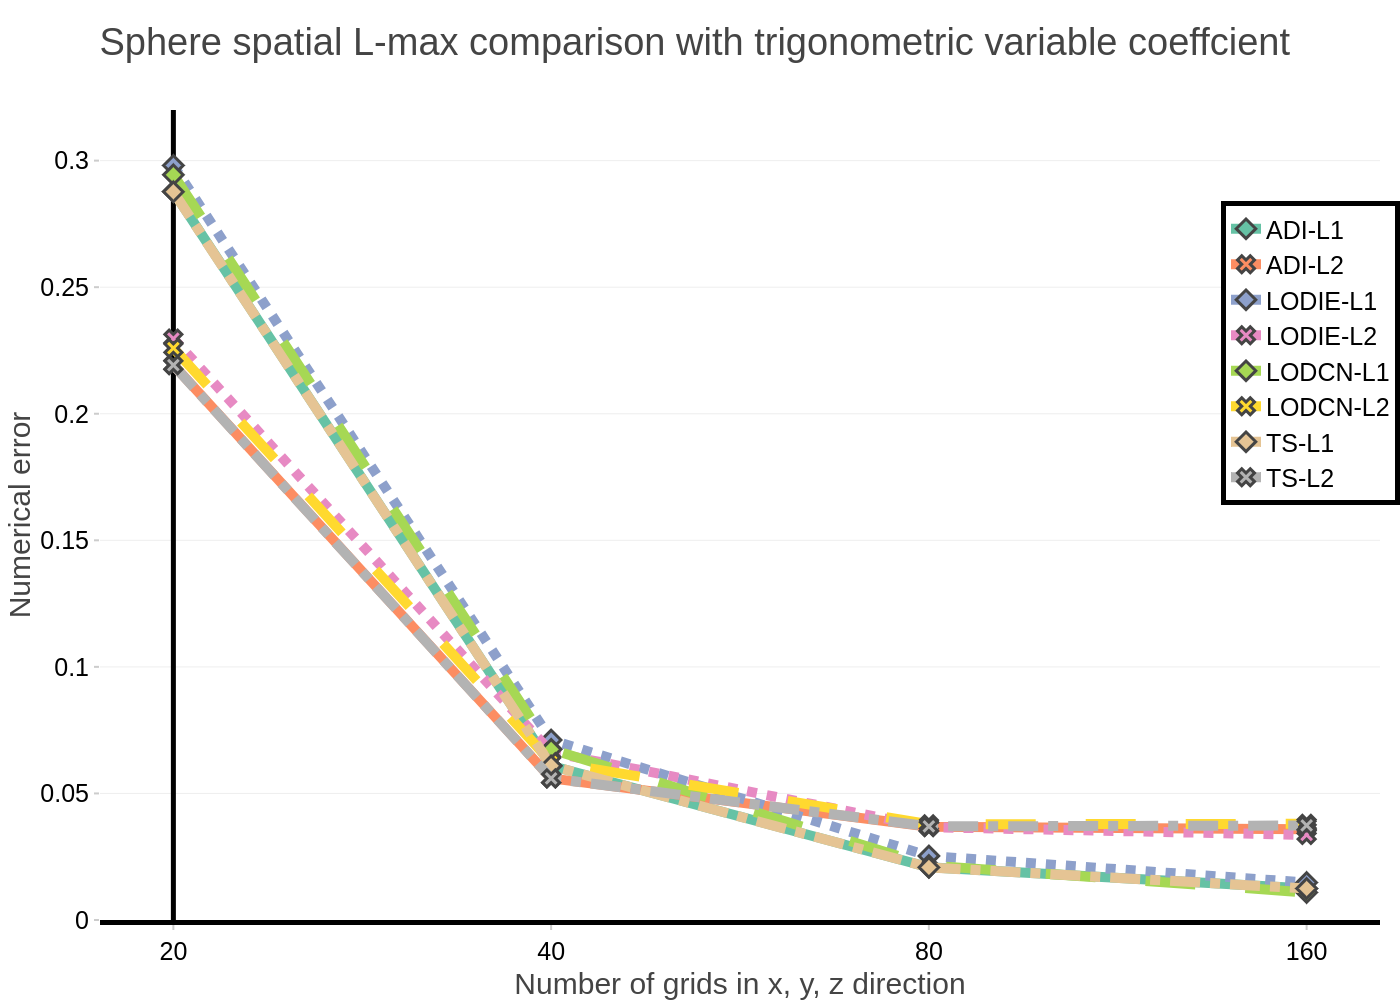
\includegraphics[width=13cm]{../figures/spatial_sphere_lmax_2.png}
	\captionof{figure}{Spatial $L_{\infty}$ error for sphere interface with trigonometric type variable coefficient.}
	\label{fig:sphere_spatial_lmax_type_2}
\end{figure}

\begin{figure}[!tb] 
	\centering
	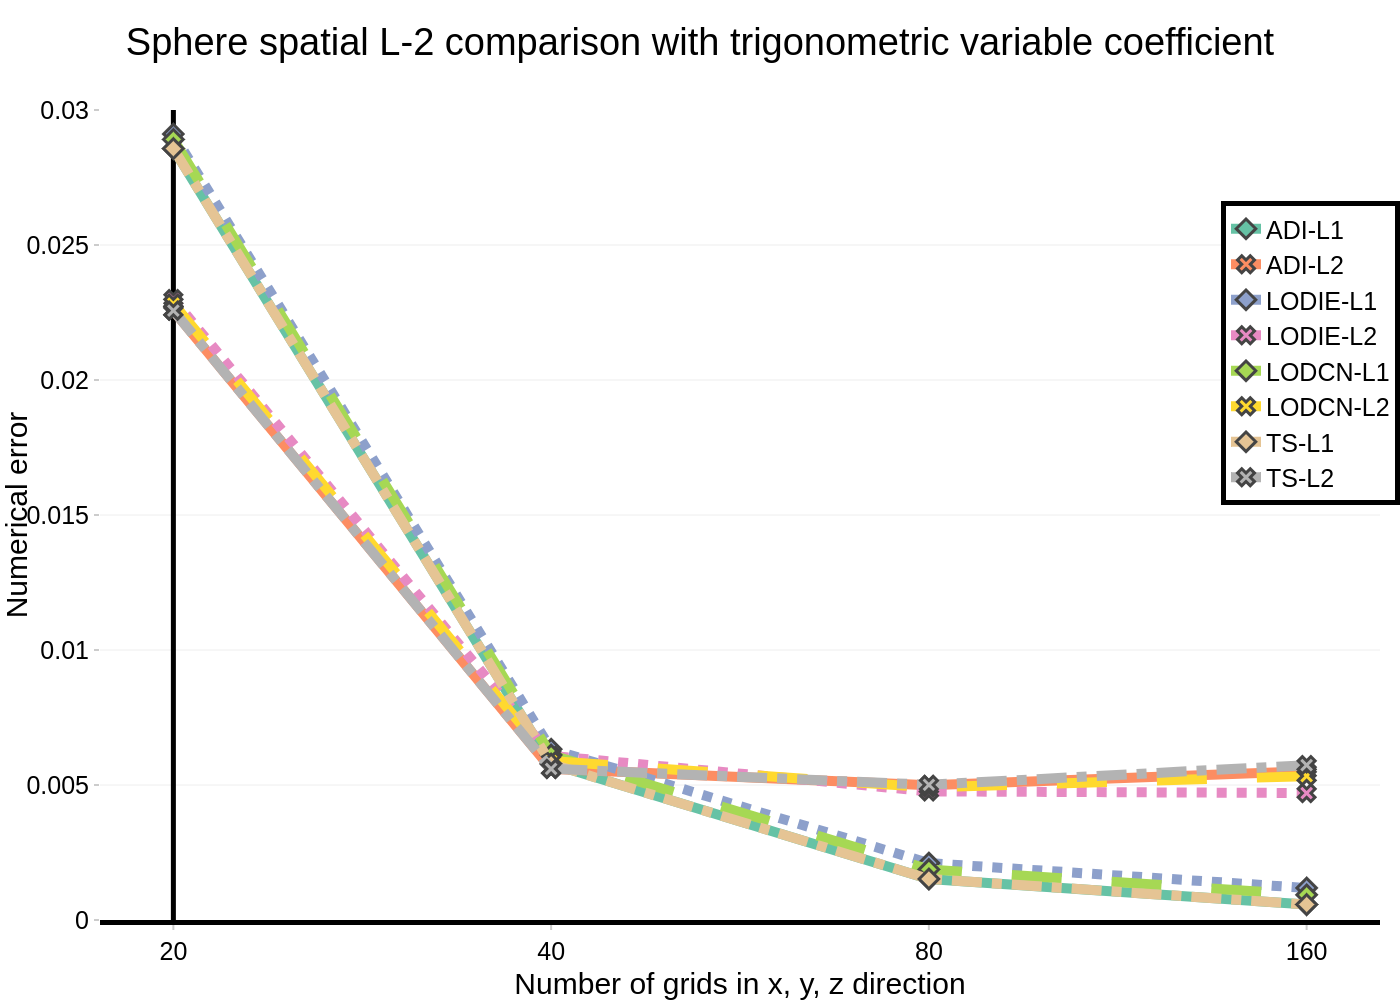
\includegraphics[width=13cm]{../figures/spatial_sphere_l2_2.png}
	\captionof{figure}{Spatial $L_{2}$ error for sphere interface with trigonometric type variable coefficient.}
	\label{fig:sphere_spatial_l2_type_2}
\end{figure}

For trigonometric type of variable coefficient, the efficiency is still the same that TS the most expensive one and LODIE the cheapest one shown in Figure \ref{fig:sphere_efficiency_2}. For temporal numerical error in Figure \ref{fig:sphere_temporal_lmax_type_2} and \ref{fig:sphere_temporal_l2_type_2}, TS-L2 is the only unstable one, unlike rational variable coefficients, it start convergence at $\Delta{t}=8e-4$ instead of $\Delta{t}=1e-3$. Meanwhile, none of the eight method can perform first order of convergence rate with respect to time. For spatial numerical error in Figure \ref{fig:sphere_spatial_lmax_type_1} and \ref{fig:sphere_spatial_l2_type_1}, time step is still fixed at $\Delta{t}=1e-4$ and different sizes of mesh grid are adopted, from 20 to 40, all algorithms converge with a rate 2, afterwards, none of them keep the convergence rate. Especially for $L_2$ error, methods with MIB-L2 scheme almost only keep the same error, while methods with MIB-L1 scheme still converge at a slow rate. 
%----------------------------------------------------------------------%
%                                                                      %
%                               Example 9                              %
%                                                                      %
%----------------------------------------------------------------------%

{\flushleft \bf Example 9.} The last example for the simple sphere interface (\ref{sphere}) with analytical solution (\ref{analytical_eqn_1}) and a computational domain $[-3.99,3.99]\times[-1.99,1.99]\times[-1.99,1.99]$ is tested in this example. The variable coefficient pair is referred to the Gaussian type (\ref{beta_3}).
%---------------------------- sphere type 3 ---------------------------------------
%
\begin{figure}[!tb] 
	\centering
	\includegraphics[width=13cm]{../figures/sphere_efficiency_3.png}
	\captionof{figure}{Sphere efficiency comparison with Gaussian type variable coefficient.}
	\label{fig:sphere_efficiency_3}
\end{figure}

\begin{figure}[!tb] 
	\centering
	\includegraphics[width=13cm]{../figures/sphere_lmax_3.png}
	\captionof{figure}{Temporal $L_{\infty}$ error for sphere interface with Gaussian type variable coefficient.}
	\label{fig:sphere_temporal_lmax_type_3}
\end{figure}

\begin{figure}[!tb] 
	\centering
	\includegraphics[width=13cm]{../figures/sphere_l2_3.png}
	\captionof{figure}{Temporal $L_{2}$ error for sphere interface with Gaussian type variable coefficient.}
	\label{fig:sphere_temporal_l2_type_3}
\end{figure}

\begin{figure}[!tb] 
	\centering
	\includegraphics[width=13cm]{../figures/spatial_sphere_lmax_3.png}
	\captionof{figure}{Spatial $L_{\infty}$ error for sphere interface with Gaussian type variable coefficient.}
	\label{fig:sphere_spatial_lmax_type_3}
\end{figure}

\begin{figure}[!tb] 
	\centering
	\includegraphics[width=13cm]{../figures/spatial_sphere_l2_3.png}
	\captionof{figure}{Spatial $L_{2}$ error for sphere interface with Gaussian type variable coefficient.}
	\label{fig:sphere_spatial_l2_type_3}
\end{figure}
%

The last type of variable diffusion coefficient for sphere is Gaussian function. In terms of efficiency in Figure \ref{fig:sphere_efficiency_3}, TS methods are still the most expensive methods. The temporal numerical errors are shown in Figure \ref{fig:sphere_temporal_lmax_type_3} and \ref{fig:sphere_temporal_l2_type_3}, The two LOD methods, LODIE and LODCN have a better convergence rate at the begining, since the error obtained from the two methods are relatively large than other methods. ADI method is the most accurate method, the error converge to a smaller range and bounded by the spatial size. For spatial numerical error in Figure \ref{fig:sphere_spatial_lmax_type_3} and \ref{fig:sphere_spatial_l2_type_3}, from 40 to 160, both $L_{\infty}$ and $L_2$ perform the theoritical rate of convergence equal to 2 in space and take minor improvements after the 40.
%----------------------------------------------------------------------%
%                                                                      %
%                               Example 10                             %
%                                                                      %
%----------------------------------------------------------------------%

{\flushleft \bf Example 10.} Besides the simple surface like sphere, a more complicated interface is taken into consideration as tanglecube we used in (\ref{tanglecube}) in a computational domain of dimension $[-3.99,3.99]\times[-3.99,3.99]\times[-4.99,4.99]$. The analytical solution is constructed in the same form of (\ref{analytical_eqn_2}) with $a=2$ with rational type of variable coefficient (\ref{beta_1}). 
%---------------------------- tanglecube type 1 ---------------------------------------
%
\begin{figure}[!tb] 
	\centering
	\includegraphics[width=13cm]{../figures/tanglecube_efficiency_1.png}
	\captionof{figure}{Tanglecube efficiency comparison with rational type variable coefficient.}
	\label{fig:tanglecube_efficiency_1}
\end{figure}

\begin{figure}[!tb] 
	\centering
	\includegraphics[width=13cm]{../figures/tanglecube_lmax_1.png}
	\captionof{figure}{Temporal $L_{\infty}$ error for tanglecube interface with rational type variable coefficient.}
	\label{fig:tanglecube_temporal_lmax_type_1}
\end{figure}

\begin{figure}[!tb] 
	\centering
	\includegraphics[width=13cm]{../figures/tanglecube_l2_1.png}
	\captionof{figure}{Temporal $L_{2}$ error for tanglecube interface with rational type variable coefficient.}
	\label{fig:tanglecube_temporal_l2_type_1}
\end{figure}

\begin{figure}[!tb] 
	\centering
	\includegraphics[width=13cm]{../figures/spatial_tanglecube_lmax_1.png}
	\captionof{figure}{Spatial $L_{\infty}$ error for tanglecube interface with rational type variable coefficient.}
	\label{fig:tanglecube_spatial_lmax_type_1}
\end{figure}

\begin{figure}[!tb] 
	\centering
	\includegraphics[width=13cm]{../figures/spatial_tanglecube_l2_1.png}
	\captionof{figure}{Spatial $L_{2}$ error for tanglecube interface with rational type variable coefficient.}
	\label{fig:tanglecube_spatial_l2_type_1}
\end{figure}
%

Consistent with the conclusion for simple surface, the two Trapezoidal splitting methods are the most inefficient one and the two LODIE methods are the most efficient one shown in Figure \ref{fig:tanglecube_efficiency_1}. In Figure \ref{fig:tanglecube_temporal_lmax_type_1}, ADI-L2 has the largest $L_{\infty}$ numerical error for this complicated interface, while it is the same as simple interface, the largest $L_2$ numerical error is still obtained from the two LODIE methods, in the meantime, TS-L2 remained the only conditionally stable methods. From Figure \ref{fig:tanglecube_spatial_lmax_type_1} and \ref{fig:tanglecube_spatial_l2_type_1}, it's hard to figure out the line segment with corresponding methods based on spatial numerical error comparison. The numerical results shows that all methods with MIB-L1 scheme perform a similar numerical error for both $L_{\infty}$ and $L_2$ which is significantly smaller than the numerical error generated by methods with MIB-L2 scheme. We have seen some comparable performance for sphere interface as well which indicates that MIB-L1 scheme converge better than MIB-L2 scheme.
%----------------------------------------------------------------------%
%                                                                      %
%                               Example 11                             %
%                                                                      %
%----------------------------------------------------------------------%

{\flushleft \bf Example 11.} Considering the same surface and analytical solution as previous example but replace the variable coefficient as a  type (\ref{beta_2}).

%---------------------------- tanglecube type 2 ---------------------------------------
\begin{figure}[!tb] 
	\centering
	\includegraphics[width=13cm]{../figures/tanglecube_efficiency_2.png}
	\captionof{figure}{Tanglecube efficiency comparison with trigonometric type variable coefficient.}
	\label{fig:tanglecube_efficiency_2}
\end{figure}

\begin{figure}[!tb] 
	\centering
	\includegraphics[width=13cm]{../figures/tanglecube_lmax_2.png}
	\captionof{figure}{Temporal $L_{\infty}$ error for tanglecube interface with trigonometric type variable coefficient.}
	\label{fig:tanglecube_temporal_lmax_type_2}
\end{figure}

\begin{figure}[!tb] 
	\centering
	\includegraphics[width=13cm]{../figures/tanglecube_l2_2.png}
	\captionof{figure}{Temporal $L_{2}$ error for tanglecube interface with trigonometric type variable coefficient.}
	\label{fig:tanglecube_temporal_l2_type_2}
\end{figure}

\begin{figure}[!tb] 
	\centering
	\includegraphics[width=13cm]{../figures/spatial_tanglecube_lmax_2.png}
	\captionof{figure}{Spatial $L_{\infty}$ error for tanglecube interface with trigonometric type variable coefficient.}
	\label{fig:tanglecube_spatial_lmax_type_2}
\end{figure}

\begin{figure}[!tb] 
	\centering
	\includegraphics[width=13cm]{../figures/spatial_tanglecube_l2_2.png}
	\captionof{figure}{Spatial $L_{2}$ error for tanglecube interface with trigonometric type variable coefficient.}
	\label{fig:tanglecube_spatial_l2_type_2}
\end{figure}
%

The efficiency comparison is illustrated in Figure \ref{fig:tanglecube_efficiency_2}. With regard to temporal numerical error in Figure \ref{fig:tanglecube_temporal_lmax_type_2} and \ref{fig:tanglecube_temporal_l2_type_2},, the same effect has been noticed for this complicated interface with trigonometric type of variable coefficients, ADI-L2 delivers the most inaccurate numerical results, which implies that the complexity of surface has a larger impact on $L_{\infty}$ than $L_2$. As far as spatial comparison for the eight methods in Figure \ref{fig:tanglecube_spatial_lmax_type_2} and \ref{fig:tanglecube_spatial_l2_type_2}, all methods with MIB-L1 schemes performs better than methods with MIB-L2 schemes, and the methods with MIB-L2 scheme stop converge after mesh size of 40.  

%----------------------------------------------------------------------%
%                                                                      %
%                               Example 12                             %
%                                                                      %
%----------------------------------------------------------------------%

{\flushleft \bf Example 12.} The last example we considered is still tanglecube surface with analytical solution (\ref{analytical_eqn_2}), Gaussian function is studied as (\ref{beta_3}).

In this example, efficiency can be interpreted from Figure \ref{fig:tanglecube_efficiency_3}. In Figure \ref{fig:tanglecube_temporal_lmax_type_3} and \ref{fig:tanglecube_temporal_l2_type_3}, only TS-L2 failed to converge when time step is relatively large, and all methods start converging after time step $\Delta{t}=5e-3$. Same with sphere interface, the ADI method performs less numerical error than other eventually. For Figure \ref{fig:tanglecube_spatial_lmax_type_3} and \ref{fig:tanglecube_spatial_l2_type_3}, this example keeps both characteristics of maintained by complicated interface and Gaussian type of variable coefficient. MIB-L1 scheme keep performs better than MIB-L2 scheme. Same as sphere, from mesh size 20 to 40, all methods with $L_{\infty}$ and $L_{2}$ converge with the theoritical rate, after 40, all just take small rate of convergence.
%---------------------------- tanglecube type 3 ---------------------------------------
\begin{figure}[!tb] 
	\centering
	\includegraphics[width=13cm]{../figures/tanglecube_efficiency_3.png}
	\captionof{figure}{Tanglecube efficiency comparison with Gaussian type variable coefficient.}
	\label{fig:tanglecube_efficiency_3}
\end{figure}

\begin{figure}[!tb] 
	\centering
	\includegraphics[width=13cm]{../figures/tanglecube_lmax_3.png}
	\captionof{figure}{Temporal $L_{\infty}$ error for tanglecube interface with Gaussian type variable coefficient.}
	\label{fig:tanglecube_temporal_lmax_type_3}
\end{figure}

\begin{figure}[!tb] 
	\centering
	\includegraphics[width=13cm]{../figures/tanglecube_l2_3.png}
	\captionof{figure}{Temporal $L_{2}$ error for tanglecube interface with Gaussian type variable coefficient.}
	\label{fig:tanglecube_temporal_l2_type_3}
\end{figure}

\begin{figure}[!tb] 
	\centering
	\includegraphics[width=13cm]{../figures/spatial_tanglecube_lmax_3.png}
	\captionof{figure}{Spatial $L_{\infty}$ error for tanglecube interface with Gaussian type variable coefficient.}
	\label{fig:tanglecube_spatial_lmax_type_3}
\end{figure}

\begin{figure}[!tb] 
	\centering
	\includegraphics[width=13cm]{../figures/spatial_tanglecube_l2_3.png}
	\captionof{figure}{Spatial $L_{2}$ error for tanglecube interface with Gaussian type variable coefficient.}
	\label{fig:tanglecube_spatial_l2_type_3}
\end{figure}

%
%----------------------------------------------------------------------%
%                                                                      %
%                             Chapter 5                                %
%                                                                      %
%----------------------------------------------------------------------%

\chapter{CONCLUSIONS}

\label{chap: conclusions}
In this work, we propose a novel matched ADI method for solving 3D parabolic interface problems with discontinuous diffusion coefficient and complex interfaces. The newly developed scheme inherits the merits of its ancestor for solving 2D interface problems, while possesses unique features, such as the non-orthogonal local coordinate system for decoupling the jump conditions, two-side estimation of tangential derivative at the interface point, and the capability of handling arbitrary many interface points on one grid line, for solving more challenging 3D problems. Moreover, a new Douglas-Rachford ADI scheme is designed, which minimizes the perturbation terms, in compared with the implicit Euler scheme, and is of first order in time. 

The proposed method is found to converge and maintains stability for various complex-shaped interfaces and time-and-space dependent jump conditions in the numerical experiments. Being highly accurate and efficient, this new ADI method provides a very promising numerical algorithm for solving 3D parabolic PDEs. In terms of accuracy, the matched ADI method yields a spatially second order of accuracy for all tested interface problems. Due to strong stability, a large time increment can be used in the ADI method for an efficient time integration. Moreover, in each time step, the ADI method provides an exact or non-iterative algebraic solver whose complexity scales linearly with respect to the spatial degree of freedom. Therefore, the matched ADI method is definitely one of the fastest implicit algorithms for solving 3D parabolic interface problems.

For variable coefficients, eight methods are proposed as ADI-L1, ADI-L2, LODIE-L1, LODIE-L2, LODCN-L1, LODCN-L2, TS-L1, TS-L2, which are named by a combination of temporal method and spatial method. Three different pairs of variable coefficient are deployed in numerical experiment with different types of analytical solutions. For efficiency, LODIE method are found to be the most efficient one, ADI method is almost same efficient as LODIE, LODCN method is much more expensive than the previous two methods and TS method is the most expensive one. Meanwhile, in spatial, MIB-L1 scheme is found slightly more efficient than MIBL2 method but with a little sacrifice of accuracy. For accuracy, it's interesting to say that there is not much difference between two spatial scheme MIB-L1 and MIB-L2 scheme. In terms of temporal methods, ADI method and TS method are much better than LODIE method and LODCN method. However, TS method is the only method that considered unstable with large time step, specially, TS method with MIB-L2 scheme, all other methods are stable with variable coefficient and various time step and grid size.

Overall, for solving parabolic interface problem, for the sake of its unconditional stability, high accuracy and extreme efficiency, matched ADI is the first choice to be considered regardless of constant diffusion coefficient or variable diffusion coefficient.


%----------------------------------------------------------------------%
%                                                                      %
%                             Reference                                %
%                                                                      %
%----------------------------------------------------------------------%
\addcontentsline{toc}{chapter}{REFERENCES}
\renewcommand{\bibname}{REFERENCES}
\bibliographystyle{acm}
\bibliography{mybib}

\iffalse
\addcontentsline{toc}{chapter}{REFERENCES}
\bibliographystyle{plain}
\bibliography{thesis-template}
\begin{singlespace}
\bibliography{stability}
\bibliographystyle{abbrv}
\label{bib}
\end{singlespace}

\begin{description}
	\item AKAIKE, H. (1973). Information theory and an extension of the maximum likelihood principle. In \emph{Second International Symposium on Information Theory}. Edited by Petrov,  B. N. and Csaki, F., 267--281. Budapest: Akademiai Kiado.
	
	\item Bottou, L. (2012). Stochastic gradient descent tricks. In \emph{Neural Networks: Tricks of the
	Trade}. Edited by Montavon, G., Orr, G., and Muller, K.-R., 421--436. Berlin Heidelberg: Springer.
	
\end{description}
\newpage
\fi

%%%%%%%%%%%%%%%%%%APPENDIX%%%%%%%%%%%%%%%%%%%%%%
%\addcontentsline{toc}{chapter}{APPENDIX}
%\appendix
%$\;$
%\vspace{1.5cm}
%\begin{center}
%	\textbf{{\normalsize APPENDIX}}
%\end{center}
%\vspace{0.3cm}
%In this appendix, .....


\end{body}
\end{document}
